% This is the Reed College LaTeX thesis template. Most of the work
% for the document class was done by Sam Noble (SN), as well as this
% template. Later comments etc. by Ben Salzberg (BTS). Additional
% restructuring and APA support by Jess Youngberg (JY).
% Your comments and suggestions are more than welcome; please email
% them to cus@reed.edu
%
% See http://web.reed.edu/cis/help/latex.html for help. There are a
% great bunch of help pages there, with notes on
% getting started, bibtex, etc. Go there and read it if you're not
% already familiar with LaTeX.
%
% Any line that starts with a percent symbol is a comment.
% They won't show up in the document, and are useful for notes
% to yourself and explaining commands.
% Commenting also removes a line from the document;
% very handy for troubleshooting problems. -BTS

% As far as I know, this follows the requirements laid out in
% the 2002-2003 Senior Handbook. Ask a librarian to check the
% document before binding. -SN

%%
%% Preamble
%%
% \documentclass{<something>} must begin each LaTeX document
\documentclass[12pt,a4paper,twoside]{ugathesis}
% Packages are extensions to the basic LaTeX functions. Whatever you
% want to typeset, there is probably a package out there for it.
% Chemistry (chemtex), screenplays, you name it.
% Check out CTAN to see: http://www.ctan.org/
%%
\usepackage{graphicx,latexsym}
\usepackage[french]{babel}
\usepackage{amsmath}
\usepackage{amssymb,amsthm}
\usepackage[dvipsnames]{xcolor} % tk: for more color
\usepackage{xcolor}
\usepackage{eso-pic}
\usepackage{longtable,booktabs,setspace}
\usepackage{chemarr} %% Useful for one reaction arrow, useless if you're not a chem major
\usepackage[hyphens]{url}
\usepackage{pdfpages}
\usepackage{tikz}
\usetikzlibrary{calc}
% Added by CII
\usepackage{hyperref}
\usepackage{lmodern}
\usepackage{float}
\floatplacement{figure}{H}
% End of CII addition
\usepackage{rotating}
\usepackage{upgreek} % tk : pour pouvoir utiliser le symbole µ droit (pas en itallic)
\usepackage{pdfpages} % tk : pour pouvoir insérer des fichiers pdf dans le corp de texte
\usepackage{lscape} % tk : pour pouvoir insérer des images au format paysage
\newcommand{\blandscape}{\begin{landscape}}
\newcommand{\elandscape}{\end{landscape}}
\usepackage[utf8]{inputenc}


% Next line commented out by CII
%%% \usepackage{natbib}
% Comment out the natbib line above and uncomment the following two lines to use the new
% biblatex-chicago style, for Chicago A. Also make some changes at the end where the
% bibliography is included.
%\usepackage{biblatex-chicago}
%\bibliography{thesis}


% Added by CII (Thanks, Hadley!)
% Use ref for internal links
\renewcommand{\hyperref}[2][???]{\autoref{#1}}
\def\chapterautorefname{Chapter}
\def\sectionautorefname{Section}
\def\subsectionautorefname{Subsection}
% End of CII addition

% Added by CII
\usepackage{caption}
\captionsetup{width=5in}
% End of CII addition

% \usepackage{times} % other fonts are available like times, bookman, charter, palatino



%%% Mise en page des titres (TK)
\titleformat{\chapter}[display]
{\vfill}
{{%
   \normalfont\fontsize{48pt}{48pt}\sffamily\color{red}\MakeUppercase{\chaptername}
   \fontsize{48pt}{48pt}\selectfont\thechapter%
 }%
}
{5pt}
{\Huge\normalfont
 \parbox{\textwidth-\widthof{\LARGE\sffamily\MakeUppercase{\chaptername}}}%
}[\vfill\clearpage]
\titlespacing*{\chapter}{0pt}{0pt}{0pt}
%%%





% To pass between YAML and LaTeX the dollar signs are added by CII
\title{THÈSE}
\author{Thomas Karaouzene}
\lab{Génétique, Epigénétique et Thérapies de l'Infertilité (GETI) et
Techniques de l'Ingénierie Médicale et de la Complexité - Informatique,
Mathématiques et Applications de Grenoble (TIMC-IMAG)}
\date{29 novembre 2017}
\division{Mathematics and Natural Sciences}
\advisor{Pierre Ray}
%If you have two advisors for some reason, you can use the following
% Uncommented out by CII
\altadvisor{Nicolas Thierry-Mieg}
% End of CII addition
%\institution{}
%\degree{}

%%% Remember to use the correct department!
\department{Ingénierie de la Santé, de la Cognition et Environnement (EDISCE)}
% if you're writing a thesis in an interdisciplinary major,
% uncomment the line below and change the text as appropriate.
% check the Senior Handbook if unsure.
%\thedivisionof{The Established Interdisciplinary Committee for}
% if you want the approval page to say "Approved for the Committee",
% uncomment the next line
%\approvedforthe{Committee}

% Added by CII
%%% Copied from knitr
%% maxwidth is the original width if it's less than linewidth
%% otherwise use linewidth (to make sure the graphics do not exceed the margin)
\makeatletter
\def\maxwidth{ %
  \ifdim\Gin@nat@width>\linewidth
    \linewidth
  \else
    \Gin@nat@width
  \fi
}
\makeatother

\renewcommand{\contentsname}{Table of Contents}
% End of CII addition

\setlength{\parskip}{0pt}

% Added by CII
  %\setlength{\parskip}{\baselineskip}
  \usepackage[parfill]{parskip}

\providecommand{\tightlist}{%
  \setlength{\itemsep}{0pt}\setlength{\parskip}{0pt}}

\Acknowledgements{

}

\Dedication{

}

\Preface{

}

\Abstract{

}

	\usepackage{tikz}
% End of CII addition
%%
%% End Preamble
%%
%

\usepackage{amsthm}
\newtheorem{theorem}{Theorem}[chapter]
\newtheorem{lemma}{Lemma}[chapter]
\theoremstyle{definition}
\newtheorem{definition}{Definition}[chapter]
\newtheorem{corollary}{Corollary}[chapter]
\newtheorem{proposition}{Proposition}[chapter]
\theoremstyle{definition}
\newtheorem{example}{Example}[chapter]
\theoremstyle{definition}
\newtheorem{exercise}{Exercise}[chapter]
\theoremstyle{remark}
\newtheorem*{remark}{Remark}
\newtheorem*{solution}{Solution}
\begin{document}

% Everything below added by CII
  \maketitle

\frontmatter % this stuff will be roman-numbered
\pagestyle{empty} % this removes page numbers from the frontmatter



  \hypersetup{linkcolor=black}
  \setcounter{tocdepth}{3}
  \tableofcontents

  \listoftables

  \listoffigures
rm 


\mainmatter % here the regular arabic numbering starts
\pagestyle{fancyplain} % turns page numbering back on

\chapter{If you are creating a PDF you'll need to write your preliminary
content here
or}\label{if-you-are-creating-a-pdf-youll-need-to-write-your-preliminary-content-here-or}

\chapter*{Remerciements}\label{remerciements}
\addcontentsline{toc}{chapter}{Remerciements}

\chapter*{Résumé}\label{resume}
\addcontentsline{toc}{chapter}{Résumé}

\chapter{Introduction}\label{introInf}

\newpage  

\section{L'ovogenèse}\label{lovogenese}

Les bases de l'ovogénèse (avec un petit schéma) the egg completes the
first meiosis and starts the second meiosis just prior to ovulation.
Second meiosis is arrested in metaphase and only resumes in case of
fertilization {[}\protect\hyperlink{ref-Tosti2016}{1}{]}

résumé de l'inrto PATL2

L'activation ovocytaire est produite chez l'ensemble des animaux par la
fertilisation d'un spermatozoïde. Celle-ci entrainera une augmentation
de la concentration cytosolique en Ca\textsuperscript{2+}
{[}\protect\hyperlink{ref-Stricker}{2}{]}. Chez les mamifères, la fusion
spermatozoïde-ovocyte est le déclencheur de séries distinctes
d'oscillations du Ca\textsuperscript{2+} cytosolique nécessaires au
développement normal de l'embryon
{[}\protect\hyperlink{ref-Stricker}{2},
\protect\hyperlink{ref-Miyazaki1993}{3}{]}. Ces observations on
rapidement permis l'emergence de l'hypothèse d'un facteur spermatique
qui, lors de la fécondation, était relargé et générait ces oscillations
Ca\textsuperscript{2+} {[}\protect\hyperlink{ref-Stricker}{2},
\protect\hyperlink{ref-Swann1990}{4}{]}. Cette hypothèse étant supportée
par deux principales observations. Tout d'abord, le fait que la fusion
des cytoplasmes du spermatozoïdes et de l'ovocytes était le prélude de
ces oscillations Des expermimentations
{[}\protect\hyperlink{ref-Sun1992}{5},
\protect\hyperlink{ref-Lawrence1997}{6}{]}. Ensuite, le fait que
l'injection d'un spermatozoïde ou d'extrait soluble de spermatozoïdes
entrainait des oscillations Ca\textsuperscript{2+} similaires à celles
observées lors de la fécondation
{[}\protect\hyperlink{ref-Swann1990}{4},
\protect\hyperlink{ref-Wu1997}{7}--\protect\hyperlink{ref-Tang2000}{10}{]}.
C'est en 2002 que la protéine PLC zeta (\(\zeta\)) fut pour la première
fois reporté comme étant, chez la souris, responsable de ces
oscillations déclachant ensuite une cascade de réactions dont découle
éventuellement l'activation ovocytaire et le développement embryonnaire
{[}\protect\hyperlink{ref-Saunders2002}{11}{]} (\textbf{Figure :}
\ref{fig:oocytefertilisation}).

\begin{figure}

{\centering \includegraphics[scale=.72]{figure/oocyte_fertilization} 

}

\caption[La fécondation, liaison spermatozoïde-ovocyte et sortie de la méiose]{\textbf{\emph{La fécondation, liaison
spermatozoïde-ovocyte et sortie de la méiose} adapté d'après
{[}\protect\hyperlink{ref-Clift2013}{12}{]}} : Suite à la fusion
spermatozoïde-ovocyte, la protéine PLCZ induit la production de nositol
1,4,5-trisphosphate (Ins(1,4,5)P\(_3\)) qui se lie à son recepteur
causant ainsi le relargage de Ca\textsuperscript{2+} qui, entre autre,
fera sortir l'ovocyte de son stade de méiose pour rentrer en mitose}\label{fig:oocytefertilisation}
\end{figure}









\section{La spermatogenèse}\label{la-spermatogenese}

La spermatogenèse des mammifères est un processus long et complexe
contrôlé par plusieurs mécanismes étroitement liés
{[}\protect\hyperlink{ref-Gnessi1997}{13}--\protect\hyperlink{ref-KIERSZENBAUM1994}{15}{]}.
C'est au cours de celle-ci, qu'à partir de cellules germinales, seront
produits les spermatozoïdes matures. Ce processus est divisé en trois
phases principales : la phase de multiplication, la phase de division
(appelée la \protect\hyperlink{meiose}{méiose}) et la phase de
maturation. Chez les hommes, ces étapes se déroulent en continu dans la
paroi des tubes séminifères du testicule depuis la puberté jusqu'à la
mort et impliquent trois types de cellules germinales : les
spermatogonies, les spermatocytes et les spermatides. Le temps
nécessaire pour obtenir un spermatozoïde mature à partir de cellules
germinales est de 74 jours et la production quotidienne de
spermatozoïdes s'élève environ à 45 millions par testicule
{[}\protect\hyperlink{ref-Johnson1980}{16}{]}. Le cycle
spermatogénétique est défini comme la succession chronologique des
différents stades de différenciation d'une génération de cellules
germinales (depuis la spermatogonie jusqu'au spermatozoïde). Chacune des
étapes du cycle spermatogénétique a une durée fixe et constante selon
les espèces (\textbf{Table : }\ref{tab:spermatotime}).

\begin{longtable}[t]{ll}
\caption{\label{tab:spermatotime}Durée de vie moyenne des cellules germinales humaines}\\
\toprule
Cellules germinales & Durée de vie moyenne (jours)\\
\midrule
Spermatogonies Ap & 16-18\\
Spermatogonie B & 7.5-9\\
Spermatocytes primaires & 23\\
Spermatocytes secondaires & 1\\
Spermatides & 1\\
\bottomrule
\end{longtable}

\newpage

\subsection{Rappels sur le testicule}\label{rappels-sur-le-testicule}

Les testicules sont les organes sexuels masculins. Ils possèdent deux
fonctions principales plus ou moins exprimées selon les périodes de la
vie de l'individu : une fonction endocrine caractérisée par la synthèse
des hormones stéroïdes sexuelles masculines (la stéroïdogenèse) et une
fonction exocrine au cours de laquelle seront produits les gamètes
masculins. Chez un individu adulte en bonne santé, le testicule présente
une forme ovoïde ayant un volume moyen de 18 cm\textsuperscript{3}. Chez
l'homme, comme chez la plupart des mammifères terrestres, ils sont
localisés sous le pénis dans une poche de peau appelée scrotum et reliés
à l'abdomen par le cordon spermatique (\textbf{Figure :}
\ref{fig:testicule}). Cette externalisation des testicules permet leur
maintien à une température plus basse que celle du reste du corps,
nécessaire à la spermatogenèse.

L'intérieur du testicule contient des tubes séminifères enroulés ainsi
que du tissu entre les tubules appelé espace interstitiel. Les tubes
séminifères sont de longs tubes compactés sous forme de boucles et dont
les deux extrémités débouchent sur le \emph{rete testis} (\textbf{Figure
:} \ref{fig:testicule}). C'est le long des parois du tube séminifère que
se déroulera l'ensemble des étapes de la spermatogenèse.

\begin{figure}

{\centering 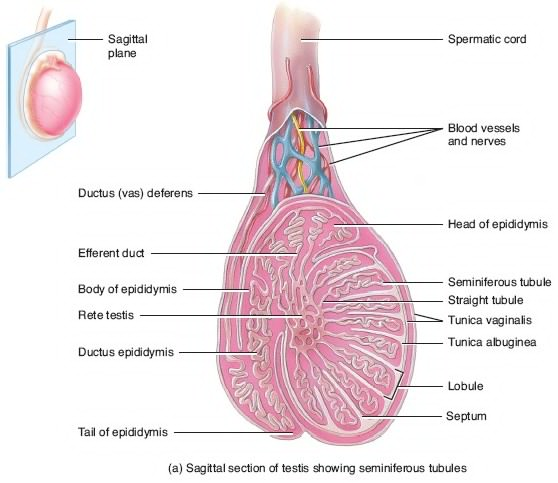
\includegraphics[scale=0.65]{figure/coupe_testicule2} 

}

\caption[Schéma anatomique du testicule humain]{\textbf{\emph{Schéma anatomique du testicule humain}.}}\label{fig:testicule}
\end{figure}



\newpage

\subsection{La phase de
multiplication}\label{la-phase-de-multiplication}

La phase de multiplication est la phase au cours de laquelle les
spermatogonies se divisent par mitoses pour aboutir au stade de
spermatocytes primaires. Les spermatogonies sont des cellules diploïdes
à l'origine de l'ensemble des autres cellules germinales humaines. Pour
cela, elles vont s'auto-renouveler par mitoses successives afin de
maintenir une production continue de spermatozoïdes tout au long de la
vie de l'individu. Ces cellules sont localisées dans le compartiment
basal des tubes séminifères. Les analyses histologiques ont permis de
distinguer trois types de spermatogonies en fonction de leur contenu en
hétérochromatine
{[}\protect\hyperlink{ref-Clermont1963}{17}--\protect\hyperlink{ref-Goossens2013}{19}{]}
: Les spermatogonies de type A dark (ou Ad), les spermatogonies de type
A pale (ou Ap) et les spermatogonies de type B.

Chez l'Homme, les spermatogonies Ad ont une activité mitotique au cours
de la spermatogenèse et servent de réserve. Elles vont au cours d'une
première mitose former une spermatogonie Ad et un spermatogonie Ap
(\textbf{Figure :} \ref{fig:spermatogenese}). Cette propriété permet à
la fois de se différencier en spermatocytes tout en constituant un
compartiment de réserve de spermatogonies Ad pour la régénération de la
population de cellules germinales au sein de l'épithélium séminifère.
L'entrée en division des spermatogonies Ap se fait par groupes
cellulaires tous les 16 jours. Les cellules d'une même génération
maintiennent entre elles des ponts cytoplasmiques jusqu'à la
\protect\hyperlink{spermiogenese}{spermiogenèse} ce qui permet la
synchronisation parfaite du développement gamétique de toutes les
cellules filles issues d'un groupe de spermatogonies Ap. Ce phénomène
est appelé onde spermatogénétique. Chaque spermatogonie Ap va former,
lorsqu'elle se divise par mitose, deux spermatogonies B qui elles-mêmes
se diviseront en deux spermatocytes primaires diploïdes (\textbf{Figure
:} \ref{fig:spermatogenese}).

\newpage

\begin{figure}

{\centering 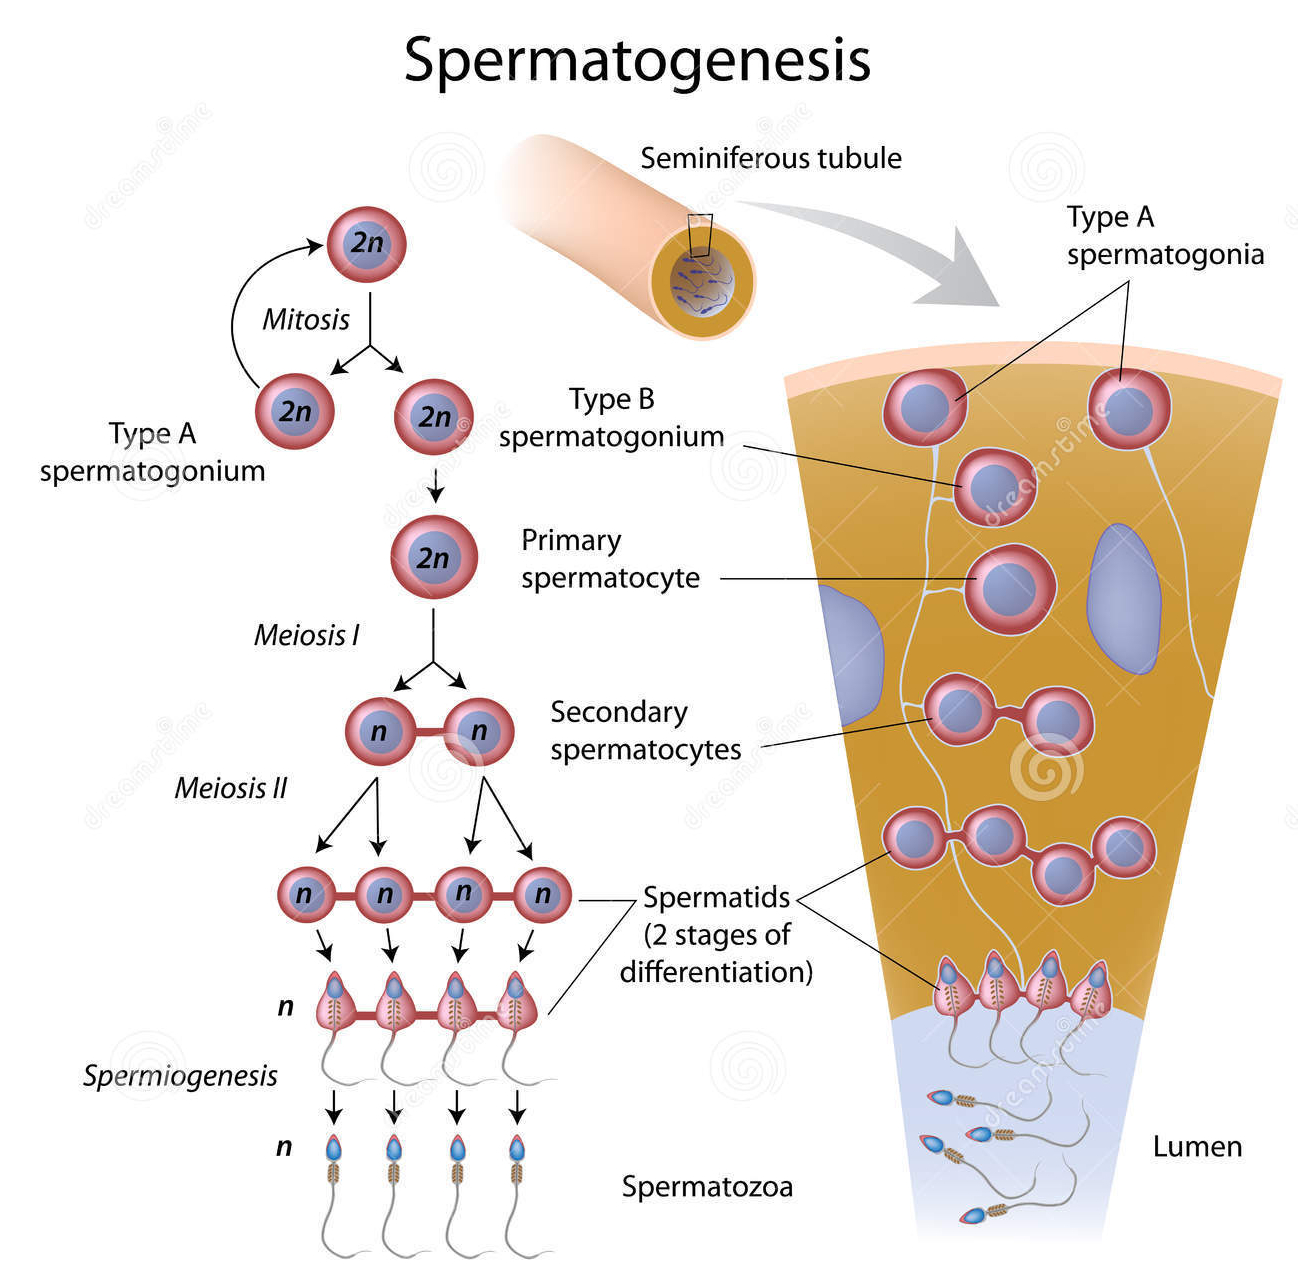
\includegraphics[scale=0.35]{figure/spermatogenese2} 

}

\caption[Les différentes phases de la spermatogenèse]{\textbf{\emph{Les différentes phases de la
spermatogenèse} d'après
\href{http://www.medizin-kompakt.de/spermatogenese}{medizin-kompakt}} :
L'évolution de la spermatogenèse est strictement coordonnée, tant dans
le sens transversal des tubules, que dans le sens longitudinal. Le sens
transversal correspond au sens unique de la différenciation germinale,
les cellules souches sont situées à la base du tube séminifère alors que
les spermatozoïdes aboutissent à la lumière. Dans le sens longitudinal
de ces tubules, on retrouve l'ensemble des cellules d'un même cycle
donnant ainsi l'onde spermatique.}\label{fig:spermatogenese}
\end{figure}












\newpage 

\hypertarget{meiose}{\subsection{La méiose}\label{meiose}}

La méiose, ou phase de maturation, est l'étape au cours de laquelle, à
partir de cellules diploïdes (les spermatogonies B) vont se former des
cellules haploïdes, les spermatocytes secondaires (spermatocytes II). Ce
résultat est le fruit de deux divisions successives (\textbf{Figure :
}\ref{fig:pictmeiose}) appelées respectivement méiose réductionnelle ou
méiose I (MI) et méiose équationnelle ou méiose II (MII). La MI va
séparer les chromosomes homologues, produisant deux cellules et
réduisant la ploïdie de diploïde à haploïde (d'où son nom
\emph{réductionnelle}). En plus de son rôle de division vu précédemment,
la méiose joue un rôle clef dans le brassage génétique (mélange des
gènes) et ce, grâce à deux mécanismes de brassage : le brassage
inter-chromosomique, lorsque les chromosomes sont séparés et le brassage
intra-chromosomique impliquant notamment des enjambements chromosomiques
(crossing-over) (\textbf{Figure : }\ref{fig:pictcrossingover}).

La méiose est initiée dès la fin de la phase de multiplication à partir
des spermatocytes primaires issus de la division des spermatogonies de
type B. Ces cellules nouvellement formées se situent dans le
compartiment basal du tube séminifère. C'est là qu'elles vont tout
d'abord subir une interphase (stade préleptotène) durant entre 2 et 4
jours. Au cours de cette phase a lieu la réplication de l'ADN. Cette
réplication se fait lorsque l'ADN est à l'état de chromatine, pendant la
phase S (pour synthèse) de l'interphase. À l'issue de cette phase,
chaque chromosome sera composé de deux chromatides reliées entre elles
par le centromère, le matériel génétique de chaque cellule ayant donc
été multiplié par deux. Par la suite, ces cellules vont subir deux
divisions méiotiques, chacune composée de quatre étapes distinctes
(\textbf{Figure : }\ref{fig:pictmeiose}) :

\begin{figure}

{\centering 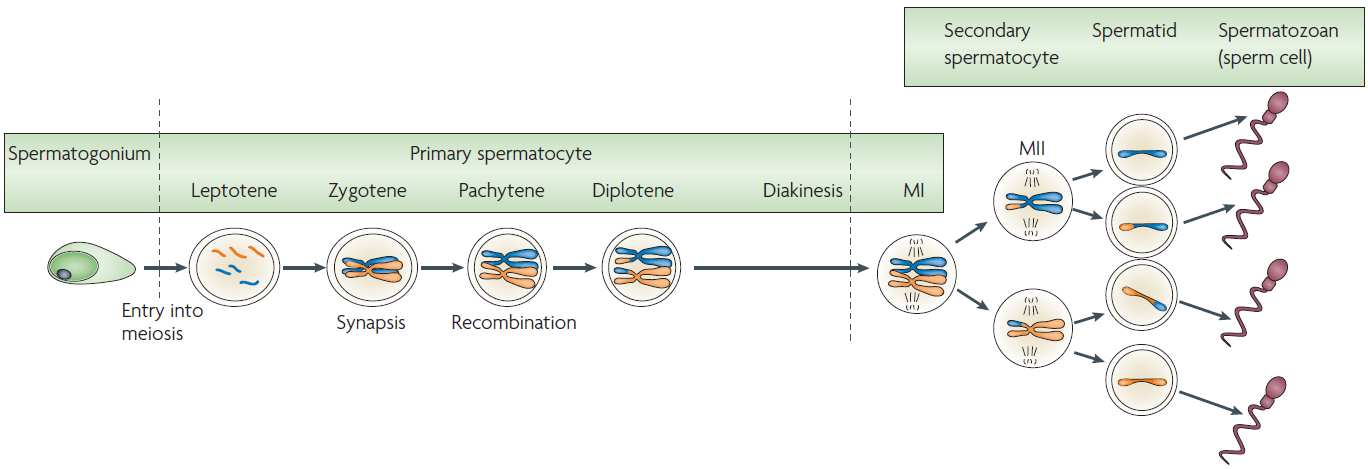
\includegraphics[scale=0.33]{figure/Meiosis_Stages} 

}

\caption[Les différentes étapes de la méiose gamétique masculine]{\textbf{\emph{Les différentes étapes de la méiose
gamétique masculine} d'après
{[}\protect\hyperlink{ref-Sasaki2008}{20}{]}} : Les spermatogonies B
servent de point d'initiation et se différentient en spermatocyte
primaire. Les cinq étapes de la prophase I sont suivies d'une première
division cellulaire, donnant deux cellules haploïdes au sein desquelles
les chromosomes sont composés de deux chromatides. Celles-ci seront
séparées au cours de la méiose II donnant ainsi quatre spermatides qui
après plusieurs étapes de maturation donneront les spermatozoïdes.}\label{fig:pictmeiose}
\end{figure}











\newpage

\begin{enumerate}
\def\labelenumi{\arabic{enumi}.}
\tightlist
\item
  \textbf{Méiose réductionnelle} : (\textbf{Figure : }\ref{fig:meiosei})

  \begin{enumerate}
  \def\labelenumii{\alph{enumii}.}
  \item
    \textbf{La prophase I} : cette longue étape dure 23 jours chez
    l'homme et peut être subdivisée en cinq phases successives :
    leptotène, zygotène, pachytène, diplotène et diacinèse.

    \begin{enumerate}
    \def\labelenumiii{\roman{enumiii}.}
    \tightlist
    \item
      \textbf{Leptotène} : condensation de la chromatine et formation
      des chromosomes.\\
    \item
      \textbf{Zygotène} : appariement des chromosomes homologues par
      paires appelés bivalents grâce à l'intermédiaire d'une structure
      multi-protéique : le complexe synaptonémal.\\
    \item
      \textbf{Pachytène} : ce stade dure 16 jours. Il est le plus long
      de la prophase I. C'est au cours de celui-ci, qu'a lieu l'échange
      de matériel génétique par le biais des crossing-over entre les
      chromatides non-sœurs appelées nodules de recombinaison
      (\textbf{Figure : }\ref{fig:pictcrossingover}).\\
    \item
      \textbf{Diplotène} : la dissociation du complexe synaptonémal va
      permettre aux chromosomes homologues d'initier leur séparation.
      Certains sites d'appariement étroits nommés chiasmas demeurent
      néanmoins liés permettant une séparation plus progressive des
      chromosomes et réduisant ainsi le risque d'aneuploïdies (nombre
      anormal de chromosomes)
      {[}\protect\hyperlink{ref-Handyside2012}{21}{]}.\\
    \item
      \textbf{Diacinèse} : cette étape marque la fin de la méiose I et
      fait office de transition avec la méiose II. Elle est caractérisée
      par une condensation maximale des chromosomes et la disparition de
      la membrane nucléaire et du nucléole. Le fuseau méiotique commence
      à s'assembler, les centromères des chromosomes homologues
      s'éloignent et les chiasmas glissent progressivement vers les
      télomères.\\
    \end{enumerate}
  \item
    \textbf{La métaphase I} : phase au cours de laquelle les chromosomes
    vont s'aligner à l'équateur de la cellule pour former la plaque
    équatoriale.
  \item
    \textbf{L'anaphase I} : les chromatides sœurs (ou les chromosomes
    homologues en fonction de la phase méiotique) vont se séparer et
    migrer aux pôles opposés de la cellule.\\
  \item
    \textbf{La télophase I} : qui est l'étape finale, les chromosomes se
    décondensent et l'enveloppe nucléaire se reforme autour des
    chromosomes. La cellule mère se sépare alors en deux cellules filles
    appelées spermatocytes secondaires.
  \end{enumerate}
\end{enumerate}

\newpage

\begin{enumerate}
\def\labelenumi{\arabic{enumi}.}
\setcounter{enumi}{1}
\tightlist
\item
  \textbf{Méiose équationnelle} : (\textbf{Figure : }\ref{fig:meioseii})
  la MII est similaire à une division mitotique et peut se décomposer en
  quatre parties distinctes :

  \begin{enumerate}
  \def\labelenumii{\alph{enumii}.}
  \tightlist
  \item
    \textbf{La prophase II} : contrairement à la prophase I, la prophase
    II est très courte. Les chromosomes alors formés de deux chromatides
    sœurs se dirigent vers la plaque équatoriale.\\
  \item
    \textbf{La métaphase II} : à ce stade, les chromosomes sont alignés
    le long de la plaque équatoriale au niveau de leur centromère.\\
  \item
    \textbf{L'anaphase II} : les centromères de chaque chromosome se
    séparent permettant aux chromatides sœurs de se diriger vers les
    pôles opposés des spermatocytes II.\\
  \item
    \textbf{La télophase II} : comme en télophase I, les cellules mères
    se séparent en deux cellules filles haploïdes appelées spermatides,
    contenant chacune n chromosomes.
  \end{enumerate}
\end{enumerate}

\begin{figure}

{\centering 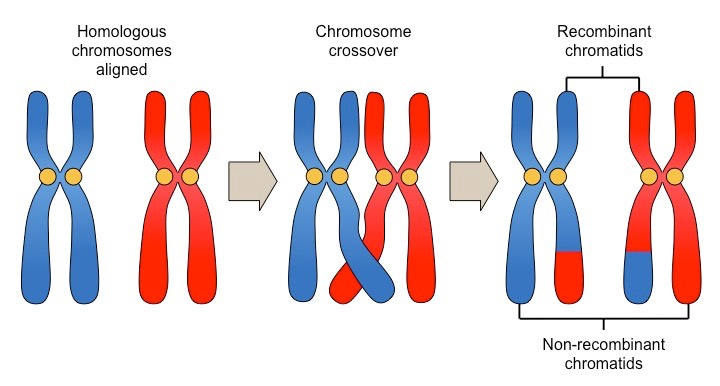
\includegraphics[scale=0.35]{figure/crossingover} 

}

\caption[Schéma simplifié d'un enjambement chromosomique (crossing-over)]{\textbf{\emph{Schéma simplifié d'un enjambement
chromosomique (crossing-over)}.}}\label{fig:pictcrossingover}
\end{figure}




\newpage 

\begin{figure}

{\centering 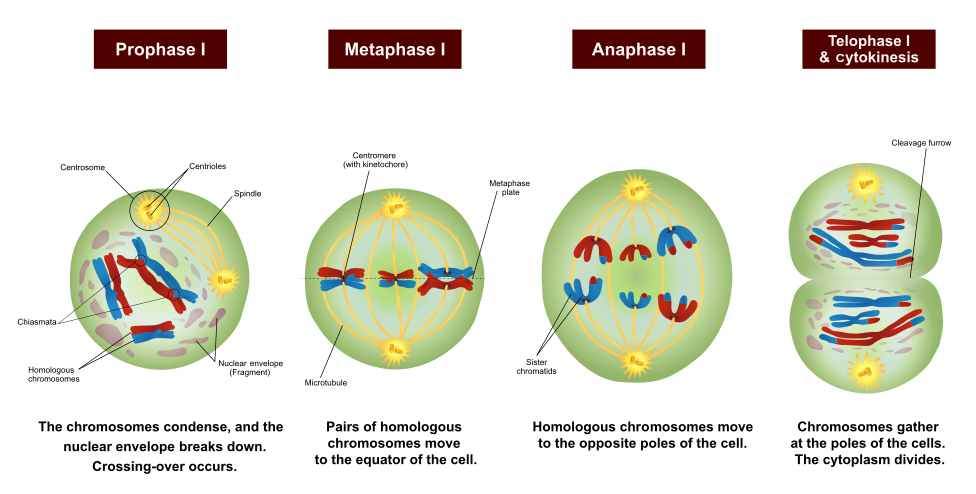
\includegraphics[scale=0.43]{figure/MeiosisI} 

}

\caption[Les différentes étapes de la première division méiotique masculine]{\textbf{\emph{Les différentes étapes de la première
division méiotique masculine} adapté d'après
{[}\protect\hyperlink{ref-Reece2014}{22}{]}}.}\label{fig:meiosei}
\end{figure}





\begin{figure}

{\centering 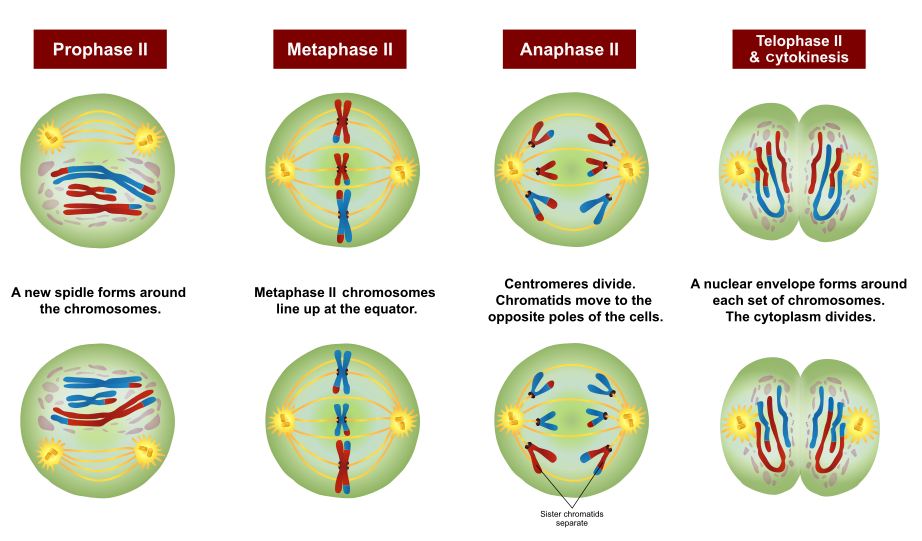
\includegraphics[scale=0.43]{figure/MeiosisII} 

}

\caption[Les différentes étapes de la deuxième division méiotique masculine]{\textbf{\emph{Les différentes étapes de la deuxième
division méiotique masculine} adapté d'après
{[}\protect\hyperlink{ref-Reece2014}{22}{]}}.}\label{fig:meioseii}
\end{figure}





\newpage

\hypertarget{spermiogenese}{\subsection{La
spermiogenèse}\label{spermiogenese}}

La spermiogenèse est la phase finale de la spermatogenèse. Elle dure
environ 23 jours chez l'humain et peut être subdivisée en sept étapes
(\textbf{Figure : }\ref{fig:spermiogenese}). La spermiogenèse définit la
cytodifférentiation des spermatides en spermatozoïdes. C'est au cours de
cette phase que les caractéristiques morphologiques et fonctionnelles du
spermatozoïde seront déterminées
{[}\protect\hyperlink{ref-YvesClermontRichardOko1993}{23}{]}. Elle est
caractérisée par trois évènements majeurs : la formation de l'acrosome,
la compaction de l'ADN nucléaire et la formation du flagelle. Le
développement de l'acrosome et la formation du flagelle commencent au
niveau des spermatides rondes
{[}\protect\hyperlink{ref-Escalier1991}{24}{]}. Pendant l'élongation de
la spermatide, le noyau se condense et devient hautement polarisé
{[}\protect\hyperlink{ref-Hamilton1987}{25}{]}. Les spermatides sont
situées dans le compartiment adluminal, à proximité de la lumière du
tube séminifère. Ce sont de petites cellules (8 à 10 \(\upmu\)m) que
l'on peut schématiquement diviser en trois classes :

\begin{enumerate}
\def\labelenumi{\arabic{enumi}.}
\item
  \textbf{Les spermatides rondes} (\textbf{Figure :
  }\ref{fig:spermiogenese} - \textbf{1} et \textbf{2}) :
  l'identification de ces cellules représente une difficulté technique.
  Elles ont cependant pu être décrites en détail par différentes
  techniques de coloration sous microscope optique
  {[}\protect\hyperlink{ref-Clermont1963}{17},
  \protect\hyperlink{ref-Papic}{26}--\protect\hyperlink{ref-WorldHealthOrganization1992}{29}{]}.
  Plusieurs études animales ont pu démontrer le potentiel des
  spermatides rondes à donner la vie à des individus sains et fertiles,
  {[}\protect\hyperlink{ref-Ogura1994}{30}--\protect\hyperlink{ref-Sasagawa}{32}{]},
  la même chose ayant été également observée plus récemment chez l'homme
  {[}\protect\hyperlink{ref-Tanaka2015}{33}{]} bien que le taux de
  fécondation et d'implantation soit extrêmement faible
  {[}\protect\hyperlink{ref-Asimakopoulos2003}{34}{]}. Ils possèdent un
  noyau rond avec une chromatine pâle et homogène. C'est à partir de ces
  étapes que démarre la biogenèse de l'acrosome avec la production par
  l'appareil de Golgi des vésicules pro-acrosomales (phase de Golgi).
  Les deux centrioles contenus dans le cytoplasme vont se déplacer au
  futur pôle caudal. Le centriole proximal est inactif alors que le
  centriole distal donne naissance à un ensemble de microtubules à
  l'origine de l'axonème du futur flagelle.
\item
  \textbf{Les spermatides en élongation} (\textbf{Figure :
  }\ref{fig:spermiogenese} - \textbf{3} et \textbf{4}) : à ce stade,
  l'acrosome va s'étendre le long du noyau lui donnant une forme plus
  allongée et la chromatine devient plus sombre. Un réseau de
  microtubules se forment autour du noyau créant ainsi la manchette qui
  participera également à l'allongement de la tête du spermatozoïde et
  permettra la migration des mitochondries vers la pièce intermédiaire
  du flagelle pour former le manchon de mitochondries
  {[}\protect\hyperlink{ref-Moreno2006}{35}{]}. Les spermatides en
  élongation peuvent aussi permettre la fécondation et d'initier des
  grossesses avec un meilleur taux de réussite que les spermatides
  rondes. De plus, ils engendreraient théoriquement moins de risques
  d'anomalies génétiques
  {[}\protect\hyperlink{ref-Asimakopoulos2003}{34}{]}.
\end{enumerate}

\newpage

\begin{enumerate}
\def\labelenumi{\arabic{enumi}.}
\setcounter{enumi}{2}
\tightlist
\item
  \textbf{Les spermatides en condensation} (\textbf{Figure :
  }\ref{fig:spermiogenese} - \textbf{5} et \textbf{7}) : c'est le stade
  final de la différenciation du spermatide en spermatozoïde. À ce stade
  le noyau est très allongé, avec une partie caudale globulaire et une
  partie antérieure saillante. La chromatine est sombre et condensée.
  L'axonème va continuer à s'allonger pour former le flagelle mature.
  Les différentes organelles inutiles pour la physiologique spermatique
  et l'excès de cytoplasme vont former la gouttelette cytoplasmique qui
  va se détacher et donner le corps résiduel qui va ensuite être
  phagocyté par les cellules de Sertoli
  {[}\protect\hyperlink{ref-Hermo2010}{36}{]}.
\end{enumerate}

Une fois ces étapes de différentiation finies, les spermatides sont
relâchées en tant que spermatozoïdes dans la lumière du tube séminifère.
Ce procédé est appelé spermiation.

\begin{figure}

{\centering 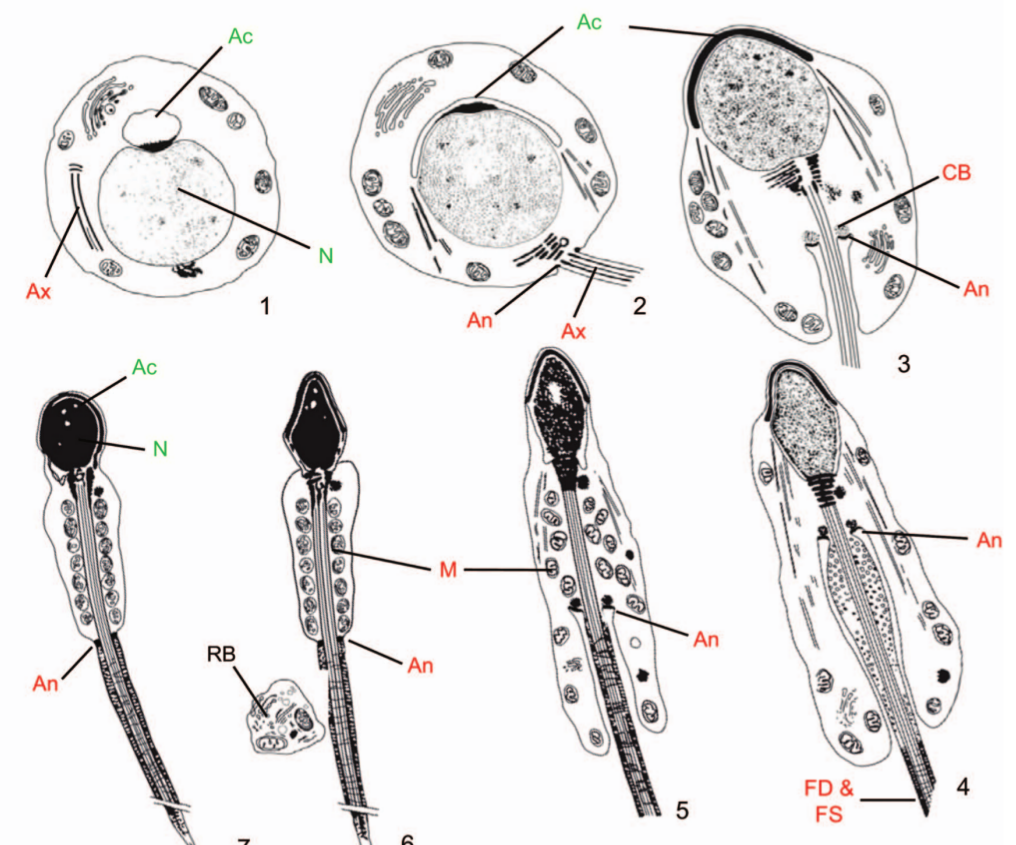
\includegraphics[scale=0.3]{figure/spermiogenese} 

}

\caption[Principales étapes et modifications structurales lors de la spermiogenèse]{\textbf{\emph{Principales étapes et modifications
structurales lors de la spermiogenèse} d'après
{[}\protect\hyperlink{ref-Toure2011}{37}{]}} : \textbf{1.} La spermatide
immature avec un gros noyau arrondi. La vésicule acrosomale est attachée
au noyau, l'ébauche du flagelle n'atteint pas le noyau. \textbf{2.} La
vésicule acrosomale a augmenté de taille et apparaît aplatie au niveau
du noyau. Le flagelle entre en contact avec le noyau. \textbf{3-7.}
Formation de l'acrosome, condensation du noyau et développement des
structures flagellaires. Ac = Acrosome, Ax = Axonème, CC = Corps
Chromatoïdes, CR = Corps Résiduel, FD = Fibres Denses, GF = Gaine
Fibreuse, M = Mitochondrie, Ma = Manchette.}\label{fig:spermiogenese}
\end{figure}













\newpage  

\section{Structure et fonction du
spermatozoïde}\label{structure-et-fonction-du-spermatozoide}

Le spermatozoïde est une cellule hautement différenciée dont la taille,
l'orientation et la symétrie sont déterminées. La morphologie générale
du spermatozoïde éjaculé est similaire à celle du spermatozoïde
testiculaire. Le spermatozoïde humain normal mature mesure environ 60
\(\upmu\)m de long et est essentiellement constitué de deux parties : la
tête et le flagelle (\textbf{Figure : }\ref{fig:spz}). En plus d'être
unique dans sa morphologie, le spermatozoïde l'est aussi dans sa
fonction puisque c'est la seule cellule produite de manière endogène et
dont l'action est exercée de manière exogène. La fécondation d'un
ovocyte par un spermatozoïde formera un zygote diploïde qui pourra se
développer ensuite en embryon dans l'utérus féminin.




\begin{figure}

{\centering 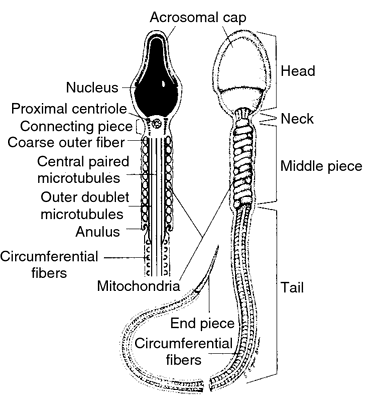
\includegraphics[scale=.75]{figure/sperm_anatomy} 

}

\caption[Anatomie simplifiée du spermatozoïde]{\textbf{\emph{Anatomie simplifiée du spermatozoïde} d'après
\href{http://medical-dictionary.thefreedictionary.com/Human+sperm}{medical-dictionary}}.}\label{fig:spz}
\end{figure}

\newpage

\subsection{La tête}\label{la-tete}

\begin{enumerate}
\def\labelenumi{\arabic{enumi}.}
\item
  \textbf{L'acrosome} : c'est une vésicule de sécrétion géante située
  dans la moitié supérieure de la tête du spermatozoïde. Elle se
  développe à partir de l'appareil de Golgi lors de la spermiogenèse. Au
  cours de sa formation, l'acrosome forme tout d'abord un granule
  sphérique qui se colle sur la partie apicale du noyau. En
  s'aplatissant contre celui-ci, l'acrosome va prendre une forme
  hémisphérique recouvrant la membrane nucléaire formant la coiffe
  céphalique. Le rôle de l'acrosome est fondamental dans le processus de
  fécondation puisqu'il permet d'excréter notamment l'acrosine, une
  enzyme de digestion permettant au spermatozoïde de traverser la zone
  pellucide qui entoure les ovocytes. Ce processus de relargage est
  appelé réaction acrosomale.
\item
  \textbf{L'acroplaxome} : l'acroplaxome est une structure cytosquelette
  composée de microfilaments d'actine (F- actine) et de kératine 5.
  Cette structure est positionnée en face de l'appareil de golgi et
  contre le noyau et sert de point d'attachement ainsi que de guide aux
  vésicules pro-acrosomales
  {[}\protect\hyperlink{ref-Kierszenbaum2004}{38}{]}. C'est une
  structure transitoire qui disparaît pour être remplacée par la thèque
  périnucléaire dans le spermatozoïde mature.
\item
  \textbf{Le noyau} : c'est une structure cellulaire présente dans la
  majorité des cellules eucaryotes. Il contient l'essentiel du matériel
  génétique. Le noyau du spermatozoïde est caractérisé par une
  compaction extrêmement importante de l'ADN. Dans les cellules
  somatiques l'ADN est enroulé par unité de 146 paires de bases autour
  d'un octamère d'histones dit de cœur (H2A, H2B, H3 et H4) afin
  d'organiser les trois milliards de paires de bases du génome humain
  dans un noyau de quelques microns (\textbf{Figure : }\ref{fig:noyau}).
  L'ADN des spermatides va subir une réorganisation chromatinienne plus
  importante au cours de la spermatogenèse afin d'augmenter sa
  compaction. Ainsi, les octamères d'histones présents dans les cellules
  somatiques sont remplacés par les protéines de transition (TPN1, TPN2)
  puis par les protamines (PRM1, PRM2), deux protéines riches en
  arginine et en cystéine (\textbf{Figure : }\ref{fig:noyau}).
  L'intégrité des deux protéines composant ce dimère est nécessaire pour
  la procréation {[}\protect\hyperlink{ref-Cho2001}{39}{]}. Cette
  compaction extrême permet de réduire la taille du noyau, mais aussi de
  protéger l'ADN d'agents de dégradation comme l'oxydation des bases.
  Parallèlement à cette condensation chromatinienne se produit un arrêt
  des processus de transcription cellulaire
  {[}\protect\hyperlink{ref-Kierszenbaum1978}{40}{]}. Le noyau du
  spermatozoïde est donc un noyau au repos, transcriptionnellement
  inactif {[}\protect\hyperlink{ref-Ward1994}{41}{]}.
\end{enumerate}

\newpage

\begin{figure}

{\centering 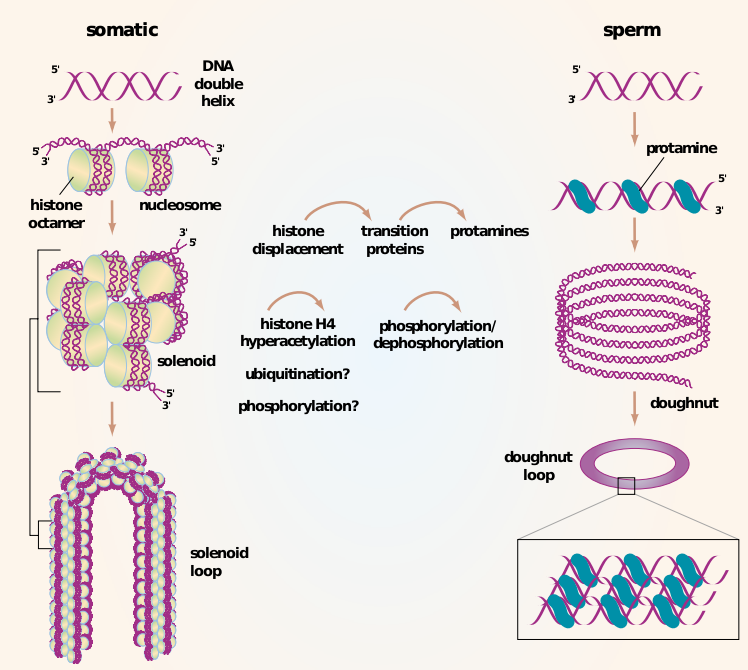
\includegraphics[scale=.55]{figure/noyau} 

}

\caption[Schéma de la compaction de l’ADN dans les cellules somatiques et dans les spermatozoïdes]{\textbf{\emph{Schéma de la compaction de l'ADN dans les
cellules somatiques et dans les spermatozoïdes} d'après
{[}\protect\hyperlink{ref-Braun2001}{42}{]}} : Dans les cellules
somatiques, l'ADN est enroulé sous forme de nucléosome. Les nucléosomes
vont s'agencer entre eux pour former un solénoïde qui sera attaché à la
matrice nucléaire par sa base. Dans le noyau spermatique les nucléosomes
sont remplacés par des protamines qui vont compacter l'ADN sous forme de
``\emph{doughnut}''. Le remplacement des histones est facilité par des
acétylations, des ubiquitinations et des phosphorylations.}\label{fig:noyau}
\end{figure}











\newpage

\subsection{Le flagelle}\label{le-flagelle}

Le flagelle représente la queue du spermatozoïde. Celui-ci permet, par
mouvements d'oscillation à haute vitesse, le déplacement du
spermatozoïde. Cette mobilité est générée par un cytosquelette interne
extrêmement conservé durant l'évolution appelé l'axonème. Celui-ci est
composé de neuf doublets de microtubules périphériques et de deux
doublets internes {[}\protect\hyperlink{ref-Inaba2003}{43}{]}
(\textbf{Figure : }\ref{fig:pictaxoneme}), on parle alors de structure
``9 + 2''. Les doublets externes sont reliés entre eux par des ponts de
nexine et au doublet central par des ponts radiaires. Les doublets
externes sont également reliés entre eux par les complexes protéiques
qui forment les dynéines externes et internes. Ce sont ces protéines qui
en exerçant une contraction alternée permettent le mouvement du
spermatozoïde.







\begin{figure}

{\centering 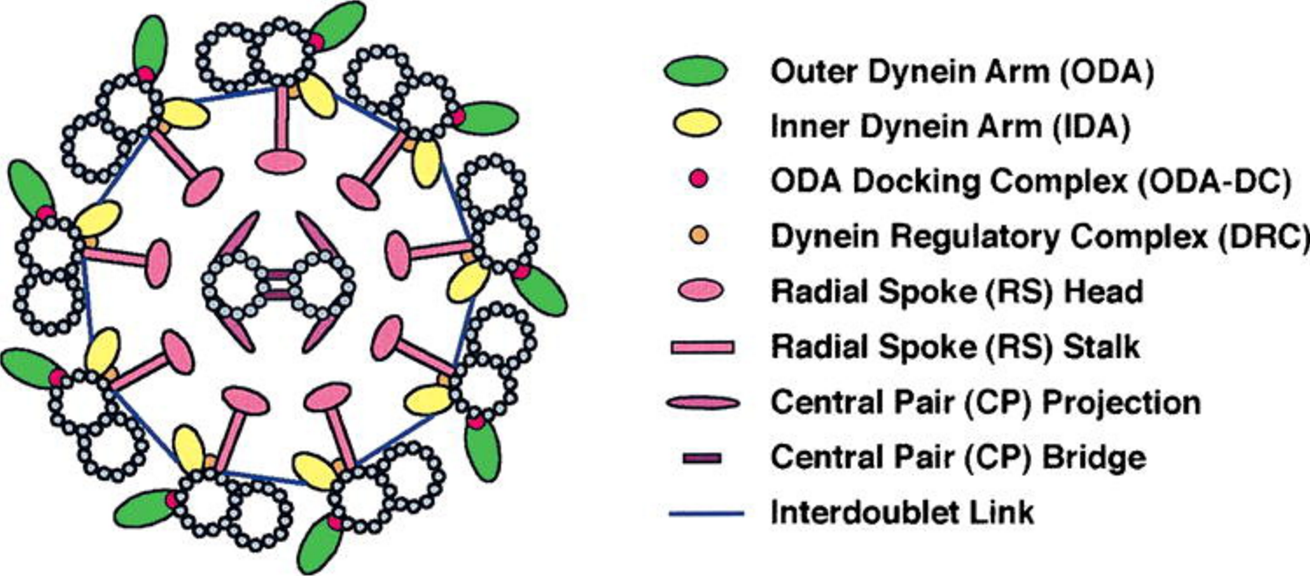
\includegraphics[scale=.3]{figure/axoneme} 

}

\caption[Structure simplifiée de l'axonème]{\textbf{\emph{Structure simplifiée de l'axonème}
d'après {[}\protect\hyperlink{ref-Inaba2003}{43}{]}} : L'axonème est
constitué de neuf doublets de microtubules périphériques reliés entre
eux par des liens de nexine et d'un doublet central relié aux doublets
périphériques par des ponts radiaires.}\label{fig:pictaxoneme}
\end{figure}

Le flagelle du spermatozoïde peut être divisé en trois parties
distinctes (\textbf{Figure : }\ref{fig:flagelle}) :

\begin{enumerate}
\def\labelenumi{\arabic{enumi}.}
\tightlist
\item
  \textbf{La pièce intermédiaire} : elle fait jonction avec la tête du
  spermatozoïde. Elle est composée de la gaine de mitochondrie qui
  fournira une partie de de l'énergie nécessaire au battement
  flagellaire (grâce à la phosphorylation oxydative qui produit de
  l'ATP). L'axonème qui se prolonge dans la pièce principale est un
  ensemble de neuf faisceaux de fibres denses.
\end{enumerate}

\newpage

\begin{enumerate}
\def\labelenumi{\arabic{enumi}.}
\setcounter{enumi}{1}
\tightlist
\item
  \textbf{La pièce principale} : ici, la gaine de mitochondrie a disparu
  ainsi que deux des faisceaux de fibres denses présents dans la pièce
  intermédiaire. On note cependant la présence d'une structure
  supplémentaire, la gaine fibreuse. Cette gaine entoure l'axonème et
  comporte deux épaississements diamétralement opposés, appelés colonnes
  longitudinales sur lesquelles s'insèrent les fibres denses 3 et 8.
  C'est le long de la gaine fibreuse qu'est produit la majorité de
  l'énergie nécessaire au glissement des microtubules
  {[}\protect\hyperlink{ref-Eddy2007}{44}{]}.\\
\item
  \textbf{La pièce terminale} : elle est située au niveau de l'extrémité
  distale du flagelle et ne contient que l'axonème
  {[}\protect\hyperlink{ref-Inaba2003}{43}{]}.
\end{enumerate}

\begin{figure}

{\centering 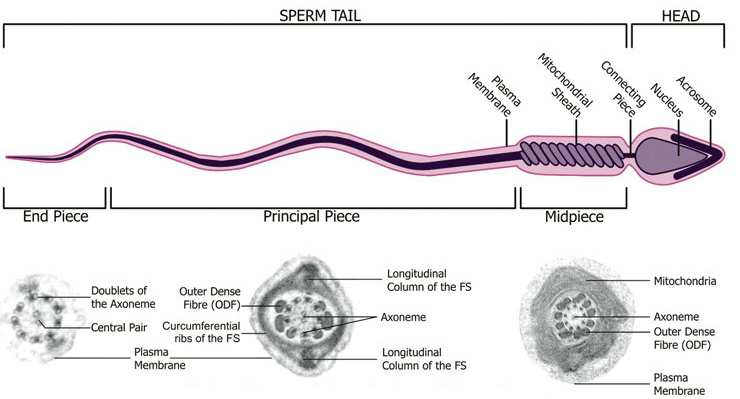
\includegraphics[scale=.55]{figure/sperm2} 

}

\caption[Structure du flagelle d’un spermatozoïde]{\textbf{\emph{Structure du flagelle d'un spermatozoïde}
d'après {[}\protect\hyperlink{ref-Borg2010}{45}{]}} : Coupes
transversales en microscopie électronique. Le flagelle se compose de
trois parties : la pièce intermédiaire, contenant les mitochondries, la
pièce principale et la pièce terminale. L'axonème, en position centrale,
parcours tout le flagelle. Des structures périaxonèmales sont
observables : les fibres denses dans la pièce intermédiaire et
principale, et la gaine fibreuse dans la pièce principale seulement.}\label{fig:flagelle}
\end{figure}










\newpage

\section{L'infertilité masculine}\label{linfertilite-masculine}

L'organisation mondiale de la santé définie l'infertilité comme étant :
``\emph{une pathologie du système reproductif définie par l'échec d'une
grossesse clinique après 12 mois ou plus de rapports sexuels réguliers
non protégés}''
(\href{http://www.who.int/reproductivehealth/topics/infertility/definitions/en/}{\texttt{Who.int.\ 2013-03-19.\ Retrieved\ 2013-06-17}}).
L'étude de l'infertilité représente un des enjeux scientifique et
médical majeur de ces dernières années. On estime qu'environ 10 à 15\%
des couples humains font face à des problèmes d'infertilité soit plus de
70 millions de personnes dans le monde
{[}\protect\hyperlink{ref-Boivin2007a}{46}{]}. Dans la moitié des cas,
la cause sous-jacente serait masculine. On estime que les facteurs
causaux sous-jacents de l'infertilité masculine peuvent être attribués à
des toxines environnementales, des troubles systémiques tels que la
maladie hypothalamo-hypophysaire, les cancers testiculaires et l'aplasie
des cellules germinales. Les facteurs génétiques, y compris les
aneuploïdies et les mutations de gènes uniques, contribuent également à
l'infertilité masculine. Cependant, aucune cause n'est identifiée dans
près de la moitié des cas. Comme nous avons pu le voir, la
spermatogenèse est une succession de processus complexes qui s'effectue
de manière coordonnée ; de fait la moindre altération génétique
affectant une seule de ces étapes est susceptible d'entraîner un
phénotype d'infertilité
{[}\protect\hyperlink{ref-Grudzinskas1995}{47}{]}.

\subsection{Les différents phénotypes d'infertilité
masculine}\label{les-differents-phenotypes-dinfertilite-masculine}

Chez l'homme, l'infertilité est associée à une altération quantitative
et / ou qualitative des spermatozoïdes présents dans l'éjaculat.
L'ensemble de ces altérations peut être détecté et quantifié dans des
laboratoires spécialisés, par réalisation d'un spermogramme. Au cours de
celui-ci, plusieurs critères tels que le volume de sperme sécrété, son
pH, la quantité et la vitalité des spermatozoïdes qu'il contient seront
évalués. La proportion de cellules immatures sera elle aussi analysée.
Ces cellules rondes, se retrouvent à la fois dans l'éjaculat des
individus ayant une quantité de spermatozoïdes ``normale''
{[}\protect\hyperlink{ref-Michael1937}{48}{]}, chez les individus
présentant une quantité basse de spermatozoïdes
{[}\protect\hyperlink{ref-MacLeod1970}{50},
\protect\hyperlink{ref-Tomlinson1993}{51}{]} ou en étant dépourvu
{[}\protect\hyperlink{ref-Kurilo}{52}{]}. Cependant, leur nombre
augmente tandis que la quantité de spermatozoïde diminue
{[}\protect\hyperlink{ref-SPERLING1971}{53}{]}.

\newpage

\subsubsection{Anomalies liées à la quantité
spermatique}\label{infquant}

Chez l'humain, l'arrêt de la spermatogenèse est défini comme
l'incapacité des cellules spermatogénétiques à devenir des
spermatozoïdes matures. Elle peut survenir à n'importe quelle étape de
la formation des cellules germinales. Les blocages méiotiques, au stade
de spermatocyte I, sont les plus fréquents, suivis par l'arrêt au niveau
des spermatides et moins fréquemment au niveau des spermatogonies
{[}\protect\hyperlink{ref-Girgis}{54}{]}.

\begin{enumerate}
\def\labelenumi{\arabic{enumi}.}
\item
  \textbf{L'oligozoospermie} : l'oligozoospermie est définie comme un
  phénotype d'infertilité masculine caractérisé par une production
  inférieure à 15 millions de spermatozoïdes par ml de sperme
  {[}\protect\hyperlink{ref-Cooper2010}{55}{]}. Un arrêt de la
  spermatogenèse a été observé dans 4 à 30\% des biopsies testiculaires
  des hommes présentant une oligospermie sévère
  {[}\protect\hyperlink{ref-Colgan1980}{56}--\protect\hyperlink{ref-WONG1973}{59}{]}.
  Cet arrêt a longtemps été considéré comme sans espoir pour les couples
  désirant concevoir, jusqu'à l'émergence de l'injection mécanique d'un
  spermatozoïde dans l'ovocyte appelé \emph{intracytoplasmic sperm
  injection} (ICSI) {[}\protect\hyperlink{ref-Palermo1992}{60}{]}.
\item
  \textbf{L'azoospermie} : comme l'oligozoospermie, l'azoospermie est un
  phénotype d'infertilité masculine cette fois-ci caractérisé par
  l'absence totale de spermatozoïdes dans l'éjaculat. On distingue des
  causes excrétoires empêchant l'excrétion des spermatozoïdes, on parle
  alors d'azoospermie obstructive et des causes sécrétoires, les plus
  fréquentes, accompagnées d'un défaut de la spermatogenèse, on parle
  alors d'azoospermie non-obstructive.
\end{enumerate}

\subsubsection{Anomalies liées à la
morphologie}\label{anomalies-liees-a-la-morphologie}

Ces anomalies sont observables en effectuant un spermocytogramme.
Plusieurs classifications ont été établies. Cependant, c'est la
classification de David modifiée (\textbf{Table :}
\ref{fig:anomaliemorphosperm}) qui est la plus répandue en France. Pour
ce faire, on procède généralement à une observation de 100
spermatozoïdes au cours de laquelle l'ensemble des anomalies observées
est relevé et quantifié permettant ainsi de définir un index d'anomalies
multiples (nombre total d'anomalies/nombre de spermatozoïdes anormaux)
révélant le nombre moyen d'anomalies par spermatozoïdes.

\newpage  

\begin{figure}

{\centering \includegraphics[scale=.75]{figure/tab_sperm_defect} 

}

\caption[Classification morphologique de spermatozoïdes humains normaux et anormaux]{\textbf{\emph{Classification morphologique de
spermatozoïdes humains normaux et anormaux} d'après
{[}\protect\hyperlink{ref-Auger2001}{61}{]}}.}\label{fig:anomaliemorphosperm}
\end{figure}





\newpage

\subsubsection{Anomalies liées à la
mobilité}\label{anomalies-liees-a-la-mobilite}

Le succès du passage du spermatozoïde le long du tractus génitale
féminin dépend en grande partie de la mobilité et de la vitesse du
spermatozoïde {[}\protect\hyperlink{ref-Lindholmer1974}{62},
\protect\hyperlink{ref-Bjorndahl2010}{63}{]}. La vitesse moyenne d'un
spermatozoïde étant de 25 \(\upmu\)m/s. Une mauvaise mobilité observée
dans plus de 50\% des spermatozoïdes éjaculés se révèle être un
prédicteur de l'échec de la fécondation
{[}\protect\hyperlink{ref-Aitken1985}{64}{]}.

\subsection{La génétique de
l'infertilité}\label{la-genetique-de-linfertilite}

Comme il a déjà été dit, il est estimé que 10 à 15\% des couples humains
font face à des problèmes d'infertilité. Par ailleurs, 30\% des
infertilités restent inexpliqués et près de 40\% ont des causes
incertaines. Ainsi, l'infertilité masculine d'origine génétique pourrait
concerner près d'un homme sur quarante
{[}\protect\hyperlink{ref-Tuttelmann2011}{65}{]}.

\subsubsection{Les causes fréquentes}\label{les-causes-frequentes}

\begin{enumerate}
\def\labelenumi{\arabic{enumi}.}
\tightlist
\item
  \textbf{Les microdélétions du chromosome Y} : le chromosome Y est un
  petit chromosome atteignant une taille d'environ 53 Mb. Il est porteur
  de 78 gènes principalement impliqués dans la différentiation sexuelle
  masculine et la spermatogenèse
  {[}\protect\hyperlink{ref-Skaletsky2003}{66}{]}. De fait, le
  chromosome Y représente une région d'intérêt évidente dans l'étude de
  facteurs génétiques liés à l'infertilité masculine. L'évolution des
  technologies a permis de mettre en évidence des délétions invisibles
  au caryotype dans la région du facteur AZF (\emph{Azoospermia
  Factor}). Cette région peut être subdivisée en trois sous-parties,
  AZFa, AZFb et AZFc (\textbf{Figure :} \ref{fig:chry}). Depuis
  plusieurs années, de nombreuses séries de patients azoospermiques ou
  oligozoospermiques ont été étudiées et publiées et tendent à montrer
  que les microdélétions du chromosome Y seraient responsables de 10\%
  des cas d'azoospermie non-obstructive et chez 5\% des cas
  d'oligozoospermie sévère (\textless{}5 millions de spermatozoïdes/ml)
  {[}\protect\hyperlink{ref-Hotaling2014}{67}{]}.
\end{enumerate}

\newpage

\begin{figure}

{\centering 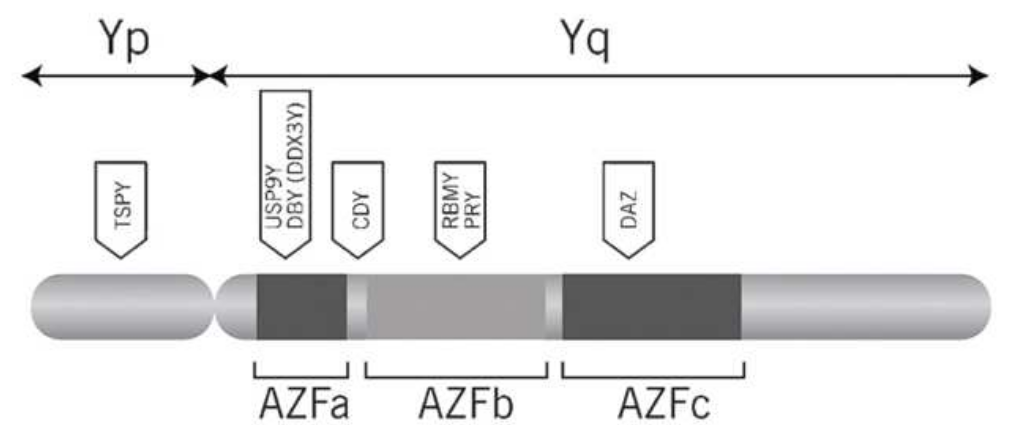
\includegraphics[scale=.45]{figure/chromozomeY} 

}

\caption[Représentation schématique du chromosome Y]{\textbf{\emph{Représentation schématique du chromosome Y}
adapté d'après {[}\protect\hyperlink{ref-OFlynnOBrien2010}{68}{]}} :
Visualisation la région AZF ainsi que des trois sous-régions AZF a, b, c
et des principaux gènes compris dans chacune des sous-régions.}\label{fig:chry}
\end{figure}






\begin{enumerate}
\def\labelenumi{\arabic{enumi}.}
\setcounter{enumi}{1}
\tightlist
\item
  \textbf{Anomalies chromosomiques} : des anomalies chromosomiques de
  nombre ou de structure impliquant les autosomes ou, le plus souvent,
  les gonosomes, peuvent être impliquées dans des cas d'infertilité
  masculine. Le pourcentage d'individus concernés varie entre 2 et 8\%
  et peut atteindre 15\% pour les patients azoospermiques soit 10 à 20
  fois la fréquence retrouvée dans la population générale
  {[}\protect\hyperlink{ref-Ravel2006}{69}{]}.

  \begin{enumerate}
  \def\labelenumii{\alph{enumii}.}
  \item
    \textbf{Syndrome de Klinefelter} : le syndrome de Klinefelter (ou
    46, XXY) fut décrit pour la première fois en 1942 par Harry F.
    Klinefelter. Il décrit une affection due à la présence d'un
    chromosome X supplémentaire suite à une erreur de ségrégation des
    chromosomes au moment de la méiose. Sa prévalence dans la population
    générale est estimée à environ 1 sur 1200 (1 homme sur 600)
    {[}\protect\hyperlink{ref-Bojesen2011}{70}{]} mais elle est environ
    50 fois supérieure chez les patients infertiles azoospermiques
    {[}\protect\hyperlink{ref-Gekas2001}{71}{]}.
  \item
    \textbf{Les anomalies de structure} : les translocations et les
    inversions sont les anomalies de structure retrouvées le plus
    fréquemment chez les patients infertiles.

    \begin{enumerate}
    \def\labelenumiii{\roman{enumiii}.}
    \tightlist
    \item
      La translocation est définie comme l'échange de matériel génétique
      entre deux chromosomes non homologues. On en distingue deux types,
      les translocations réciproques et les translocations
      robertsonniennes. Les premières (\textbf{Figure :}
      \ref{fig:figtranslocation} - \textbf{A}) décrivent un échange
      équilibré entre deux mêmes segments chromosomiques de deux
      chromosomes différents. Elles sont retrouvées 4 à 10 fois plus
      fréquemment chez les patients infertiles que dans la population
      générale {[}\protect\hyperlink{ref-Elliott1997}{72}{]}. Les
      secondes (\textbf{Figure :} \ref{fig:figtranslocation} -
      \textbf{B}) impliquent deux chromosomes acrocentriques et sont
      caractérisées par la fusion entre les brins longs de deux
      chromosomes, les brins courts étant perdus. Elles sont retrouvées
      chez 1.6\% des patients oligozoospermiques et 0.09\% des patients
      azoospermiques {[}\protect\hyperlink{ref-OFlynnOBrien2010}{68}{]}.
    \end{enumerate}
  \end{enumerate}
\end{enumerate}







\begin{figure}

{\centering \includegraphics[scale=.55]{figure/translocation} 

}

\caption[Les différents types de translocation]{\textbf{\emph{Les différents types de
translocation} d'après
\href{http://www.embryology.ch/francais/kchromaber/abweichende03.html}{embryology.ch}}
: \textbf{A} : La translocation réciproque. \textbf{B} : La
translocation robertsonniènne}\label{fig:figtranslocation}
\end{figure}

\begin{enumerate}
\def\labelenumi{\roman{enumi}.}
\setcounter{enumi}{1}
\item
  Les inversions chromosomiques caractérisent le mécanisme de cassure
  d'un fragment de chromosome suivi de son retournement à 180° et sa
  réintégration à la même position. Ces inversions vont gêner
  l'appariement des chromosomes homologues (formation d'une boucle
  d'inversion) pendant la méiose et sont, comme les translocations,
  retrouvées plus fréquemment chez les patients infertiles que dans la
  population générale {[}\protect\hyperlink{ref-Krausz2000}{73}{]}.

  \begin{enumerate}
  \def\labelenumii{\alph{enumii}.}
  \setcounter{enumii}{2}
  \tightlist
  \item
    \textbf{Autres anomalies chromosomiques} : parmi les anomalies
    chromosomiques responsables d'infertilité masculine, on peut par
    exemple citer les hommes de formule 46,XX. Ces patients sont
    généralement totalement infertiles et présentent une azoospermie par
    absence des sous- régions AZF a, b et c
    {[}\protect\hyperlink{ref-Vorona2007}{74}{]} bien qu'ils aient un
    phénotype masculin normal. Ces anomalies sont souvent le fait de la
    translocation du gène SRY sur un des chromosomes X du patient.
  \end{enumerate}
\end{enumerate}

\begin{enumerate}
\def\labelenumi{\arabic{enumi}.}
\setcounter{enumi}{2}
\tightlist
\item
  \textbf{Mutations du gène \emph{CFTR} }: l'identification du gène
  \emph{CFTR} (\emph{Cystic Fibrosis Transmembrane conductance
  Regulator}) chez les patients atteints de mucoviscidose et présentant
  une agénésie bilatérale des canaux déférents (ABCD) a permis
  d'associer ce gène au phénotype d'azoospermie obstructive. Cette
  malformation serait responsable de 2\% des cas d'infertilité masculine
  et de 25\% des cas d'azoospermie obstructive
  {[}\protect\hyperlink{ref-Yu2012}{75}{]}.
\end{enumerate}

Bien que la prévalence de ces anomalies génétiques varie en fonction du
phénotype concerné, il est estimé que ces défauts sont seulement
retrouvés chez 5\% des cas d'infertilité masculine, tous phénotypes
confondus. Cette observation suggère fortement l'implication de nombreux
autres gènes encore inconnus dans les différents phénotypes
d'infertilité masculine.

\newpage

\subsubsection{Les nouveaux gènes}\label{les-nouveaux-genes}

\begin{enumerate}
\def\labelenumi{\arabic{enumi}.}
\item
  \textbf{Les anomalies quantitatives} : une analyse de trois familles
  par séquençage \protect\hyperlink{ngs}{haut-débit} a permis
  d'identifier trois gènes \emph{MEIOB}, \emph{TEX14} et \emph{DNAH6}
  impliqués dans un phénotype d'azoospermie ; de même une étude de 2016
  démontre l'association de trois variants dans la séquence codante du
  gène \emph{RAD21L} en se basant sur une étude statistique effectuée
  sur 38 japonais présentant un arrêt de la fertilité et 200 contrôles
  {[}\protect\hyperlink{ref-Minase2017}{76}{]}. De même, plusieurs
  variants dans le gène \emph{TEX111} et \emph{SYC1} ont été décrits
  comme entrainant un arrêt de la méiose
  {[}\protect\hyperlink{ref-Yatsenko2015}{77}--\protect\hyperlink{ref-Maor-Sagie2015}{79}{]}.
\item
  \textbf{Les anomalies morphologiques liées à la tête du spermatozoïde}
  :

  \begin{enumerate}
  \def\labelenumii{\alph{enumii}.}
  \tightlist
  \item
    \textbf{La macrozoospermie} : Ce phénotype d'infertilité masculine
    rare est caractérisé par la présence de 100\% des spermatozoïdes de
    l'éjaculat présentant une tête anormalement grosse ainsi que
    plusieurs flagelles. Il fut observé pour la première fois en 1978
    {[}\protect\hyperlink{ref-Nistal}{80}{]}, mais ce n'est qu'en 2007
    qu'une explication génétique fut enfin trouvée. Une étude portant
    sur 14 patients nord-africains a permis d'identifier la délétion
    c144delC du gène \emph{AURKC} (\emph{Aurora kinase C}) comme
    responsable du phénotype de l'ensemble des individus de l'étude
    {[}\protect\hyperlink{ref-Dieterich2007}{81}{]}. Depuis, d'autres
    études ont permis d'associer d'autres variants sur ce même gène à ce
    phénotype {[}\protect\hyperlink{ref-BenKhelifa2011}{82}{]}. Des
    anomalies du gène \emph{AURKC} seraient ainsi responsables d'environ
    83.7\% des cas macrozoospermie chez des patients non apparentés
    {[}\protect\hyperlink{ref-Dieterich2007}{81}{]}. Le gène AURKC,
    étant impliqué dans la méiose, conduit lorsqu'il est muté à un
    blocage de la première division méiotique, entraînant la production
    de spermatozoïdes tétraploïdes, c'est à dire, portant une quantité
    de matériel génétique quatre fois supérieure à la normale
    {[}\protect\hyperlink{ref-Dieterich2009}{83}{]}.\\
  \item
    \textbf{La globozoospermie} : La globozoospermie est aussi un
    phénotype rare d'infertilité dont la prévalence est estimée à de
    0,1\%. Il fut identifié pour la première fois en 1971 et est
    caractérisé par la présence dans l'éjaculat d'une majorité de
    spermatozoïdes dépourvus d'acrosome, empêchant le spermatozoïde de
    franchir la zone pellucide de l'ovocyte et compromettant ainsi la
    fécondation
    {[}\protect\hyperlink{ref-Dam2006}{84}--\protect\hyperlink{ref-Holstein1973}{86}{]}.
    En 2007, une étude familiale a permis de lier ce phénotype à la
    mutation c.848G\textgreater{}A dans le gène \emph{SPATA16}
    (\emph{spermatogenesis-associated protein 16})
    {[}\protect\hyperlink{ref-Dam2007a}{87}{]} dont la protéine va, au
    cours de la spermatogenèse, fusionner avec les vésicules
    proacrosomales pour former l'acrosome
    {[}\protect\hyperlink{ref-Dam2007a}{87},
    \protect\hyperlink{ref-Lu2006}{88}{]}. Plus tard, en 2011, une étude
    portant sur 20 patients tunisiens permit d'identifier une délétion
    homozygote de 200 kb emportant la totalité du gène \emph{DPY19L2}
    (\emph{Dpy-19 Like 2}) chez 15 des 20 patients
    {[}\protect\hyperlink{ref-Harbuz2011}{89}{]}. cf
    \protect\hyperlink{globo}{globo}\\
  \item
    \textbf{Spermatozoïdes acéphaliques} : Ce phénotype rapporté
    plusieurs fois
    {[}\protect\hyperlink{ref-Chemes2010}{90}--\protect\hyperlink{ref-Chemes1987}{92}{]}
    caractérise les patients présentant des spermatozoïdes dépourvus de
    tête dans leur éjaculat. Une étude récente a pu lier ce phénotype à
    une mutation c.824C\textgreater{}T homozygote ainsi qu'à deux
    variants hétérozygotes composites c.1006C\textgreater{}T et
    c.485T\textgreater{}A dans le gène \emph{SUN5}
    {[}\protect\hyperlink{ref-Zhu2016}{93}{]} qui avait précédemment été
    décrit comme localisant à la jonction noyau / flagelle du
    spermatozoïde {[}\protect\hyperlink{ref-Yassine2015}{94}{]}.
  \end{enumerate}
\item
  \textbf{Le phénotype MMAF} : Le phénotype MMAF (\emph{Multiple
  morphological abnormalities of the sperm flagella}) décrit les
  patients atteints d'asthenozoospermie dont les spermatozoïdes
  présentent de multiples anomalies morphologiques touchant en
  particulier les flagelles. Plus précisément, ce phénotype décrit les
  asthenozoospermie résultant d'une mosaïque d'anomalies morphologiques
  au niveau du flagelle tel que l'absence totale de flagelle, des
  flagelles enroulés, courts, anguleux\ldots{}
  {[}\protect\hyperlink{ref-Coutton2015}{95},
  \protect\hyperlink{ref-BenKhelifa2014}{96}{]}. Récemment, le gène
  \emph{DNAH1} (\emph{Dynein Axonemal Heavy Chain 1}) codant pour une
  dynéine de la chaine lourde de l'axonème a été retrouvé muté chez près
  d'un patient sur trois dans sa cohorte comportant 18 patients
  {[}\protect\hyperlink{ref-BenKhelifa2014}{96}{]}. Deux autres études
  ont retrouvé des mutations dans le gène \emph{DNAH1} chez des patients
  venant de Chine, d'Iran et d'Italie, laissant suggérer que ce gène est
  l'un des acteurs majeurs dans le syndrome MMAF
  {[}\protect\hyperlink{ref-Wang2017}{97},
  \protect\hyperlink{ref-Amiri-Yekta2016}{98}{]}.
\item
  \textbf{Les échecs de fécondation du spermatozoïde} : Au moment de la
  fécondation, l'activation ovocytaire repose sur le relargage par le
  spermatozoïde de ``facteurs spermatiques'' qui déclenchent un signal
  de calcium, constitué d'oscillations Ca\textsuperscript{2+}. Ce
  processus est médié par une protéine spécifique du spermatozoïde,
  \emph{la phospholipase C Zeta 1} (PLC\(\zeta 1\)) codée par le gène
  \emph{PLCZ1} {[}\protect\hyperlink{ref-Nomikos2013}{99},
  \protect\hyperlink{ref-Amdani2013}{100}{]}. Plusieurs cas d'échec
  d'activation ovocytaire ont été liés à l'absence ou à la mauvaise
  localisation de la protéine PLC\(\zeta1\). Malgré cela, aucune preuve
  génétique directe n'avait été reportée jusqu'à récemment où deux
  mutations au sein du gène \emph{PLC}\(\zeta\)\emph{1} furent
  retrouvées chez un patient
  {[}\protect\hyperlink{ref-Heytens2009}{101}{]} et un peu plus tard une
  mutation homozygote chez deux frères consanguins
  {[}\protect\hyperlink{ref-Escoffier2016}{102}{]}.
\end{enumerate}

\newpage  

\section{Les techniques d'analyses
génétiques}\label{les-techniques-danalyses-genetiques}

L'acide désoxyribonucléique (ADN) a été identifié comme étant le porteur
de l'information génétique par Oswald Theodore Avery en 1944. Sa
structure en double hélice composée par quatre bases, la thymine (T),
l'adénine (A), la guanine (G) et la cytosine (C) fut caractérisée en
1953 par James D. Watson et Francis Crick. Cependant, l'existence
``d'entités d'information génétiques discrètes'' que sont les gènes fut
suggéré dès la deuxième moitié du XIX\textsuperscript{ième} siècle grâce
aux travaux de Gregor Mendel portant sur l'hérédité de certains traits
chez le pois. Depuis, de nombreuses méthodes permettant de lier le
phénotype d'un individu à son génotype ont vu le jour au gré des
améliorations technologiques.

\subsection{\texorpdfstring{Approche ``gènes
candidats''}{Approche gènes candidats}}\label{approche-genes-candidats}

L'approche ``gènes candidats''" consiste à rechercher des mutations chez
un patient dans un ou plusieurs gènes cibles. Le choix des gènes cibles
se fera en fonction de plusieurs critères. Le premier d'entre eux est
l'étude de gènes reliés à des phénotypes proches du phénotype étudié
dans différents modèles animaux et notamment murins. Dans ce cas, les
mutations seront recherchées sur le gène orthologue humain
{[}\protect\hyperlink{ref-DeBoer2015}{103}{]}. Une autre possibilité
consiste à rechercher des variants dans des gènes paralogues à un gène
précédemment identifié avec l'idée sous-jacente que leur structure
proche implique une fonction similaire. Enfin la dernière méthode
consiste à étudier des gènes connus comme étant des partenaires de gènes
déjà identifiés dans cette pathologie, en supposant que si un variant
dans un gène donné entraîne une pathologie, un variant dans un
partenaire de ce gène pourrait entraîner le même phénotype. Cette
approche est bien souvent infructueuse, ceci étant dû, en grande partie,
à l'hétérogénéité génétique des phénotypes étudiés, au nombre limité de
patients testés {[}\protect\hyperlink{ref-ElInati2012}{104}{]} et aux
connaissances souvent incomplètes sur le phénotype. De fait, cette
approche a quasiment disparu au profit des méthodes à haut débit que
sont les puces et le séquençage nouvelle génération (NGS). Néanmoins,
cette méthode compte à son actif plusieurs succès retentissants avec
dans le domaine de l'infertilité masculine, les gènes \emph{SYCP3},
\emph{SOHLH1} et \emph{NR5A1} entraînant tous les trois un phénotype
d'azoospermie
{[}\protect\hyperlink{ref-Miyamoto2003}{105}--\protect\hyperlink{ref-Bashamboo2010}{107}{]}.

\newpage

\subsection{Les puces}\label{les-puces}

Les puces à ADN furent initialement conçues dans le but de mesurer le
niveau de transcription des transcrits provenant de plusieurs milliers
de gènes lors d'une seule et unique expérience. Cette technologie a
ainsi permis de déterminer des patterns d'expression de gènes à un statu
physiologique donné. L'analyse des ``signatures'' d'expression a ainsi
permis de caractériser plusieurs cancers
{[}\protect\hyperlink{ref-Alon1999}{108}--\protect\hyperlink{ref-VantVeer2002}{111}{]},
mais aussi la réponse physiologique à plusieurs types de stimuli tel que
la prise de certains médicaments
{[}\protect\hyperlink{ref-Brachat2002}{112}{]}.

Suite à cela, l'usage des puces à ADN dans le domaine biomédical s'est
étendu pour ne plus être limité à la simple quantification de
l'expression génique. Ainsi, cette technologie a également été utilisée
afin de détecter des \emph{single nucleotide polymorphisms} (SNPs) au
sein de notre génome permettant notamment l'émergence du HapMap Project
qui recense les SNPs de plusieurs milliers d'individus
{[}\protect\hyperlink{ref-Cutler2001}{113}{]}. De même, l'utilisation
des puces à ADN a permis la détection de \emph{copy number variation}
(CNVs).

Pendant plus de 10 ans, la grande qualité des puces, l'existence de
protocoles d'hybridation standardisés ainsi que des algorithmes
d'analyses robustes ont fait des puces à ADN l'outil d'analyse génomique
le plus puissant avant l'arrivée du \protect\hyperlink{ngs}{séquençage
haut débit}

\newpage

\subsubsection{Les puces à expression}\label{les-puces-a-expression}

L'utilisation principale des puces à ADN a été de mesurer l'expression
des gènes dans un tissus donné. Dans cette application, l'ARN est
extrait des cellules d'intérêt puis est généralement converti en ADNc.
Dans un second temps, l'ADNc est hybridé à la puce qui subira par la
suite une étape de lavage. Pour finir, l'intensité de fluorescence est
mesurée à chaque spot de la puce et déterminera le niveau d'expression
d'un gène.

\begin{figure}

{\centering \includegraphics[scale=.9]{figure/expression_array} 

}

\caption[Représentation schématique des méthodes d'analyse d'expression génique par puce à ADN]{\textbf{\emph{Représentation schématique des méthodes
d'analyse d'expression génique par puce à ADN} d'après
{[}\protect\hyperlink{ref-Trevino2007}{114}{]}} : Présentation des
méthodes à double et à simple colorant, respectivement à gauche et à
droite. Pour les analyses à double colorant, une seule puce et
nécessaire, les échantillons de la référence et du test sont mis en
compétition sur la même puce, un signal de sortie vert indiquera une
surexpression chez le test tandis qu'un signal rouge indiquera une
sous-expression. Pour celles à simple colorant, deux puces sont
nécessaires, une première pour la référence et une seconde pour le test.
Les données des deux puces sont ensuite comparées pour déterminer quels
sont les gènes différentiellement exprimés. Dans le cas de la CGH array,
le principe est similaire, en remplaçant simplement l'ARNm par de
l'ADNg.}\label{fig:pictexparray}
\end{figure}
















\newpage

\subsubsection{Les puces à SNP, plateforme
génotypage}\label{les-puces-a-snp-plateforme-genotypage}

Bien que leur utilité principale ait été d'analyser l'expression des
gènes, les puces à ADN ont également été extrêmement utilisées comme
moyen de génotyper les SNP (\emph{single-nucleotide-polymorphism}). De
nombreuses méthodes ont été mises en place pour cela ; cependant la plus
employée est la méthode de discrimination allélique par hybridation
telle qu'elle est utilisée par Affymetrix
{[}\protect\hyperlink{ref-Wang1998}{115}{]} malgré le ``bruit de fond''
causé par l'hybridation non spécifique dont elle souffre (\textbf{Figure
:} \ref{fig:pictallelicdisc}).

\begin{figure}

{\centering \includegraphics[scale=.7]{figure/allelic_discrimination} 

}

\caption[Méthode de génotypage par discrimination allélique par hybridation]{\textbf{\emph{Méthode de génotypage par
discrimination allélique par hybridation} d'après
{[}\protect\hyperlink{ref-Bumgarner2013}{116}{]}} : Des sondes
complémentaires à chacun des allèles sont positionnées sur la puce.
L'ADN génomique fragmenté et labélisé est mis en contact de la puce.
Après nettoyage de la puce, l'analyse du signal émis par l'ADN génomique
permettra de déterminer si l'individu est homozygote pour cette allèle
(hybridation à une seule des deux sondes) ou bien hétérozygote pour
cette allèle (hybridation aux deux sondes).}\label{fig:pictallelicdisc}
\end{figure}











\newpage

\subsubsection{Les puces à indels}\label{les-puces-a-indels}

L'implication de réarrangements génomiques tel que des duplications,
translocations ou délétions dans divers pathologies est bien connue.
C'est afin de détecter ces réarrangements que la \emph{Comparative
Genomic Hybridization array} (CGH array) a été développée dès 1999
{[}\protect\hyperlink{ref-Brown1999}{117}{]}. Son principe est très
similaire à celui utilisé dans les puces à expression (\textbf{Figure :}
\ref{fig:pictexparray}) en remplaçant simplement l'ARN messager (ARNm)
par de l'ADN génomique (ADNg). Ainsi, la présence d'un CNV sera
facilement détectée en comparant le signal émis par un individu test
avec celui émis par un contrôle.

\subsubsection{Limitation}\label{limitation}

Bien que cette technologie ait été largement utilisée dans divers champs
d'applications, elle présente deux limitations principales.

\begin{enumerate}
\def\labelenumi{\arabic{enumi}.}
\item
  \textbf{Limitation n°1 :} Pour les génomes complexes (tel que les
  mammifères), il est difficile, si ce n'est impossible de
  \emph{designer} une puce ne permettant pas de l'hybridation non
  spécifique. En effet, la séquence d'une puce prévue pour détecter le
  gène ``A'' pourra également détecter les gènes ``B'', ``C'' et ``D''
  si ceux-ci présentent une forte homologie avec ``A'' Ce qui est
  particulièrement problématique dans le cas d'analyse de gènes d'une
  même famille.
\item
  \textbf{Limitation n°2 :} les puces détectent uniquement ce pour quoi
  elles ont été \emph{designer}. Ainsi, si la solution que l'on hybride
  sur la puce contient des séquences d'ADN ou d'ARN pour lesquelles il
  n'y a aucune sonde complémentaire sur la puce, celles-ci ne seront pas
  détectées. Cela peut avoir de grandes répercutions puisque par exemple
  dans le cas des puces à expression, les gènes qui n'ont pas encore été
  annotés risquent de ne pas être représentés sur la puce.
\end{enumerate}

\newpage

\hypertarget{ngs}{\subsection{Le séquençage NGS}\label{ngs}}

Le terme séquençage de l'ADN fait référence à l'ensemble des techniques
permettant de déterminer l'ordre des nucléotides A, T, C et G de
l'intégralité ou d'une partie d'une molécule d'ADN. Avant de parler des
nouvelles technologies de séquençage (NGS) faisons un bref historique du
séquençage de l'ADN. En 1977 Frederick Sanger développe une technologie
de séquençage d'ADN basée sur la méthode \emph{chain-termination}. Ce
procédé est désormais connu sous le nom de séquençage Sanger. D'autres
méthodes furent développées à la même période, notamment celle de Walter
Gilbert basée sur la modification chimique de l'ADN, cependant sa grande
efficience et sa faible utilisation de la radioactivité permirent au
séquençage Sanger de s'imposer comme référence dans la ``première
génération'' de séquenceur à application commerciale et de recherche.
Apparus en 1998, les instruments de séquençage automatique ainsi que les
logiciels associés utilisant le séquençage par capillarité et la
technologie Sanger furent les outils principaux qui permirent la
complétion du \emph{human genome project} en 2001
{[}\protect\hyperlink{ref-Collins2003}{118}{]}.

Contrairement à la méthode Sanger, le NGS est capable de ``\emph{lire}''
des fragments d'ADN provenant d'un génome \textbf{entier}. On parle
alors de séquençage de génomes entiers ou \emph{whole genome sequencing}
(WGS). Pour cela, la molécule d'ADN est ``coupée'' en plusieurs
fragments d'une taille donnée. Ce sont ensuite ces fragments qui seront,
après une étape d'amplification spécifique aux différentes plateformes,
séquencés simultanément. C'est pourquoi on parle souvent de séquençage
parallèle massif pour décrire le NGS. Le produit de ce séquençage est
appelé \emph{read}. Cette technologie est avantageuse de par la masse de
\emph{reads} qu'elle produit et par son faible coût par base séquencée
{[}\protect\hyperlink{ref-Metzker2010}{119}{]}. Ces caractéristiques ont
permis au séquençage Haut-débit d'être couramment utilisé dans le
domaine de la recherche clinique.

La taille des \emph{reads} obtenus par séquençage NGS est, hormis dans
le cas de la technologie PacBio, nettement inférieure à celle atteinte
par le séquençage Sanger. À l'heure actuelle, les \emph{reads} obtenus
par séquençage NGS ont une taille comprise entre 50 et 500 pb pour la
plupart des plateforme contre une taille d'environ 800 nucléotides
obtenus par Sanger (\textbf{Figure :} \ref{fig:pictreadPerRun}) ; c'est
pour cela que les résultats du séquençage NGS sont appelés des
\emph{reads} courts ou \emph{short reads}.\\
Étant donné que le NGS produit à l'heure actuelle des \emph{reads}
courts la notion de couverture est importante et représente l'un des
critères majeur à considérer dans l'analyse des données
{[}\protect\hyperlink{ref-Sims2014}{120}{]}. La couverture est définie
comme le nombre de \emph{reads} qui, après l'étape
\protect\hyperlink{lalignement}{d'alignement}, se chevauchent les uns
les autres au sein d'une région génomique spécifique. Par exemple, une
couverture de 30x pour le gène XXXX signifie que chaque nucléotide de ce
gène est chevauché par au moins 30 \emph{reads} distincts.

\newpage

\begin{figure}

{\centering 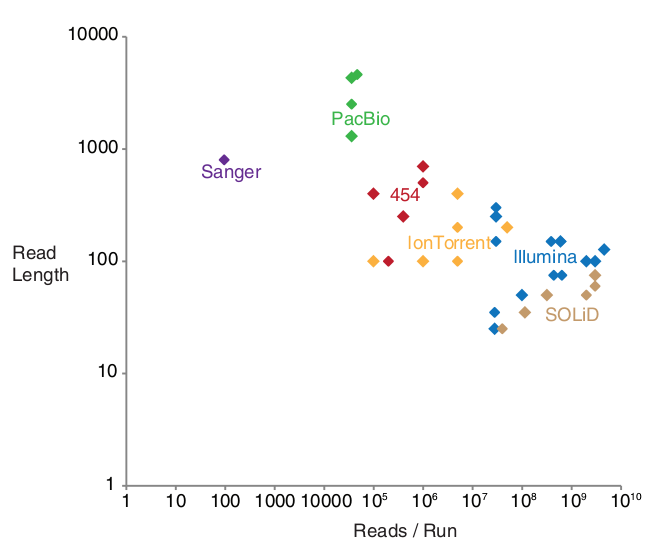
\includegraphics[scale=.55]{figure/read_per_run} 

}

\caption[Présentation de la taille des reads et du nombre de reads par run en fonction de la technologie de séquençage utilisée]{\textbf{\emph{Présentation de la taille des reads
et du nombre de reads par run en fonction de la technologie de
séquençage utilisée} d'après
{[}\protect\hyperlink{ref-Hodkinson2015}{121}{]}} : Chaque point
représente une plateforme de séquençage, la couleur détermine la marque
du séquenceur.}\label{fig:pictreadPerRun}
\end{figure}








\subsubsection{La capture des parties à séquencer, avantages et
inconvénients}\label{la-capture-des-parties-a-sequencer-avantages-et-inconvenients}

Pour de nombreuses applications, il peut être intéressant de ne
séquencer qu'une partie du génome et non pas son intégralité. Dans cette
sous partie de génome ciblé on peut trouver par exemple : une région
génomique spécifique à laquelle une pathologie a déjà été associée,
l'ensemble des exons de certains gènes candidats, ou encore
l'intégralité des exons de l'ensemble des gènes codant pour une
protéine. Dans ce dernier cas, on parle alors de séquençage exomique ou
\emph{whole exome sequencing} (WES). Les principaux avantages du WES par
rapport au WGS sont son coût réduit ainsi qu'une masse de données moins
importante à stocker et à analyser. En effet, l'ensemble de l'exome ne
représente qu'environ 1\% du génome entier. On considère cependant que
ces parties codantes contiennent plus de 90\% des anomalies responsables
de pathologies génétiques chez l'homme. Pour ces raisons, le WES est
considéré comme le standard dans le cadre de recherche sur des
pathologies génétiques et se révèle être un outil puissant pour
l'identification de variants associés à des pathologies
{[}\protect\hyperlink{ref-Ng2010}{122}{]}. Le procédé de séquençage est
identique au WGS, il est simplement précédé d'une étape d'enrichissement
au cours de laquelle les exons sont capturés par hybridation à des
sondes. De fait les exons capturés sont donc dépendants du kit de
capture utilisé, cette technique permet donc de séquencer uniquement les
exons connus et ciblés par les sondes. Il faut également noter que
depuis quelques années, plusieurs études ont remis en cause l'intérêt du
WES au profit du WGS, notamment car dans des conditions de séquençage
standards, la proportion des régions codantes, définies à la fois par
RefSeq et Ensembl, séquencée est plus importante dans le cas du WGS que
dans le WES {[}\protect\hyperlink{ref-Lelieveld2015}{123},
\protect\hyperlink{ref-Meienberg2016}{124}{]}. De plus le WES montre une
plus grande sensibilité au pourcentage de GC contenu dans la région à
séquencer et à la sélection des kits de capture utilisés
{[}\protect\hyperlink{ref-Meienberg2016}{124}{]}. Ainsi, bien que le WES
soit encore à l'heure actuelle le choix privilégié dans la majorité des
études, la réduction des coûts de séquençage et du stockage des données,
pourrait permettre prochainement au WGS de remplacer totalement le WES
ainsi que l'ensemble des techniques impliquant la capture de séquences
ciblées {[}\protect\hyperlink{ref-Meienberg2016}{124}{]}.

\subsubsection{L'amplification}\label{lamplification}

Dans la plupart des technologies, la phase de séquençage est précédée
par une étape d'amplification de l'ADN. Cette amplification se fait dans
la grande majorité des cas sur une surface solide excepté pour la PCR en
émulsion qui s'effectue en phase aqueuse. Elle permet d'obtenir dans une
région définie plusieurs milliers de copies du même fragment d'ADN,
appelés des clones. Cette étape assure que le signal émis lors du
séquençage pourra être distingué du bruit. Chacun de ces \emph{spots}
d'amplification appelés aussi centre de réaction, se retrouve donc être
le représentant d'un unique fragment d'ADN. Ceux-ci seront ensuite
séquencés parallèlement aux autres \emph{spots}. Une plateforme de
séquençage peut gérer plusieurs millions de ces centres de réactions
simultanément, séquençant ainsi plusieurs millions de molécules d'ADN en
parallèle, donnant ainsi le nom de séquençage massif en parallèle à ces
techniques. Cette étape d'amplification est généralement précédée d'une
phase de fragmentation de l'ADN. Cette fragmentation peut être physique,
enzymatique ou bien chimique. Ce sont les résidus d'ADN résultant de
cette fragmentation qui seront ensuite amplifiés. Il existe quatre
stratégies utilisées pour le clonage de l'ADN dans le cadre du NGS :

\begin{enumerate}
\def\labelenumi{\arabic{enumi}.}
\item
  \textbf{La PCR en émulsion ou emPCR} (\textbf{Figure :
  }\ref{fig:pictngsampli} - \textbf{a}) : Le patron d'ADN fragmenté
  simple brin est lié à une séquence adaptatrice complémentaire. Il est
  capturé par une gouttelette aqueuse appelée micelle contenant une
  bille recouverte d'adaptateur complémentaire à celui fixé sur le
  fragment d'ADN ainsi que tous les composants nécessaires à la réaction
  de PCR. En respectant un ratio nombre de molécules d'ADN / nombre de
  billes, on va fixer un seul fragment d'ADN sur chaque bille. Chacune
  de ces billes sera donc, en fin de réaction, recouverte par plusieurs
  milliers de copies de la même séquence d'ADN.
\item
  \textbf{L'amplification par pont sur face solide} (\textbf{Figure :
  }\ref{fig:pictngsampli} - \textbf{b}) : Les fragments d'ADN sont liés
  à des séquences adaptatrices et liés par une de leurs extrémités à une
  amorce fixée sur un support solide. Du fait de la dilution, les
  molécules d'ADN se trouvent éloignées les unes des autres. L'extrémité
  libre du fragment interagit avec les amorces situées à proximité
  formant une structure en pont, d'où le nom de PCR en pont ou
  \emph{bridge-PCR}. La PCR va alors synthétiser un deuxième brin
  complémentaire aux fragments immobilisés sur le support. En procédant
  à des cycles de température comme pour une réaction PCR classique, on
  obtient à l'emplacement de chaque molécule d'ADN un massif de
  molécules fixé sur la plaque, toutes identiques à la molécule
  initiale.
\item
  \textbf{Amplification par modèle mobile ou \emph{walking-template}
  }(\textbf{Figure : }\ref{fig:pictngsampli} - \textbf{c}) : L'ADN
  fragmenté est lié à un adaptateur et à une amorce complémentaire fixée
  sur un support solide. Le brin complémentaire du fragment sera
  synthétisé par PCR à partir de l'amorce fixée. La molécule double brin
  nouvellement formée sera ensuite partiellement dénaturée permettant à
  l'extrémité libre de se fixer à une séquence amorce voisine. Des
  amorces \emph{reverse} sont ensuite utilisées pour resynthétiser un
  fragment d'ADN libre à partir des fragments fixés sur le support.
\end{enumerate}

\newpage 

\begin{figure}

{\centering 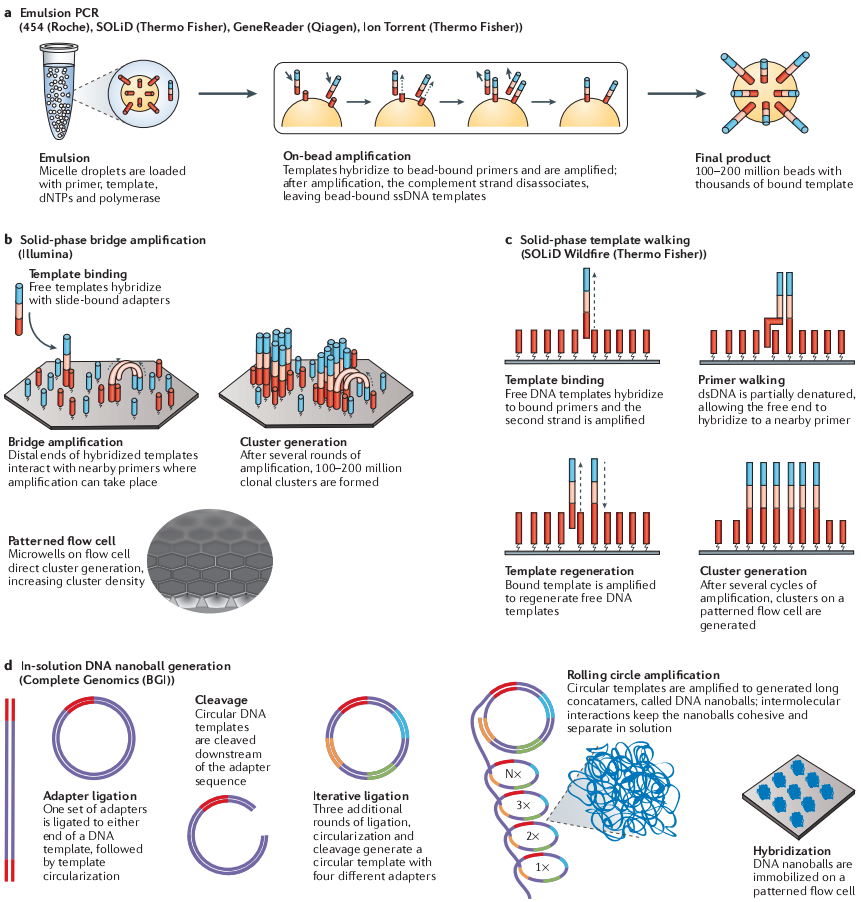
\includegraphics[scale=.5]{figure/ngs_amplification} 

}

\caption[Présentation des différentes stratégies d'amplification de l'ADN dans le cadre du NGS]{\textbf{\emph{Présentation des différentes stratégies
d'amplification de l'ADN dans le cadre du NGS} d'après
{[}\protect\hyperlink{ref-Goodwin2016}{125}{]}} : \textbf{a} : PCR en
émulsion. \textbf{b} : amplification par pont. \textbf{c} :
amplification par modèle mobile.}\label{fig:pictngsampli}
\end{figure}







\newpage

\subsubsection{La réaction de séquence}\label{la-reaction-de-sequence}

La réaction de séquence est l'étape suivant l'amplification. Elle
consiste à déterminer l'ordre dans lequel se succèdent les nucléotides
de l'ensemble des clones générés dans la phase d'amplification. Il
existe deux technologies principales permettant le séquençage de
\emph{reads} courts :

\begin{enumerate}
\def\labelenumi{\arabic{enumi}.}
\tightlist
\item
  \textbf{Séquençage par synthèse} (SBS) : Ce type de séquençage
  regroupe l'ensemble des méthodes utilisant l'ADN polymérase pour
  synthétiser de l'ADN. En 2016, Sahra Goodwin et ses collègues ont
  différenciés deux catégories de séquençage par synthèse
  {[}\protect\hyperlink{ref-Goodwin2016}{125}{]} :

  \begin{enumerate}
  \def\labelenumii{\alph{enumii}.}
  \tightlist
  \item
    \textbf{Terminaison par cycle réversible}, \emph{cyclic reversible
    termination} (CRT) (\textbf{Figure : }\ref{fig:pictcrtSeq}) : Cette
    méthode est caractérisée par l'utilisation de molécule dites
    terminatrices auxquelles le groupement \(\mathrm{3'-OH}\) est
    modifié de sorte à éviter l'élongation
    {[}\protect\hyperlink{ref-Guo2008}{126}{]}, on parlera de groupement
    \(\mathrm{3'-bloqué}\). Une amorce liée au fragment d'ADN permettra
    l'initialisation du processus de polymérisation. À chaque cycle, un
    mix comprenant l'ensemble des quatre désoxynucléotides (dNTPs),
    préalablement labélisés par un fluorophore \(\mathrm{3'-bloqué}\),
    est mis en contact du fragment. Après l'incorporation d'un unique
    dNTP au fragment, les dNTPs non liés sont éliminés et la nature du
    dNTP ajouté est identifiée grâce à son fluorophore. Le fluorophore
    et le groupement \(\mathrm{3'-bloqué}\) sont retirés permettant
    ainsi à un nouveau cycle de commencer.
  \end{enumerate}
\end{enumerate}

\begin{figure}

{\centering 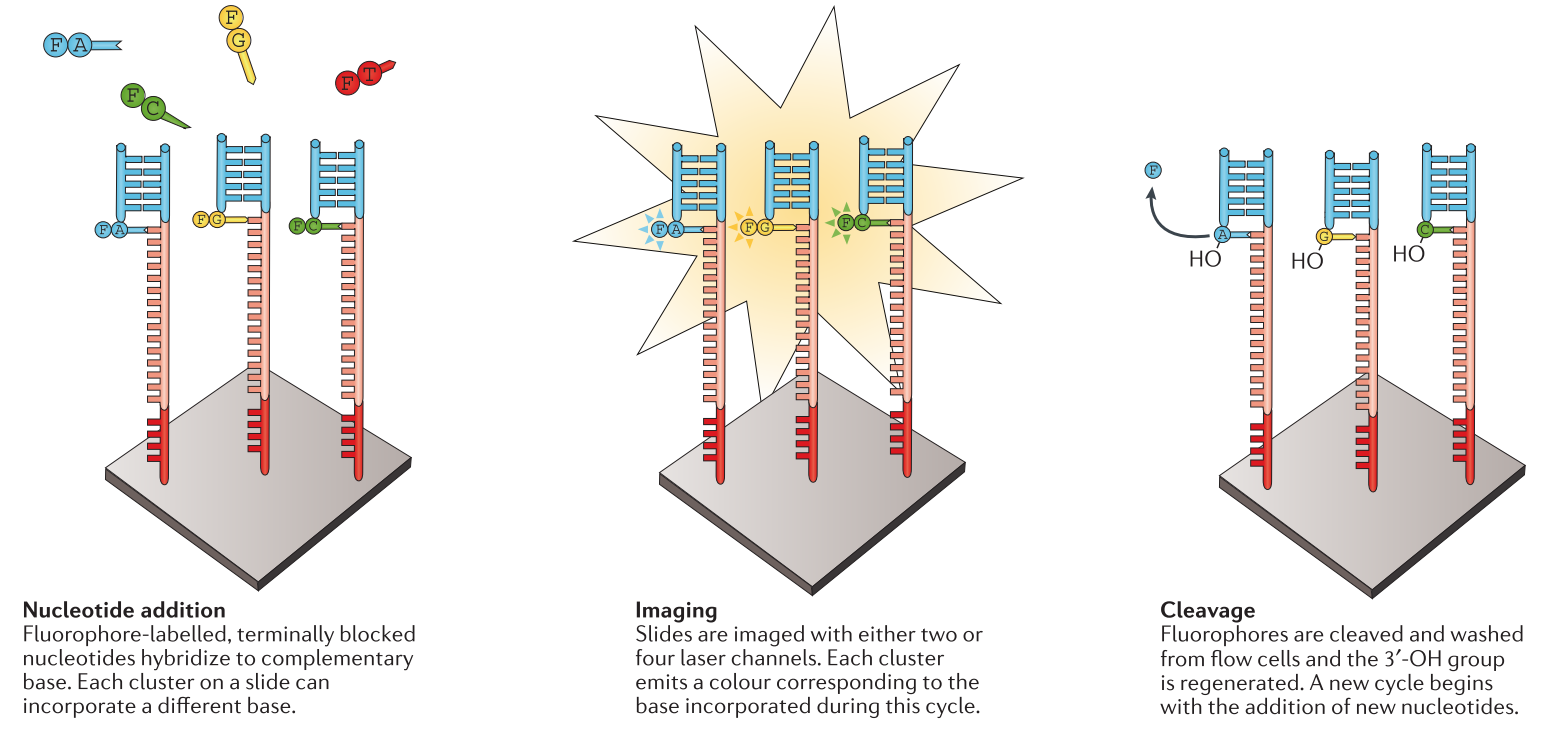
\includegraphics[scale=.24]{figure/CRT_seq_illumina} 

}

\caption[Séquençage CRT tel qu'il est effectué par Illumina]{\textbf{\emph{Séquençage CRT tel qu'il est effectué par
Illumina} d'après {[}\protect\hyperlink{ref-Goodwin2016}{125}{]}} :
\textbf{a} : ajout d'un dNTP labellisé par un fluorophore 3'-bloqué.
\textbf{b} : identification du dNTP ajouté grâce au fluorophore.
\textbf{c} : le fluorophore est clivé du dNTP et le groupement 3'-OH est
reformé à partir du groupement 3'-bloqué permettant ainsi l'élongation.}\label{fig:pictcrtSeq}
\end{figure}








\newpage

\begin{enumerate}
\def\labelenumi{\alph{enumi}.}
\setcounter{enumi}{1}
\tightlist
\item
  \textbf{Addition de nucléotides uniques} (SNA) (\textbf{Figure :
  }\ref{fig:pictsnaSeq}) : l'initialisation de la méthode SNA est
  identique à celle de la méthode CRT. La différence se fait donc au
  moment de la phase d'élongation. Contrairement à la méthode CRT, le
  mix contenant les dNTPs ne contient qu'un seul type de dNTP. Quatre
  mixs différents sont donc présentés successivement au fragment d'ADN à
  séquencer, ceux-ci se fixeront uniquement s'ils sont complémentaires à
  la séquence. Ces dNTPs n'ont donc pas besoin d'être
  \(\mathrm{3'-bloqué}\) puisqu'un seul dNTP est ajouté à chaque
  itération. Après avoir présenté un mix, on vérifie si un dNTP s'est
  lié au fragment. Lors des séquences homopolymériques (plusieurs
  nucléotides identiques successifs dans la séquence), plusieurs dNTPs
  sont donc liés simultanément, cela sera détecté car le signal émis est
  proportionnel au nombre de nucléotides ajoutés.
\end{enumerate}

\begin{figure}

{\centering 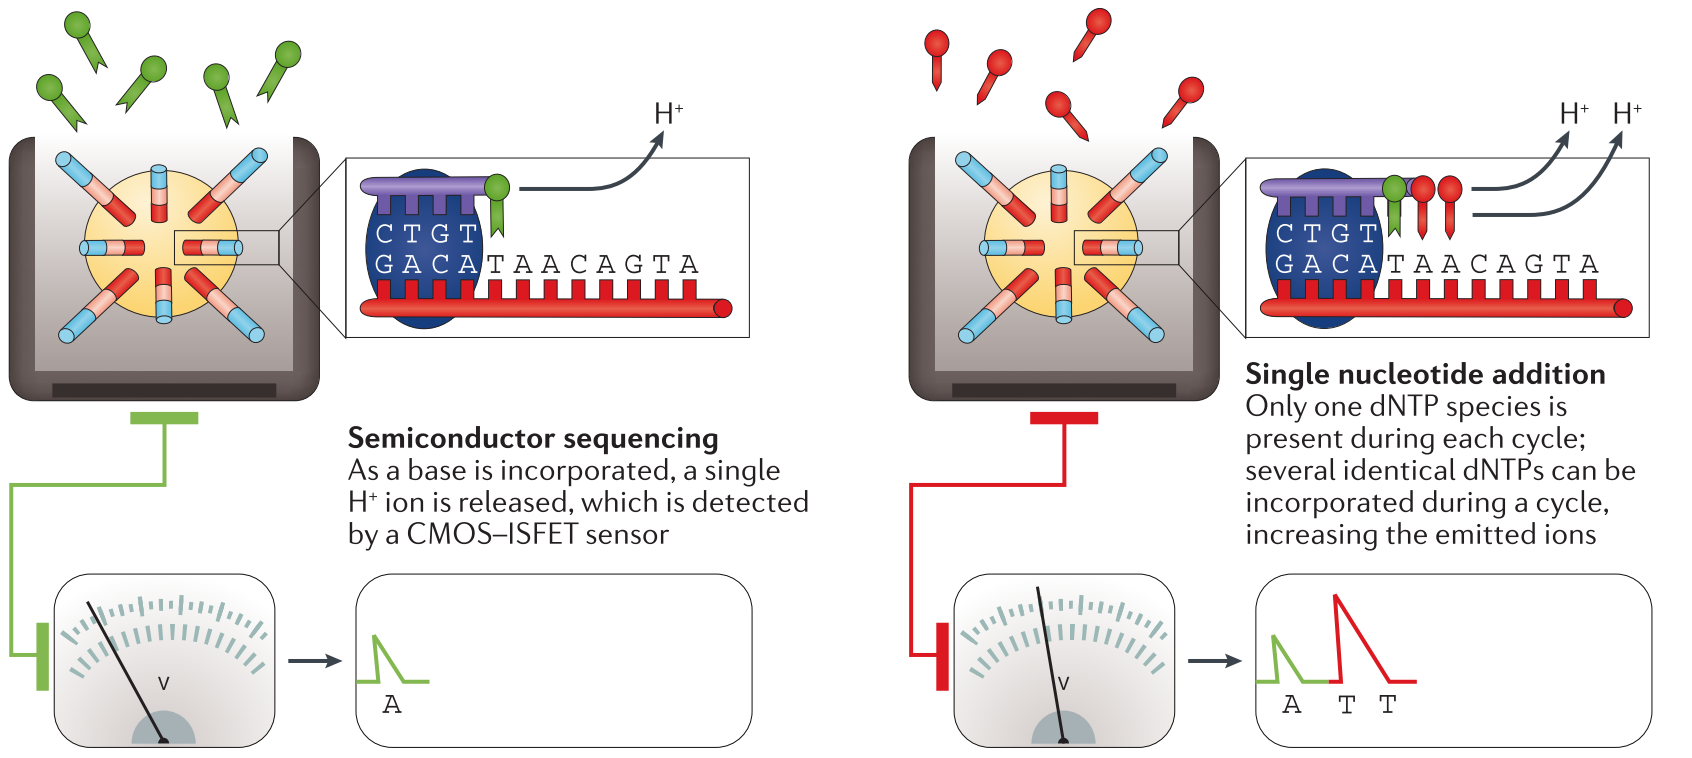
\includegraphics[scale=.26]{figure/SNA_seq_ionTorrent} 

}

\caption[Séquençage SNA tel qu'il est effectué par Ion Torrent]{\textbf{\emph{Séquençage SNA tel qu'il est effectué par
Ion Torrent} d'après {[}\protect\hyperlink{ref-Goodwin2016}{125}{]}} :
\textbf{a} : mise en présence du patron d'ADN à séquencer avec un mix
contenant un seul type de dNTP, si le dNTP est complémentaire au patron,
il se fixe et libère un proton permettant d'identifier la liaison.
\textbf{b} : dans le cas d'homopolymère, autant de protons sont relâchés
que de bases constituant l'homopolymère, le signal émis est donc plus
fort permettant d'identifier le nombre des dNTPs liés.}\label{fig:pictsnaSeq}
\end{figure}










\newpage

\begin{enumerate}
\def\labelenumi{\arabic{enumi}.}
\setcounter{enumi}{1}
\tightlist
\item
  \textbf{Séquençage par ligation} (SBL) (\textbf{Figure :
  }\ref{fig:pictsblSeq}) : Par définition, cette méthode est basée sur
  l'hybridation et la ligation de l'ADN à une sonde liée à un
  fluorophore {[}\protect\hyperlink{ref-Tomkinson2006}{127}{]}. Ce
  processus utilise les caractéristiques de la ligase, une enzyme qui a
  pour fonction de catalyser la liaison de deux brins d'ADN par des
  liaisons phosphodiester. La sonde est constituée d'une de ou deux
  bases connues, on parle alors de \emph{one-base-encoded probes} ou de
  \emph{two-bases-encoded probes} suivies d'une succession de bases
  ``dégénérées'' ou universelles, c'est à dire, de bases capables de
  s'apparier avec n'importe laquelle des quatre bases de l'ADN.
\end{enumerate}

\begin{figure}

{\centering 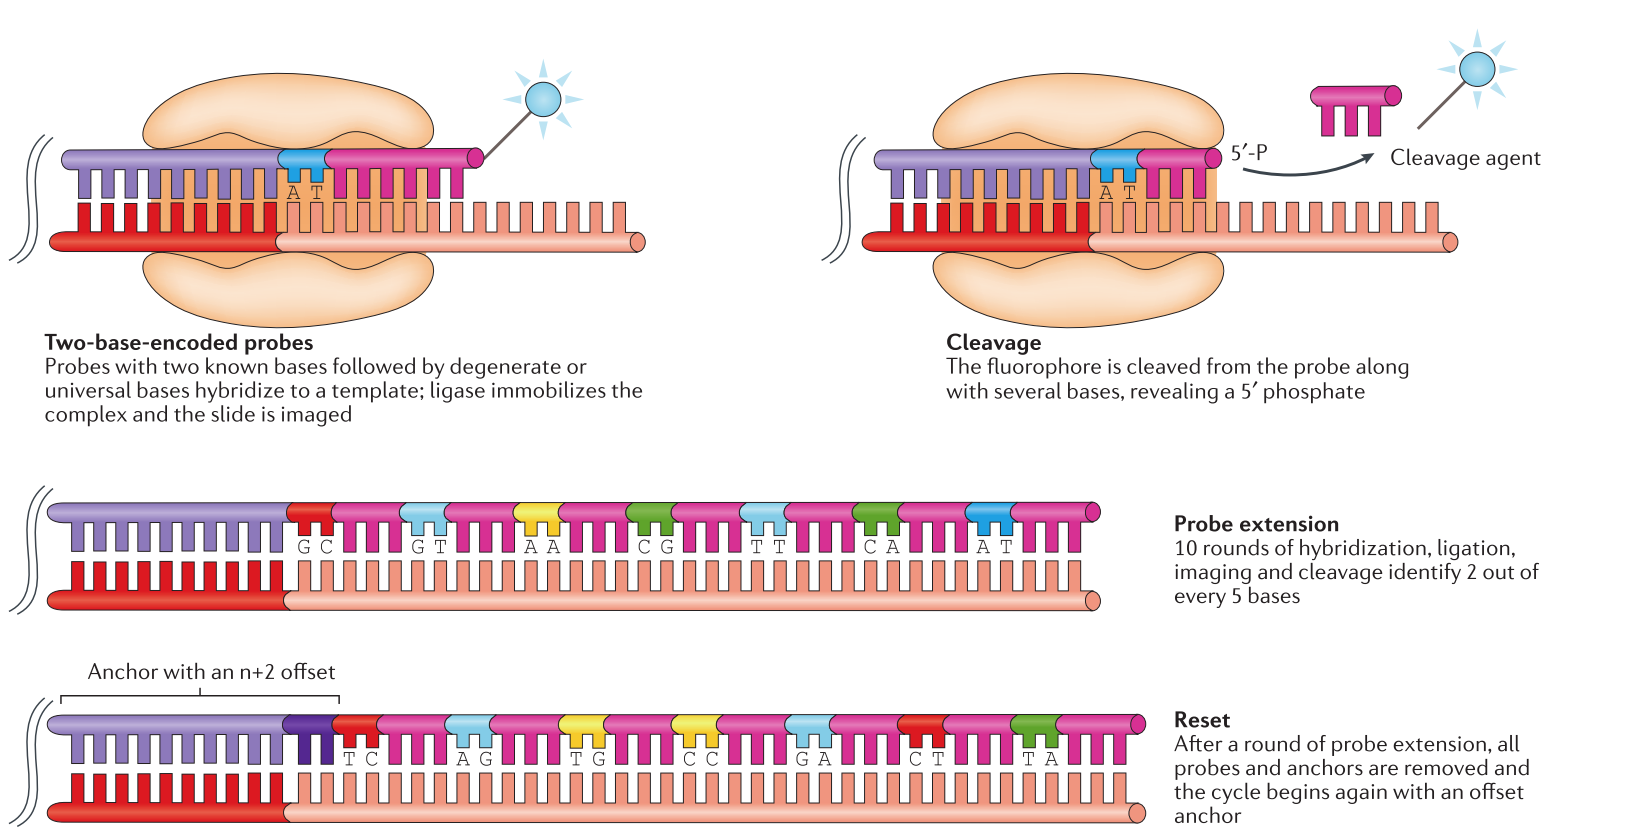
\includegraphics[scale=.26]{figure/SBL_seq_solid} 

}

\caption[Séquençage SBL tel qu'il est effectué par SOLiD]{\textbf{\emph{Séquençage SBL tel qu'il est effectué par
SOLiD} d'après {[}\protect\hyperlink{ref-Goodwin2016}{125}{]}} :
\textbf{a} : dans cette phase d'initialisation, un ensemble de sondes
composées de deux nucléotides connus suivis de bases dégénérées et de
bases universelles est reliée en 5' à un fluorophore. De fait qu'il n'y
ait que quatre fluorophores différents, un même fluorophore est utilisé
pour quatre combinaisons de dinucléotides parmi les seize possibles.
\textbf{b} : après avoir été hybridé grâce à une ligase, aux brin d'ADN
à séquencé, le fluorophore est identifié permettant ainsi de déduire
l'une des quatre combinaisons possibles à ce locus. \textbf{c} : le
fluorophore ainsi qu'une partie des bases non spécifiques sont clivés.
\textbf{d} : les étapes \textbf{b} et \textbf{c} sont ensuite répétées
10 fois permettant à chaque fois d'identifier de réduire la liste des
dinucléotides possibles au locus en question. \textbf{e} : les étapes
\textbf{b}, \textbf{c}, et \textbf{d} sont répétées sur le même brin
avec un décalage d'un nucléotide jusqu'à ce que chaque position ait été
séquencée deux fois. \textbf{f} : en recoupant les informations obtenues
à chaque itération du cycle, la séquence nucléotidique est reconstituée.}\label{fig:pictsblSeq}
\end{figure}




















\newpage  

\section{L'analyse bioinformatique des données de
NGS}\label{lanalyse-bioinformatique-des-donnees-de-ngs}

La stratégie consistant à séquencer en parallèle plusieurs millions de
\emph{reads} courts a engendré de nombreux et nouveaux défis
bioinformatiques dans l'analyse et l'interprétation des données de
séquençage et la recherche de variants dans le génome humain
{[}\protect\hyperlink{ref-Wold2007}{128},
\protect\hyperlink{ref-Yang2009}{129}{]}. Ces techniques ont été
appliquées dans différents contextes, notamment la métagénomique
{[}\protect\hyperlink{ref-Qin2010}{130}{]}, la détection de SNPs
{[}\protect\hyperlink{ref-VanTassell2008}{131}{]} et de variants
structuraux {[}\protect\hyperlink{ref-Alkan2010}{132},
\protect\hyperlink{ref-Medvedev2009}{133}{]} mais également dans des
études portant sur la méthylation de l'ADN
{[}\protect\hyperlink{ref-Taylor2007}{134}{]}, l'analyse de l'expression
des ARNs messagers {[}\protect\hyperlink{ref-Sultan2008}{135}{]}, dans
la génétique du cancer {[}\protect\hyperlink{ref-Guffanti2009}{136}{]}
et la médecine personnalisée
{[}\protect\hyperlink{ref-Auffray2009}{137}{]}. Cependant, pour
l'ensemble de ces applications, la grande quantité de données générées
par chaque analyse pose plusieurs défis informatiques
{[}\protect\hyperlink{ref-Horner2009}{138}{]}. En effet, les progrès
techniques des dernières décennies ont rendu possible le séquençage de
plusieurs millions des \emph{reads} d'ADN en un temps relativement court
et à coût raisonnable. Ainsi, l'émergence du séquençage haut débit et
notamment du WGS et du WES a permis de réunir une quantité jusqu'à
présent inégalée d'informations sur les variations génétiques, et sur
les gènes et leurs fonctions {[}\protect\hyperlink{ref-Mardis2008}{139},
\protect\hyperlink{ref-Bentley2006}{140}{]}. Cependant, de par leur
nature et leur quantité, l'acquisition de ces nouvelles données a
engendré de nouvelles problématiques qui freinent les biologistes dans
leurs recherches.

\subsection{Les données fournies par le
NGS}\label{les-donnees-fournies-par-le-ngs}

\subsubsection{\texorpdfstring{Un \emph{read}, c'est quoi
?}{Un read, c'est quoi ?}}\label{un-read-cest-quoi}

Après la phase d'amplification, chaque clone est analysé, puis la
séquence composant chacun de ce clone est déterminée. La taille de cette
séquence varie en fonction des plateformes de séquençage mais est
généralement comprise entre 40 et 300 pb pour le NGS (\textbf{Figure :
}\ref{fig:pictreadPerRun}). Depuis quelques années, un nouveau type de
\emph{read} est apparu, le \emph{read} \emph{paired-end}. Contrairement
au \emph{reads} classiques (\emph{single-end}), les deux extrémités (les
\emph{ends}) du fragment d'ADN sont désormais séquencées. La distance
approximative séparant les deux extrémités du \emph{read} étant connue,
cela permet aux aligneurs d'utiliser cette information afin d'améliorer
leur précision, notamment dans les zones répétées
{[}\protect\hyperlink{ref-Li2008}{141}{]}. En plus de SNP, ce format
permet de mettre en évidence des variants structuraux
{[}\protect\hyperlink{ref-Korbel2009}{142}{]}.

\newpage

\subsubsection{Le format FASTQ}\label{fastq}

Le format FASTQ (\textbf{Figure : }\ref{fig:pictfastqformat}) est
actuellement le format de données le plus couramment utilisé dans le
cadre du séquençage haut-débit. Sa création est cependant antérieure à
l'émergence du NGS puisqu'il fut inventé à la fin du
XX\textsuperscript{ième} par Jim Mullikin au
\href{https://fr.wikipedia.org/wiki/Wellcome_Trust_Sanger_Institute}{Wellcome
Trust Sanger Institute} alors que le séquençage commençait à prendre de
l'ampleur grâce à des projets tels que le
\href{https://fr.wikipedia.org/wiki/Projet_G\%C3\%A9nome_Humain}{Projet
Génome Humain}. La quantité de données générées par ces programmes a
nécessité une analyse automatisée. C'est ainsi que chaque base séquencée
s'est vu associer un score de qualité appelé \emph{Phred-score}. Chaque
séquence générait ainsi deux fichiers, un fichier FASTA contenant les
séquences et un fichier QUAL contenant les scores \emph{Phred} associés
à chaque base du fichier FASTA
{[}\protect\hyperlink{ref-Cock2009}{143}{]}. Plus tard, afin de n'avoir
à manipuler qu'un seul fichier, les fichiers FASTA et QUAL furent
fusionnés en ce que l'on appelle désormais le fichier FASTQ. Ce format
est aujourd'hui le plus utilisé par les différents séquenceurs. On peut
cependant noter certaines différences dans les formats FASTQ provenant
des différentes plateformes, puisqu'à l'époque, aucune spécification
officielle n'avait été donnée
{[}\protect\hyperlink{ref-Cock2009}{143}{]}.

\begin{figure}

{\centering 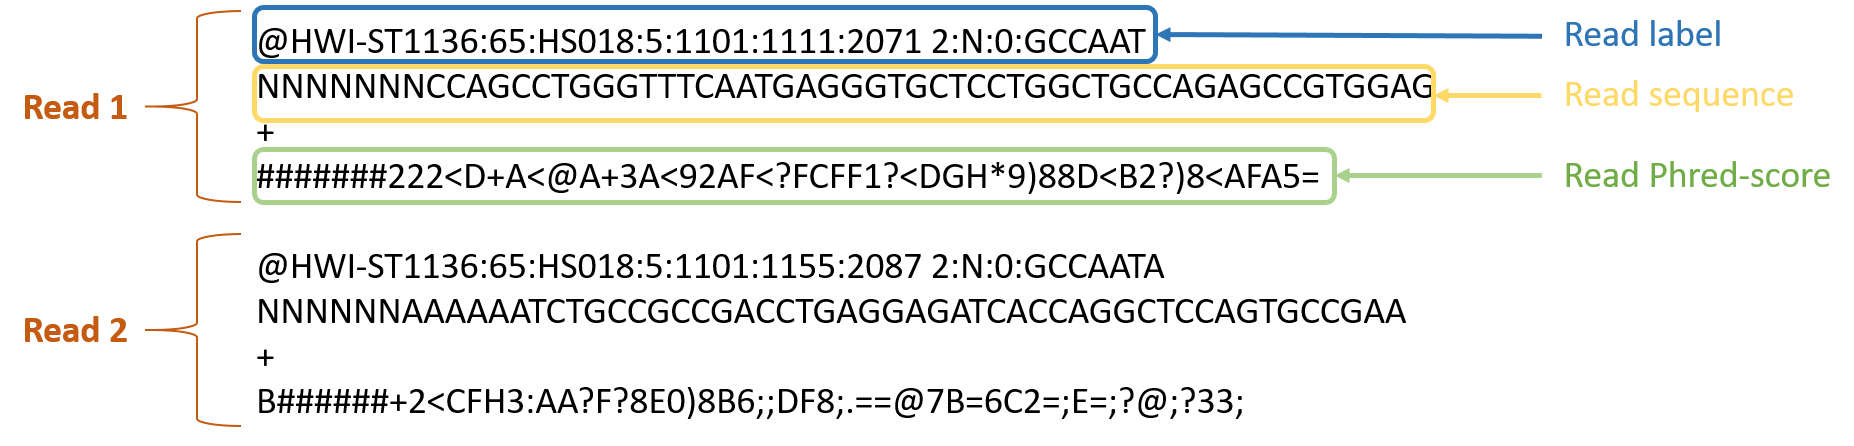
\includegraphics[scale=.34]{figure/fastq} 

}

\caption[Présentation d'un fichier FASTQ]{\textbf{\emph{Présentation d'un fichier FASTQ}} :
Chaque \emph{read} présent au sein d'un fichier FASTQ est composé d'un
label, d'une séquence et d'un score de qualité associé à chaque
nucléotide de la séquence.}\label{fig:pictfastqformat}
\end{figure}






\newpage

\hypertarget{lalignement}{\subsection{L'alignement}\label{lalignement}}

L'alignement constitue la première étape de l'analyse des données de NGS
lorsqu'un génome de référence est disponible. L'objectif de l'alignement
est de déterminer la position correcte de chacun des \emph{reads}
séquencés le long du génome de référence. Cette référence est souvent
construite à partir des données de séquençage de plusieurs donneurs et
ne représente donc pas la séquence d'un individu en particulier mais est
censée représenter la séquence consensus d'une espèce donnée. Par
exemple, la séquence de référence humaine GRCh37 (\emph{Genome Reference
Consortium human build 37}) a été créée à partir de treize volontaires
anonymes New-Yorkais. Dès lors, cette référence servira de patron aux
aligneurs afin qu'ils replacent correctement les différents \emph{reads}
des individus séquencés. Cette étape peut être comparée à la
reconstruction d'un puzzle dans lequel les \emph{reads} seraient les
pièces et le génome de référence le modèle (\textbf{Figure :
}\ref{fig:picdnamapping}). Elle constitue probablement l'étape la plus
importante de l'analyse des données issues du séquençage haut débit
{[}\protect\hyperlink{ref-Flicek2009}{144}{]} car elle est la base sur
laquelle repose l'ensemble des étapes effectuées en aval, notamment
l'appel des variants {[}\protect\hyperlink{ref-Nielsen2011}{145}{]}.
Cependant, l'étape d'alignement est sujette à de nombreuses erreurs dont
certaines proviennent directement des erreurs survenues lors de l'étape
de séquençage. D'autres, sont dues aux caractéristiques des régions
séquencées comme par exemple les séquences répétées
{[}\protect\hyperlink{ref-Langmead2012}{146}{]} qui pourront entraîner
l'alignement d'un même \emph{read} à plusieurs régions du génome
{[}\protect\hyperlink{ref-Treangen2013}{147}{]}. De nombreux aligneurs
ont émergé afin de répondre au mieux à cette problématique tel que
Bowtie {[}\protect\hyperlink{ref-Langmead2009}{148}{]}, Bowtie2
{[}\protect\hyperlink{ref-Langmead2012}{146}{]}, BWA, NovoAlign, MAGIC
{[}\protect\hyperlink{ref-Su2014}{149}{]}. De nombreuses études ont
cependant montré de grandes différences entre ces aligneurs, au niveau
du temps de calcul, de leur coût en mémoire et de leur taux d'erreur
{[}\protect\hyperlink{ref-Ruffalo2011}{150}--\protect\hyperlink{ref-Bao2011}{152}{]}.

\newpage

\begin{figure}

{\centering \includegraphics[scale=0.35]{figure/dna_mapping} 

}

\caption[Représentation schématique de l'alignement de reads paired-end]{\textbf{\emph{Représentation schématique de
l'alignement de reads paired-end}} : \textbf{A} : représentation du
génome de référence ainsi que de \emph{reads paired-end} avant l'étape
d'alignement. Les \emph{reads paired-end} sont composés d'une extrémité
\emph{forward} (en vert) complémentaire du brin sens du génome de
référence et d'une extrémité réverse (en jaune), complémentaire du brin
anti-sens du génome de référence. Chacune de ces extrémités est séparée
par un insert de taille connue mais de séquence inconnu. \textbf{B} :
après l'étape d'alignement, chaque \emph{read} est repositionné sur la
région du génome avec laquelle il présente la plus grande homologie de
séquence. Le nombre de \emph{reads} différents recouvrant une même
position du génome de référence est appelé couverture.}\label{fig:picdnamapping}
\end{figure}














\newpage

\subsection{L'appel des variants}\label{varcall}

L'appel des variants, ou \emph{variant calling}, fait référence à
l'ensemble des méthodes permettant d'identifier des SNVs ou des indels à
partir des résultats de l'alignement. Cette étape est souvent
différenciée de l'alignement, cependant, les résultats de l'appel étant
extrêmement dépendants de l'alignement, il est conseillé d'effectuer son
appel en tenant compte de l'aligneur choisi
{[}\protect\hyperlink{ref-Nielsen2011}{145},
\protect\hyperlink{ref-DePristo2011}{153},
\protect\hyperlink{ref-Lunter2011}{154}{]}. On appellera variant toute
différence de séquence observée entre un individu et la séquence de
référence utilisée. Pour reprendre la comparaison avec la construction
d'un puzzle, cette étape consiste à détecter quelles sont les pièces qui
présentent des différences avec le modèle.

\begin{figure}

{\centering \includegraphics[scale=0.33]{figure/var_call_exemple} 

}

\caption[Illustration schématique du processus d'appel des variants]{\textbf{\emph{Illustration schématique du
processus d'appel des variants}} : Pour chaque position couverte, le
pourcentage de \emph{read} portant un allèle variant est analysé.
Lorsque l'on est proche des 100\% l'appel est homozygote pour le
variant, lorsque l'on est proche des 50\% l'appel des hétérozygote.
Lorsqu'à une position donnée, peu de \emph{reads} portent un variant, la
cause est souvent une erreur de séquençage.}\label{fig:picvarcallprocess}
\end{figure}









De nombreux logiciels d'appels des variants, ou \emph{caller}, basés sur
des algorithmes différents ont émergé ces dernières années pour répondre
à cette problématique. Parmi les plus connus on note SAMtools
{[}\protect\hyperlink{ref-Li2009}{155}{]}, Genome Analysis Tool Kit -
HaplotypeCaller (GATK-HC)
{[}\protect\hyperlink{ref-McKenna2010}{156}{]}, Freebayes, SOAPindel et
TVC. Les quatre premiers cités, peuvent être utilisés pour analyser des
données provenant de tout type de plateforme de séquençage contrairement
à TVC qui a été développé spécifiquement pour les données provenant de
Ion Proton. Les données issues de NGS peuvent présenter un taux d'erreur
important. Ce taux d'erreur est multifactoriel et inclut notamment les
erreurs de l'alignement. L'un des éléments clef à prendre en compte pour
pouvoir effectuer un appel de qualité est la couverture de la position
appelée {[}\protect\hyperlink{ref-Sims2014}{120}{]}. Cependant, malgré
la prise en compte de cet élément, l'appel de variants reste un
processus difficile souvent lié à plusieurs erreurs. Plusieurs de ces
erreurs sont même directement liées à la plateforme de séquençage
utilisée en amont, et les différents logiciels ne présentent pas les
mêmes performances en fonction de ces différentes plateformes
{[}\protect\hyperlink{ref-Hwang2015}{157}{]}. C'est pourquoi, il
convient d'adapter le logiciel d'appel en fonction de la plateforme de
séquençage utilisée préalablement. Les erreurs d'appel sont généralement
classées en trois catégories et certains aligneurs auront tendance à
être plus sujets à l'un de ces types d'erreur qu'à l'autre
(\textbf{Figure : }\ref{fig:pictsnperror}) :

\begin{enumerate}
\def\labelenumi{\arabic{enumi}.}
\item
  Oubli de l'allèle de référence (\textbf{IR}, \emph{ignore the
  reference allele}) : représente un variant appelé homozygote
  correspondant en réalité à un variant hétérozygote composé de l'allèle
  de référence et d'un allèle variant.
\item
  Ajout de l'allèle de référence (\textbf{AR}, \emph{adding the
  reference allele}) : représente un variant appelé hétérozygote composé
  de l'allèle de référence et d'un allèle variant correspondant en
  réalité à un variant homozygote composé de deux allèles variants.
\item
  Autres : incluent l'ensemble des autres types d'appel erronés
  indépendamment de l'allèle de référence.
\end{enumerate}

\begin{figure}

{\centering 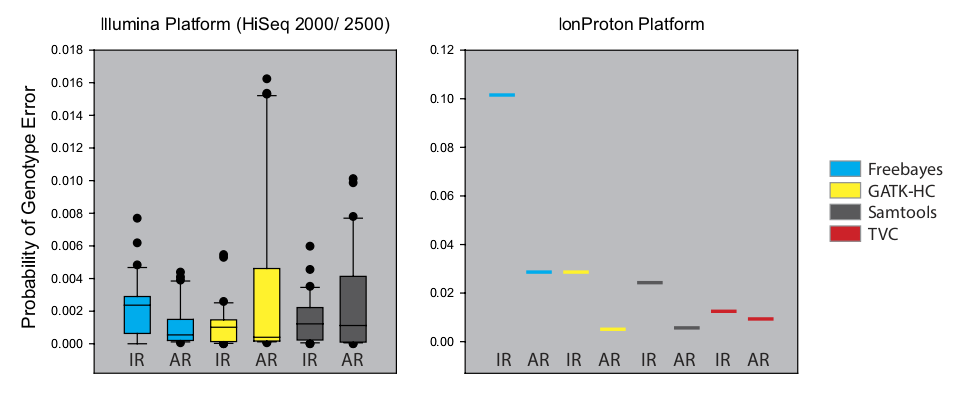
\includegraphics[scale=.37]{figure/snp_error_type} 

}

\caption[Représentation des erreurs d'appel de type IR et AR en fonction de la plateforme de séquençage et du logiciel d'appel]{\textbf{\emph{Représentation des erreurs d'appel de
type IR et AR en fonction de la plateforme de séquençage et du logiciel
d'appel} d'après {[}\protect\hyperlink{ref-Hwang2015}{157}{]}} : Pour la
plateforme Illumina, on peut voir que Freebayes favorise les appels
variant-homozygote tandis que GATK-HC et Samtools favorisent les appels
hétérozygotes. Pour la plateforme Ion Proton, les quatre logiciels
entraînent des erreurs de type IR}\label{fig:pictsnperror}
\end{figure}









De même que pour l'aligneur, le choix du logiciel d'appel est crucial
car il existe de nombreuses différences dans les variants appelés par
différents logiciels se basant sur les mêmes données brutes
{[}\protect\hyperlink{ref-Baes2014}{158}--\protect\hyperlink{ref-Rosenfeld2012}{160}{]}.
En effet, en 2013, une étude comparant les résultats de 5 \emph{callers}
montraient que seulement 57,4\% des variants étaient appelés par les 5
\emph{callers} et que 80,7\% des variants étaient appelés par au moins 3
d'entre eux. Ce taux chutait drastiquement pour les indels puisque la
concordance était cette fois seulement de 26,8\% pour les indels non
retrouvés par les 3 \emph{callers}
{[}\protect\hyperlink{ref-ORawe2013}{159}{]}. Ces résultats sont
cependant à pondérer avec une étude de 2015 comparant 4 \emph{callers}
et montrant que 91,7\% des SNVs séquencés sur une plateforme Illumina
étaient appelés par 3 \emph{callers}, cependant, pour les variants
séquencés sur Ion Proton, seulement 27,3\% des variants étaient appelés
par au moins 3 \emph{callers} et 57,4\% des variants n'étaient appelés
que par un seul des \emph{callers}
{[}\protect\hyperlink{ref-Hwang2015}{157}{]}.

\newpage

\subsection{L'annotation des variants}\label{lannotation-des-variants}

Traditionnellement, les scientifiques et les laboratoires dans lesquels
ils travaillaient développaient leur expertise dans un nombre de
pathologies et de gènes associés limité. L'émergence du NGS est en train
de remettre en cause cette pratique car la totalité de l'exome ou du
génome peut permettre de couvrir tous les gènes en une seule et même
analyse. De nombreux praticiens maintiennent cependant une
spécialisation pour certains groupes de pathologies qui est précieuse
pour l'analyse des données et l'obtention d'un diagnostic. En effet il
est courant de retrouver entre 20.000 et 25.000 variants différents par
exome {[}\protect\hyperlink{ref-Gonzaga-Jauregui2012}{161}{]}. Afin de
pouvoir lier un variant à une pathologie, il est indispensable d'annoter
cet ensemble de variants, c'est à dire d'associer à ces variants
l'ensemble des informations qui les caractérisent afin de pouvoir les
replacer dans leur contexte biologique. Ces informations serviront
ensuite d'indicateur afin de filtrer ou de prioriser un variant. Cette
dernière étape de l'analyse est, elle aussi, cruciale puisqu'elle permet
de réduire le nombre de variants à considérer. On peut généralement
distinguer deux niveaux d'annotations d'un variant (\textbf{Figure :}
\ref{fig:pictannot}) :

\begin{enumerate}
\def\labelenumi{\arabic{enumi}.}
\tightlist
\item
  \textbf{Au niveau du variant} : Ce niveau d'annotation regroupe
  l'ensemble des informations \textbf{spécifiques} à un variant

  \begin{enumerate}
  \def\labelenumii{\alph{enumii}.}
  \item
    \textbf{Informations issues des résultats du séquençage} : la
    couverture du variant ainsi que la qualité qui lui est associée
    peuvent permettre de considérer un variant comme étant fiable ou
    non. Le génotype associé à ce variant est également une information
    importante.
  \item
    \textbf{La fréquence du variant dans la population générale} :
    l'émergence du séquençage haut-débit a permis de gros consortiums
    tels que ESP6500 (\href{http://evs.gs.washington.edu/EVS/}{Exome
    Variant Server, NHLBI GO Exome Sequencing Project (ESP), Seattle,
    WA}), 1KG
    {[}\protect\hyperlink{ref-1000GenomesProjectConsortium2015}{162}{]}.
    Ces consortiums ont pu mettre à disposition du public des données de
    séquençage exomique de 6503 individus pour ESP et de 2504 pour la
    phase 3 du 1000Genomes. On peut également noter l'\emph{Exome
    Aggregate Consortium} (ExAC)
    {[}\protect\hyperlink{ref-Lek2016}{163}{]} qui n'a effectué aucun
    séquençage mais qui a regroupé les données de plusieurs gros jeux
    (notamment 1000Genome et ESP) afin de leur appliquer la même analyse
    bioinformatique harmonisant ainsi les données provenant de 60.706
    individus non apparentés. Cette masse d'information permet de se
    faire une idée de la fréquence d'un variant dans la population
    générale et même au sein de sous-populations humaines. On considère
    qu'un variant fréquent ne peut pas être délétère, sinon il aurait
    été contre-sélectionné au cours de l'évolution.
  \item
    \textbf{Son impact sur le transcrit} : Dans la plupart des analyses
    phénotype-génotype, les chercheurs se limitent aux variants
    chevauchant des transcrits codants pour une protéine. Il est donc
    important de savoir l'impact d'un variant sur ce transcrit, c'est à
    dire si le variant va causer une mutation synonyme, un faux-sens ou
    une mutation tronquante. Des logiciels tels que \emph{Variant Effect
    Predictor} (VEP) {[}\protect\hyperlink{ref-McLaren2016}{164}{]},
    SnpEff {[}\protect\hyperlink{ref-Cingolani2012}{165}{]} ou encore
    ANNOVAR {[}\protect\hyperlink{ref-Wang2010}{166}{]} vont prédire
    l'impact qu'aura un variant sur les différents transcrits qu'il
    chevauche. D'autres logiciels tel que SIFT
    {[}\protect\hyperlink{ref-Kumar2009}{167}{]}, PROVEAN
    {[}\protect\hyperlink{ref-Choi2012}{168}{]}, Polyphen2, ou encore
    CADD vont, eux, chercher à prédire la pathogénicité de ce variant,
    c'est à dire la probabilité que ce variant soit délétère pour la
    fonction de la protéine. Bien que cette information soit importante,
    elle est à pondérer, étant donné le peu de concordance qu'il existe
    entre les prédictions de ces différents logiciels (\textbf{Figure :}
    \ref{fig:pictvennpred}).
  \end{enumerate}
\end{enumerate}

\begin{figure}

{\centering 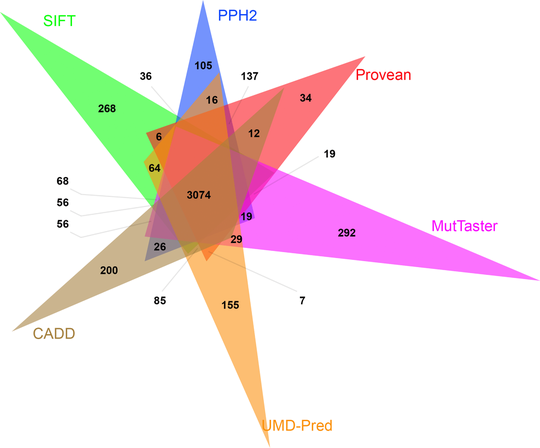
\includegraphics[scale=.7]{figure/venn_Diag_patho_pred} 

}

\caption[Diagramme de Venn des prédictions de pathogénicité de variants de six logiciels]{\textbf{\emph{Diagramme de Venn des prédictions de
pathogénicité de variants de six logiciels} d'après
{[}\protect\hyperlink{ref-Salgado2016}{169}{]}} : Les six logiciels
utilisés sont : CADD {[}\protect\hyperlink{ref-Kircher2014}{170}{]}
(marron), SIFT {[}\protect\hyperlink{ref-Kumar2009}{167}{]} (vert),
PolyPhen2 {[}\protect\hyperlink{ref-Adzhubei2010}{171}{]} (bleu),
Provean {[}\protect\hyperlink{ref-Choi2012}{168}{]} (rouge)
MutationTaster {[}\protect\hyperlink{ref-Schwarz2010}{172}{]} (violet)
et UMD-Predictor {[}\protect\hyperlink{ref-Salgado2016a}{173}{]}
(orange).}\label{fig:pictvennpred}
\end{figure}












\newpage

\begin{enumerate}
\def\labelenumi{\arabic{enumi}.}
\setcounter{enumi}{1}
\tightlist
\item
  \textbf{Au niveau du gène (ou transcrit)} : L'annotation au niveau du
  gène consiste à récupérer l'ensemble des informations disponibles non
  plus sur le variant uniquement mais sur le ou les gènes qu'il impacte.
  Ce ``dézoom'' permet d'ajouter des informations complémentaires
  particulièrement utiles notamment lorsque peu d'informations sont
  disponibles sur le variant lui-même. En pratique, la plupart des
  variants connus pour impliquer une pathologie sont des variants
  privés, c'est à dire spécifiques à une famille ou à un individu,
  limitant ainsi la quantité d'information disponible sur ce variant.
  Élargir l'annotation au niveau des gènes impactés par des variants
  permet d'augmenter considérablement la quantité d'information
  disponible et permet donc d'améliorer la capacité des algorithmes à
  filtrer et / ou prioriser les variants rendant donc les analyses plus
  efficaces. On peut relever certains logiciels tel que le \emph{Protein
  ANalysis THrough Evolutionary Relationships} (PANTHER)
  {[}\protect\hyperlink{ref-Mi2017}{174}{]} qui permettent par exemple
  de classer une liste de gènes en fonction de leurs fonctions
  moléculaires, des processus biologiques et des voies de signalisation
  dans lesquelles ils sont impliqués. On peut également noter \emph{the
  Human Phenotype Ontology project} (HPO)
  {[}\protect\hyperlink{ref-Kohler2014}{175}{]} qui fournit un
  vocabulaire standardisé pour les anomalies phénotypiques observées
  dans les pathologies humaines et une liste de gènes connus pour être
  associés à ces phénotypes. Plus récemment, on a pu voir émerger des
  ``scores mutationnels'' tel que RVIS
  {[}\protect\hyperlink{ref-Petrovski2013}{176}{]} ou encore le pLI
  {[}\protect\hyperlink{ref-Lek2016}{163}{]}. En se basant sur les bases
  de données telle que ESP ou encore ExAC, ces scores permettent de
  classer les gènes en fonction de leur tolérance (ou intolérance) aux
  variations avec l'idée sous-jacente que ``les gènes impliqués dans des
  pathologies à transmission mendéliennes'' devraient être moins
  tolérants aux variations que les autres.
\end{enumerate}

\begin{figure}

{\centering \includegraphics[scale=.25]{figure/annotation_process} 

}

\caption[Représentation simplifié du processus d'annotation]{\textbf{\emph{Représentation simplifié du processus
d'annotation}} : On peut observer deux niveaux d'annotation, le premier
est l'annotation des variants consistant à ajouter un maximum
d'information sur un variant spécifique (sa fréquence, son
impact\ldots{}). La deuxième est au niveau du gène, consistant à
récupérer pour les gènes impactés par les variants l'ensemble des
informations disponibles tel que les processus biologiques dans lesquels
il est impliqué, ou encore son expression tissulaire.}\label{fig:pictannot}
\end{figure}










\newpage

\subsection{Le filtrage des variants}\label{le-filtrage-des-variants}

L'étape de filtrage a pour principal objectif de restreindre le nombre
de variants obtenu à l'issus de l'appel afin que ceux-ci puissent être
analysés par un être humain. Pour cela il utilise l'ensemble des
information obtenues lors de l'étape d'annotation afin de filtrer les
variants ayant le moins de risque d'être responsables du phénotype.
Communément, les variant ayant une forte fréquence dans les bases de
données ExAC, ESP6500 ou encore 1KG sont filtrés avec l'idée
sous-jacente que des variants observés fréquemment dans la population ne
peuvent être responsables de phénotypes sévères.

Comme nous l'avons vu, le développement d'outils permettant l'analyse et
le filtrage des données NGS est extrêmement important puisqu'il permet
aux biologistes de faire face à la masse de données générée par le
séquençage haut-débit l'aidant ainsi dans ses prises de décisions. Il
est à noter que la plupart de ces données filtrées sont extrêmement
dépendantes du jeu de transcrits utilisés. Les prédictions seront donc
différentes si l'on se base sur les transcrits RefSeq, Ensembl ou UCSC
{[}\protect\hyperlink{ref-McCarthy2014}{177}{]} bien que les transcrits
du \emph{Consensus Coding Sequence project} (CCDS) soient bien
représentés par ces trois listes
{[}\protect\hyperlink{ref-Pruitt2009}{179}{]}. De même, pour une même
liste de gène, de nombreuses différences seront observées en fonction du
ou des logiciels de prédiction utilisés
{[}\protect\hyperlink{ref-Salgado2016}{169},
\protect\hyperlink{ref-McCarthy2014}{177}{]}.

\begin{figure}

{\centering \includegraphics[scale=.25]{figure/filtering_process} 

}

\caption[Représentation simplifié du processus de filtrage des variants]{\textbf{\emph{Représentation simplifié du processus de
filtrage des variants}} : L'ensemble des annotations ajoutées lors de
l'étape précédente servent alors de support pour filtrer (ou non) les
variants. Il est par exemple commun de filtrer les variants ayant une
forte fréquence dans la population générale ou encore ceux ayant un
impact faible sur la protéine. De même dans le cas d'étude sur des
pathologies ayant un mode de transmission récessif, les variants
hétérozygotes pourront être également filtrés.}\label{fig:pictfilter}
\end{figure}










\newpage

\subsection{Conclusion NGS}\label{conclusion-ngs}

En moins de 10 ans, les technologies NGS sont passées du séquençage de
panels de gènes (environ 100 Mb pour le Roche GS FLX system) au
séquençage de génomes entiers (environs 1500 GB pour l'Illumina Hiseq
4000) et d'une utilisation exclusive à la recherche à l'analyse en
routine dans un cadre de diagnostics cliniques. Le nombre croissant
d'études utilisant le WGS ou le WES démontre le pouvoir de ces approches
dans des analyses phénotype-génotype impliquant des pathologies à
transmission mendélienne. De plus, la diminution constante des coûts par
génomes / exomes séquencés laisse supposer que ces technologies
deviendront d'ici peut le fer de lance de la génétique clinique moderne.
Cependant, la quantité de données produites crée de nouvelles
problématiques pour les généticiens qui se retrouvent désormais face au
``déluge de données génétiques''
{[}\protect\hyperlink{ref-Schatz2013}{180}{]}. Le succès d'une étude
n'étant plus lié aux capacités de séquençage mais aux compétences dans
l'analyse et l'interprétation des données produites à chaque étape
(\textbf{Figure :} \ref{fig:pictrecapngssteps}). Bien que de nombreux
efforts soient faits pour palier la contrainte instaurée par les
\emph{reads} courts dans le cadre d'analyse génomique, les solutions
informatiques et bioinformatiques proposées jusqu'à présent restent en
dessous des besoins créés par NGS
{[}\protect\hyperlink{ref-McPherson2009}{181}{]}. Cette masse de données
produite, à l'origine du succès du séquençage haut-débit dans le domaine
de la génomique et de la post-génomique, se trouve désormais être un
frein à la compréhension et à l'interprétation des réseaux de gènes et
leurs implications dans des pathologies. La limitation de cette
technologie n'est donc plus le séquençage d'un, de plusieurs, ou de
l'ensemble des gènes, mais plutôt l'analyse et l'interprétation des
données générées. Le processus allant de l'extraction de l'ADN à
l'identification d'un variant responsable d'une pathologie comprend de
nombreuses étapes apportant avec elles leurs lots d'erreurs. Bien que
dans chacune de ces phases, de nombreux acteurs soient en concurrence et
cherchent à atteindre une solution idéale, celle-ci n'a toujours pas été
trouvée et la prolifération des logiciels et algorithmes d'analyses,
bien que nécessaire, peut également parfois augmenter la confusion.

Malgré les dizaines de milliers d'exomes et de génomes ayant été jusqu'à
présent étudiés, notre compréhension des mécanismes moléculaires qui
sous-tendent la variété génomique humaine reste limitée, et ce
particulièrement dans le contexte de l'analyse de pathologies
génétiques. En effet, à l'heure actuelle, plus de 3700 pathologies à
transmission mendélienne ont été caractérisées mais un nombre similaire
a toujours une cause inconnue
{[}\protect\hyperlink{ref-Amberger2011}{182}{]}. L'élucidation de ces
mystères passera probablement par une harmonisation des méthodes de
production des données ainsi que par l'amélioration des techniques
d'analyses.

\newpage 

\begin{figure}

{\centering \includegraphics[scale=.3]{figure/bioinformatic_steps} 

}

\caption[Récapitulatif des différentes étapes du séquençage NGS dans le cadre d'une étude phénotype-génotype]{\textbf{\emph{Récapitulatif des différentes
étapes du séquençage NGS dans le cadre d'une étude phénotype-génotype}}
: L'ADN est d'abord extrait, puis fragmenté. Les fragments sont liés à
des adaptateurs puis amplifiés. Ces amplifiats sont alors isolés et
soumis à une amplification clonale (schéma de l'amplification clonale
est adapté d'après {[}\protect\hyperlink{ref-Goodwin2016}{125}{]}).
Chacun des clones est ensuite séquencé. Les \emph{reads} générés à
l'issu du séquençage sont stockés dans des fichiers FASTQ qui serviront
de base pour l'étape d'alignement à la suite de laquelle, les variants
et leur génotype seront appelés puis annotés. Ces annotations serviront
ensuite pour filtrer les variants jugés non pertinent dans le cadre de
l'étude, les variants / gènes restant seront ensuite prioriser de sorte
à identifier le/les variant(s) responsable(s) du phénotype.}\label{fig:pictrecapngssteps}
\end{figure}















\chapter{Mise en place d'une stratégie pour l'analyse des données
exomiques -- application en recherche
clinique}\label{mise-en-place-dune-strategie-pour-lanalyse-des-donnees-exomiques-application-en-recherche-clinique}

\section{Méthode : Description du
pipeline}\label{methode-description-du-pipeline}

\subsection{\texorpdfstring{L'alignement des
\emph{reads}}{L'alignement des reads}}\label{lalignement-des-reads}

\subsection{L'appel des variants}\label{lappel-des-variants}

\subsection{L'annotation}\label{lannotation}

\subsection{Le filtrage des variants}\label{le-filtrage-des-variants-1}

\section{Résultats 1 : Analyse de 3 phénotypes par des cas
familiaux}\label{resultats-1-analyse-de-3-phenotypes-par-des-cas-familiaux}

\subsection{Résultats des différentes étapes de
l'analyse}\label{resultats-des-differentes-etapes-de-lanalyse}

\subsubsection{Résultat de l'alignement}\label{resultat-de-lalignement}

\subsubsection{L'appel des variants}\label{lappel-des-variants-1}

\subsubsection{L'annotation des
variants}\label{lannotation-des-variants-1}

\subsubsection{Le filtrage des
variants}\label{le-filtrage-des-variants-2}

\subsection{Article n°1}\label{article-n1}

\subsubsection{Contexte et objectifs}\label{contexte-et-objectifs}

\subsubsection{Principaux résultats}\label{principaux-resultats}

\subsection{Article n°2}\label{article-n2}

\subsubsection{Contexte et objectifs}\label{contexte-et-objectifs-1}

\subsubsection{Principaux résultats}\label{principaux-resultats-1}

\subsection{Article n°3}\label{article-n3}

\subsubsection{Contexte et objectifs}\label{contexte-et-objectifs-2}

\subsubsection{Principaux résultats}\label{principaux-resultats-2}

\section{Résultats 2 : Étude d'une cohorte de femmes
infertiles}\label{resultats-2-etude-dune-cohorte-de-femmes-infertiles}

\subsection{Article n°4}\label{article-n4}

\subsubsection{Contexte et objectifs}\label{contexte-et-objectifs-3}

\subsubsection{Principaux résultats}\label{principaux-resultats-3}

\section{Résultats 3 : Étude d'une large cohorte de patients
MMAF}\label{resultats-3-etude-dune-large-cohorte-de-patients-mmaf}

\subsection{Article n°5}\label{article-n5}

\subsubsection{Contexte et objectifs}\label{contexte-et-objectifs-4}

\subsubsection{Principaux résultats}\label{principaux-resultats-4}

\hypertarget{globo}{\chapter{Investigation génétique et physiologique de
la globozoospermie}\label{globo}}

\section{Introduction sur la
globozoospermie}\label{introduction-sur-la-globozoospermie}

\section{\texorpdfstring{Résultats 1 : Les mécanismes mutationnels
entraînant la délétion au locus de \emph{DPY19L2} chez
l'humain}{Résultats 1 : Les mécanismes mutationnels entraînant la délétion au locus de DPY19L2 chez l'humain}}\label{mecamut}

\subsection{Article n°6:}\label{article-n6}

\subsubsection{Contexte et objectifs}\label{contexte-et-objectifs-5}

\subsubsection{Principaux résultats}\label{principaux-resultats-5}

\section{Résultat 2 : La transcriptomique}\label{transcriptome}

\subsection{Article n°7:}\label{article-n7}

\subsubsection{Contexte et objectifs}\label{contexte-et-objectifs-6}

\subsubsection{Principaux résultats :}\label{principaux-resultats-6}

\chapter{This chunk ensures that the thesisdown package
is}\label{this-chunk-ensures-that-the-thesisdown-package-is}

\chapter{Article annexe}\label{dnah12014}

\chapter*{References}\label{references}
\addcontentsline{toc}{chapter}{References}

\hypertarget{refs}{}
\hypertarget{ref-Tosti2016}{}
1. E. Tosti and Y. Ménézo: ``Gamete activation: basic knowledge and
clinical applications.'' \emph{Human Reproduction Update}. vol. 22, no.
4, pp. 420--439, 2016.

\hypertarget{ref-Stricker}{}
2. S.A. Stricker: ``Comparative Biology of Calcium Signaling during
Fertilization and Egg Activation in Animals.'' \emph{Developmental
Biology}. vol. 211, no. 2, pp. 157--176, 1999.

\hypertarget{ref-Miyazaki1993}{}
3. S. Miyazaki, H. Shirakawa, K. Nakada, and Y. Honda: ``Essential role
of the inositol 1,4,5-trisphosphate receptor/Ca2+ release channel in
Ca2+ waves and Ca2+ oscillations at fertilization of mammalian eggs.''
\url{http://www.sciencedirect.com/science/article/pii/S0012160683711681},
(1993).

\hypertarget{ref-Swann1990}{}
4. K. Swann: ``A cytosolic sperm factor stimulates repetitive calcium
increases and mimics fertilization in hamster eggs.''
\emph{Development}. vol. 110, no. 4, 1990.

\hypertarget{ref-Sun1992}{}
5. F.Z. Sun, J. Hoyland, X. Huang, W. Mason, R.M. Moor, and P. Rossi:
``A comparison of intracellular changes in porcine eggs after
fertilization and electroactivation.'' \emph{Development (Cambridge,
England)}. vol. 115, no. 4, pp. 947--56, 1992.

\hypertarget{ref-Lawrence1997}{}
6. Y. Lawrence, M. Whitaker, and K. Swann: ``Sperm-egg fusion is the
prelude to the initial Ca2+ increase at fertilization in the mouse.''
\emph{Development (Cambridge, England)}. vol. 124, no. 1, pp. 233--41,
1997.

\hypertarget{ref-Wu1997}{}
7. H. Wu, C.L. He, and R.A. Fissore: ``Injection of a porcine sperm
factor triggers calcium oscillations in mouse oocytes and bovine eggs.''
\emph{Molecular Reproduction and Development}. vol. 46, no. 2, pp.
176--189, 1997.

\hypertarget{ref-Wu1998}{}
8. H. Wu, C.-L. He, B. Jehn, S.J. Black, and R.A. Fissore: ``Partial
Characterization of the Calcium-Releasing Activity of Porcine Sperm
Cytosolic Extracts.'' \emph{Developmental Biology}. vol. 203, no. 2, pp.
369--381, 1998.

\hypertarget{ref-Stricker1997}{}
9. S.A. Stricker: ``Intracellular Injections of a Soluble Sperm Factor
Trigger Calcium Oscillations and Meiotic Maturation in Unfertilized
Oocytes of a Marine Worm.'' \emph{Developmental Biology}. vol. 186, no.
2, pp. 185--201, 1997.

\hypertarget{ref-Tang2000}{}
10. T.S. Tang, J.B. Dong, X.Y. Huang, and F.Z. Sun: ``Ca(2+)
oscillations induced by a cytosolic sperm protein factor are mediated by
a maternal machinery that functions only once in mammalian eggs.''
\emph{Development (Cambridge, England)}. vol. 127, no. 5, pp. 1141--50,
2000.

\hypertarget{ref-Saunders2002}{}
11. C.M. Saunders, M.G. Larman, J. Parrington, L.J. Cox, J. Royse, L.M.
Blayney, K. Swann, and F.A. Lai: ``PLC zeta: a sperm-specific trigger of
Ca(2+) oscillations in eggs and embryo development.'' \emph{Development
(Cambridge, England)}. vol. 129, no. 15, pp. 3533--44, 2002.

\hypertarget{ref-Clift2013}{}
12. D. Clift and M. Schuh: ``Restarting life: fertilization and the
transition from meiosis to mitosis.'' \emph{Nature Reviews Molecular
Cell Biology}. vol. 14, no. 9, pp. 549--562, 2013.

\hypertarget{ref-Gnessi1997}{}
13. L. Gnessi, A. Fabbri, and G. Spera: ``Gonadal peptides as mediators
of development and functional control of the testis: An integrated
system with hormones and local environment.'' \emph{Endocrine Reviews}.
vol. 18, no. 4, pp. 541--609, 1997.

\hypertarget{ref-Sharpe1994}{}
14. R.M. Sharpe, C. McKinnell, T. McLaren, M. Millar, T.P. West, S.
Maguire, J. Gaughan, V. Syed, B. J?gou, J.B. Kerr, and P.T.K. Saunders:
``Interactions Between Androgens, Sertoli Cells and Germ Cells in the
Control of Spermatogenesis.'' Molecular and cellular endocrinology of
the testis. pp. 115--142. \emph{Springer Berlin Heidelberg}, Berlin,
Heidelberg (1994).

\hypertarget{ref-KIERSZENBAUM1994}{}
15. A.L. KIERSZENBAUM: ``Mammalian Spermatogenesis
\textless{}i\textgreater{}in Vivo\textless{}/i\textgreater{} and
\textless{}i\textgreater{}in Vitro\textless{}/i\textgreater{} : A
Partnership of Spermatogenic and Somatic Cell Lineages*.''
\emph{Endocrine Reviews}. vol. 15, no. 1, pp. 116--134, 1994.

\hypertarget{ref-Johnson1980}{}
16. L. JOHNSON, C.S. PETTY, and W.B. NEAVES: ``A Comparative Study of
Daily Sperm Production and Testicular Composition in Humans and Rats.''
\emph{Biol Reprod}. vol. 22, no. 5, pp. 1233--1243, 1980.

\hypertarget{ref-Clermont1963}{}
17. Y. Clermont: ``The cycle of the seminiferous epithelium in man.''
\emph{American Journal of Anatomy}. vol. 112, no. 1, pp. 35--51, 1963.

\hypertarget{ref-Clermont1966}{}
18. Y. Clermont: ``Renewal of spermatogonia in man.'' \emph{American
Journal of Anatomy}. vol. 118, no. 2, pp. 509--524, 1966.

\hypertarget{ref-Goossens2013}{}
19. E. Goossens and H. Tournaye: ``Adult stem cells in the human
testis.'' \emph{Seminars in Reproductive Medicine}. vol. 31, no. 1, pp.
39--48, 2013.

\hypertarget{ref-Sasaki2008}{}
20. H. Sasaki and Y. Matsui: ``Epigenetic events in mammalian germ-cell
development: reprogramming and beyond.'' \emph{Nat Rev Genet}. vol. 9,
no. 2, pp. 129--140, 2008.

\hypertarget{ref-Handyside2012}{}
21. A.H. Handyside: ``Molecular origin of female meiotic aneuploidies.''
\emph{Biochimica et Biophysica Acta (BBA) - Molecular Basis of Disease}.
vol. 1822, no. 12, pp. 1913--1920, 2012.

\hypertarget{ref-Reece2014}{}
22. J.B. Reece, L.A. Urry, M.L.(.L. Cain, S.A. Wasserman, P.V. Minorsky,
R.B. Jackson, and N.A. Campbell: ``Campbell biology.'', 2014.

\hypertarget{ref-YvesClermontRichardOko1993}{}
23. L.H. Yves Clermont, Richard Oko: ``Cell and molecular biology of the
testis.'' \emph{Oxford University Press}, 1993.

\hypertarget{ref-Escalier1991}{}
24. D. Escalier, J.M. Gallo, M. Albert, G. Meduri, D. Bermudez, G.
David, and J. Schrevel: ``Human acrosome biogenesis: immunodetection of
proacrosin in primary spermatocytes and of its partitioning pattern
during meiosis.'' \emph{Development (Cambridge, England)}. vol. 113, no.
3, pp. 779--788, 1991.

\hypertarget{ref-Hamilton1987}{}
25. G.M.H. Hamilton, D. W., Waites: ``Cellular and Molecular Events in
Spermiogenesis.'' \emph{Cambridge University Press}, 1990.

\hypertarget{ref-Papic}{}
26. Z. Papic, G. Katona, and Z. Skrabalo: ``The cytologic identification
and quantification of testicular cell subtypes. Reproducibility and
relation to histologic findings in the diagnosis of male infertility.''
\emph{Acta cytologica}. vol. 32, no. 5, pp. 697--706, 1988.

\hypertarget{ref-Schenck}{}
27. U. Schenck and W.B. Schill: ``Cytology of the human seminiferous
epithelium.'' \emph{Acta cytologica}. vol. 32, no. 5, pp. 689--96,

\hypertarget{ref-Adelman1989}{}
28. M.M. Adelman and E.M. Cahill: ``Atlas of sperm morphology.''
\emph{ASCP Press}, 1989.

\hypertarget{ref-WorldHealthOrganization1992}{}
29. World Health Organization: ``WHO laboratory manual for the
examination of human semen and sperm-cervical mucus interaction.''
\emph{Cambridge University Press}, 1992.

\hypertarget{ref-Ogura1994}{}
30. a Ogura, J. Matsuda, and R. Yanagimachi: ``Birth of normal young
after electrofusion of mouse oocytes with round spermatids.''
\emph{Proceedings of the National Academy of Sciences of the United
States of America}. vol. 91, no. 16, pp. 7460--7462, 1994.

\hypertarget{ref-Kimura1995}{}
31. A. Ogura, J. Matsuda, T. Asano, O. Suzuki, and R. Yanagimachi:
``Mouse oocytes injected with cryopreserved round spermatids can develop
into normal offspring.'' \emph{Journal of Assisted Reproduction and
Genetics}. vol. 13, no. 5, pp. 431--434, 1996.

\hypertarget{ref-Sasagawa}{}
32. I. Sasagawa and R. Yanagimachi: ``Spermatids from mice after
cryptorchid and reversal operations can initiate normal embryo
development.'' \emph{Journal of andrology}. vol. 18, no. 2, pp.
203--209, 1997.

\hypertarget{ref-Tanaka2015}{}
33. A. Tanaka, M. Nagayoshi, Y. Takemoto, I. Tanaka, H. Kusunoki, S.
Watanabe, K. Kuroda, S. Takeda, M. Ito, and R. Yanagimachi: ``Fourteen
babies born after round spermatid injection into human oocytes.''
\emph{Proceedings of the National Academy of Sciences}. vol. 112, no.
March 2014, pp. 201517466, 2015.

\hypertarget{ref-Asimakopoulos2003}{}
34. B. Asimakopoulos: ``Is There a Place for Round and Elongated
Spermatids Injection in.'' vol. 1, no. 1, pp. 1--6, 2003.

\hypertarget{ref-Moreno2006}{}
35. R.D. Moreno, J. Palomino, and G. Schatten: ``Assembly of spermatid
acrosome depends on microtubule organization during mammalian
spermiogenesis.'' \emph{Developmental Biology}. vol. 293, no. 1, pp.
218--227, 2006.

\hypertarget{ref-Hermo2010}{}
36. L. Hermo, R.M. Pelletier, D.G. Cyr, and C.E. Smith: ``Surfing the
wave, cycle, life history, and genes/proteins expressed by testicular
germ cells. Part 3: Developmental changes in spermatid flagellum and
cytoplasmic droplet and interaction of sperm with the zona pellucida and
egg plasma membrane.'' \emph{Microscopy Research and Technique}. vol.
73, no. 4, pp. 320--363, 2010.

\hypertarget{ref-Toure2011}{}
37. A. Toure, B. Rode, G.R. Hunnicutt, D. Escalier, and G. Gacon:
``Septins at the annulus of mammalian sperm.'' \emph{Biological
Chemistry}. vol. 392, no. 8-9, pp. 799--803, 2011.

\hypertarget{ref-Kierszenbaum2004}{}
38. A.L. Kierszenbaum and L.L. Tres: ``The
acrosome-acroplaxome-manchette complex and the shaping of the spermatid
head.'' \emph{Archives of histology and cytology}. vol. 67, no. 4, pp.
271--84, 2004.

\hypertarget{ref-Cho2001}{}
39. C. Cho, W.D. Willis, E.H. Goulding, H. Jung-Ha, Y.C. Choi, N.B.
Hecht, and E.M. Eddy: ``Haploinsufficiency of protamine-1 or -2 causes
infertility in mice.'' \emph{Nature genetics}. vol. 28, no. 1, pp.
82--6, 2001.

\hypertarget{ref-Kierszenbaum1978}{}
40. A.L. Kierszenbaum and L.L. Tres: ``RNA transcription and chromatin
structure during meiotic and postmeiotic stages of spermatogenesis.''
\emph{Federation proceedings}. vol. 37, no. 11, pp. 2512--6, 1978.

\hypertarget{ref-Ward1994}{}
41. W.S. Ward: ``The structure of the sleeping genome: implications of
sperm DNA organization for somatic cells.'' \emph{Journal of cellular
biochemistry}. vol. 55, no. 1, pp. 77--82, 1994.

\hypertarget{ref-Braun2001}{}
42. R.E. Braun: ``Packaging paternal chromosomes with protamine.''
\emph{Nature genetics}. vol. 28, no. 1, pp. 10--12, 2001.

\hypertarget{ref-Inaba2003}{}
43. K. Inaba: ``Molecular Architecture of the Sperm Flagella: Molecules
for Motility and Signaling.'' \emph{Zoological Science}. vol. 20, no. 9,
pp. 1043--1056, 2003.

\hypertarget{ref-Eddy2007}{}
44. E.M. Eddy: ``The scaffold role of the fibrous sheath.''
\emph{Society of Reproduction and Fertility supplement}. vol. 65, pp.
45--62, 2007.

\hypertarget{ref-Borg2010}{}
45. C.L. Borg, K.M. Wolski, G.M. Gibbs, and M.K. O'Bryan: ``Phenotyping
male infertility in the mouse: how to get the most out of a
'non-performer'.'' \emph{Human reproduction update}. vol. 16, no. 2, pp.
205--24, 2010.

\hypertarget{ref-Boivin2007a}{}
46. J. Boivin, L. Bunting, J.A. Collins, and K.G. Nygren:
``International estimates of infertility prevalence and
treatment-seeking: potential need and demand for infertility medical
care.'' \emph{Human Reproduction}. vol. 22, no. 6, pp. 1506--1512, 2007.

\hypertarget{ref-Grudzinskas1995}{}
47. J.G.(.G. Grudzinskas and J. Yovich: ``Gametes : the spermatozoon.''
\emph{Cambridge University Press}, 1995.

\hypertarget{ref-Michael1937}{}
48. M. Michael and K. Joel: ``Zellformen in normalen und pathologischen
Ejakulaten und ihre klinische Bedeutung.'' \emph{Schweiz. Med. Wsch}.
1937.

\hypertarget{ref-Tomlinson1993a}{}
49. M. Tomlinson, C. Barrati, A. Bolton, E. Lenton, H. Roberts, and I.
Cooke: ``Round cells and sperm fertilizing capacity: The presence of
immature germ cells but not seminal leukocytes are associated with
reduced success of in vitro fertilization.'' \emph{International Journal
of Gynecology \& Obstetrics}. vol. 42, no. 2, pp. 223--224, 1993.

\hypertarget{ref-MacLeod1970}{}
50. J. MacLeod: ``The Significance of Deviations in Human Sperm
Morphology.'' Presented at the (1970).

\hypertarget{ref-Tomlinson1993}{}
51. M.J. Tomlinson, C.L.R. Barratt, and I.D. Cooke: ``Prospective study
of leukocytes and leukocyte subpopulations in semen suggests they are
not a cause of male infertility**Supported by the Infertility Research
Trust, and the University of Sheffield, Sheffield, United Kingdom
(M.J.T.).'' \emph{Fertility and Sterility}. vol. 60, no. 6, pp.
1069--1075, 1993.

\hypertarget{ref-Kurilo}{}
52. L.F. Kurilo, I.A. Liubashevskaia, V.P. Dubinskaia, and T.N. Gaeva:
``{[}Karyological analysis of the count of immature germ cells in the
ejaculate{]}.'' \emph{Urologiia i nefrologiia}. no. 2, pp. 45--7, 1993.

\hypertarget{ref-SPERLING1971}{}
53. K. SPERLING and R. KADEN: ``Meiotic Studies of the Ejaculated
Seminal Fluid of Humans with Normal Sperm Count and Oligospermia.''
\emph{Nature}. vol. 232, no. 5311, pp. 481--481, 1971.

\hypertarget{ref-Girgis}{}
54. S.M. Girgis, A.N. Etriby, A.A. Ibrahim, and S.A. Kahil: ``Testicular
biopsy in azoospermia. A review of the last ten years' experiences of
over 800 cases.'' \emph{Fertility and sterility}. vol. 20, no. 3, pp.
467--77, 1969.

\hypertarget{ref-Cooper2010}{}
55. T.G. Cooper, E. Noonan, S. von Eckardstein, J. Auger, H.W.G. Baker,
H.M. Behre, T.B. Haugen, T. Kruger, C. Wang, M.T. Mbizvo, and K.M.
Vogelsong: ``World Health Organization reference values for human semen
characteristics.'' \emph{Human Reproduction Update}. vol. 16, no. 3, pp.
231--245, 2010.

\hypertarget{ref-Colgan1980}{}
56. T.J. Colgan, Y.C. Bedard, H.T. Strawbridge, M.B. Buckspan, and P.G.
Klotz: ``Reappraisal of the Value of Testicular Biopsy in the
Investigation of Infertility.'' \emph{Fertility and Sterility}. vol. 33,
no. 1, pp. 56--60, 1980.

\hypertarget{ref-Levin1979}{}
57. H.S. Levin: ``Testicular biopsy in the study of male infertility.''
\emph{Human Pathology}. vol. 10, no. 5, pp. 569--584, 1979.

\hypertarget{ref-Soderstrom1980}{}
58. K.O. Soderström and J. Suominen: ``Histopathology and ultrastructure
of meiotic arrest in human spermatogenesis.'' \emph{Archives of
pathology \& laboratory medicine}. vol. 104, no. 9, pp. 476--82, 1980.

\hypertarget{ref-WONG1973}{}
59. T.-W. WONG, F.H.I. STRAUS, and N.E. WARNER: ``TESTICULAR BIOPSY IN
THE STUDY OF MALE INFERTILITY: II. POST... : Obstetrical \&
Gynecological Survey.'' \emph{Obstetrical \& Gynecological Survey}. vol.
28, no. 9, pp. 660--661, 1973.

\hypertarget{ref-Palermo1992}{}
60. G. Palermo, H. Joris, P. Devroey, and A.C. Van Steirteghem:
``Pregnancies after intracytoplasmic injection of single spermatozoon
into an oocyte.'' \emph{Lancet (London, England)}. vol. 340, no. 8810,
pp. 17--8, 1992.

\hypertarget{ref-Auger2001}{}
61. J. Auger, F. Eustache, A.G. Andersen, D.S. Irvine, N. Jørgensen,
N.E. Skakkebæk, J. Suominen, J. Toppari, M. Vierula, P. Jouannet, N.E.
Skakkebaek, J. Suominen, J. Toppari, M. Vierula, and P. Jouannet:
``Sperm morphological defects related to environment, lifestyle and
medical history of 1001 male partners of pregnant women from four
European cities.'' \emph{Human reproduction (Oxford, England)}. vol. 16,
no. 12, pp. 2710--7, 2001.

\hypertarget{ref-Lindholmer1974}{}
62. C. Lindholmer: ``The importance of seminal plasma for human sperm
motility.'' \emph{Biology of reproduction}. vol. 10, no. 5, pp. 533--42,
1974.

\hypertarget{ref-Bjorndahl2010}{}
63. L. Björndahl: ``The usefulness and significance of assessing rapidly
progressive spermatozoa.'' \emph{Asian journal of andrology}. vol. 12,
no. 1, pp. 33--5, 2010.

\hypertarget{ref-Aitken1985}{}
64. R.J. Aitken, M. Sutton, P. Warner, and D.W. Richardson:
``Relationship between the movement characteristics of human spermatozoa
and their ability to penetrate cervical mucus and zona-free hamster
oocytes.'' \emph{Journal of reproduction and fertility}. vol. 73, no. 2,
pp. 441--9, 1985.

\hypertarget{ref-Tuttelmann2011}{}
65. F. Tüttelmann, M. Simoni, S. Kliesch, S. Ledig, B. Dworniczak, P.
Wieacker, and A. Röpke: ``Copy number variants in patients with severe
oligozoospermia and Sertoli-cell-only syndrome.'' \emph{PloS one}. vol.
6, no. 4, pp. e19426, 2011.

\hypertarget{ref-Skaletsky2003}{}
66. H. Skaletsky, T. Kuroda-Kawaguchi, P.J. Minx, H.S. Cordum, L.
Hillier, L.G. Brown, S. Repping, T. Pyntikova, J. Ali, T. Bieri, A.
Chinwalla, A. Delehaunty, K. Delehaunty, H. Du, G. Fewell, L. Fulton, R.
Fulton, T. Graves, S.-F. Hou, P. Latrielle, S. Leonard, E. Mardis, R.
Maupin, J. McPherson, T. Miner, W. Nash, C. Nguyen, P. Ozersky, K.
Pepin, S. Rock, T. Rohlfing, K. Scott, B. Schultz, C. Strong, A.
Tin-Wollam, S.-P. Yang, R.H. Waterston, R.K. Wilson, S. Rozen, and D.C.
Page: ``The male-specific region of the human Y chromosome is a mosaic
of discrete sequence classes.'' \emph{Nature}. vol. 423, no. 6942, pp.
825--837, 2003.

\hypertarget{ref-Hotaling2014}{}
67. J. Hotaling and D.T. Carrell: ``Clinical genetic testing for male
factor infertility: current applications and future directions.''
\emph{Andrology}. vol. 2, no. 3, pp. 339--350, 2014.

\hypertarget{ref-OFlynnOBrien2010}{}
68. K.L. O'Flynn O'Brien, A.C. Varghese, and A. Agarwal: ``The genetic
causes of male factor infertility: A review.'' \emph{Fertility and
Sterility}. vol. 93, no. 1, pp. 1--12, 2010.

\hypertarget{ref-Ravel2006}{}
69. C. Ravel, I. Berthaut, J.L. Bresson, J.P. Siffroi, and Genetics
Commission of the French Federation of CECOS: ``Prevalence of
chromosomal abnormalities in phenotypically normal and fertile adult
males: large-scale survey of over 10 000 sperm donor karyotypes.''
\emph{Human Reproduction}. vol. 21, no. 6, pp. 1484--1489, 2006.

\hypertarget{ref-Bojesen2011}{}
70. A. Bojesen and C.H. Gravholt: ``Morbidity and mortality in
Klinefelter syndrome (47,XXY).'' \emph{Acta Paediatrica}. vol. 100, no.
6, pp. 807--813, 2011.

\hypertarget{ref-Gekas2001}{}
71. J. Gekas, F. Thepot, C. Turleau, J.P. Siffroi, J.P. Dadoune, S.
Briault, M. Rio, G. Bourouillou, F. Carré-Pigeon, R. Wasels, B.
Benzacken, and Association des Cytogeneticiens de Langue Francaise:
``Chromosomal factors of infertility in candidate couples for ICSI: an
equal risk of constitutional aberrations in women and men.'' \emph{Human
reproduction (Oxford, England)}. vol. 16, no. 1, pp. 82--90, 2001.

\hypertarget{ref-Elliott1997}{}
72. D.J. Elliott and H.J. Cooke: ``The molecular genetics of male
infertility.'' \emph{BioEssays}. vol. 19, no. 9, pp. 801--809, 1997.

\hypertarget{ref-Krausz2000}{}
73. C. Krausz and G. Forti: ``Clinical aspects of male infertility.''
\emph{Results and problems in cell differentiation}. vol. 28, pp. 1--21,
2000.

\hypertarget{ref-Vorona2007}{}
74. E. Vorona, M. Zitzmann, J. Gromoll, A.N. Schüring, and E. Nieschlag:
``Clinical, Endocrinological, and Epigenetic Features of the 46,XX Male
Syndrome, Compared with 47,XXY Klinefelter Patients.'' \emph{The Journal
of Clinical Endocrinology \& Metabolism}. vol. 92, no. 9, pp.
3458--3465, 2007.

\hypertarget{ref-Yu2012}{}
75. J. Yu, Z. Chen, Y. Ni, and Z. Li: ``CFTR mutations in men with
congenital bilateral absence of the vas deferens (CBAVD): a systemic
review and meta-analysis.'' \emph{Human Reproduction}. vol. 27, no. 1,
pp. 25--35, 2012.

\hypertarget{ref-Minase2017}{}
76. G. Minase, T. Miyamoto, Y. Miyagawa, M. Iijima, H. Ueda, Y. Saijo,
M. Namiki, and K. Sengoku: ``Single-nucleotide polymorphisms in the
human \textless{}i\textgreater{}RAD21L\textless{}/i\textgreater{} gene
may be a genetic risk factor for Japanese patients with azoospermia
caused by meiotic arrest and Sertoli cell-only syndrome.'' \emph{Human
Fertility}. pp. 1--4, 2017.

\hypertarget{ref-Yatsenko2015}{}
77. A.N. Yatsenko, A.P. Georgiadis, A. Röpke, A.J. Berman, T. Jaffe, M.
Olszewska, B. Westernströer, J. Sanfilippo, M. Kurpisz, A. Rajkovic,
S.A. Yatsenko, S. Kliesch, S. Schlatt, and F. Tüttelmann: ``X-linked
TEX11 mutations, meiotic arrest, and azoospermia in infertile men.''
\emph{The New England journal of medicine}. vol. 372, no. 22, pp.
2097--107, 2015.

\hypertarget{ref-Yang2015}{}
78. F. Yang, S. Silber, N.A. Leu, R.D. Oates, J.D. Marszalek, H.
Skaletsky, L.G. Brown, S. Rozen, D.C. Page, and P.J. Wang: ``TEX11 is
mutated in infertile men with azoospermia and regulates genome-wide
recombination rates in mouse.'' \emph{EMBO molecular medicine}. vol. 7,
no. 9, pp. 1198--210, 2015.

\hypertarget{ref-Maor-Sagie2015}{}
79. E. Maor-Sagie, Y. Cinnamon, B. Yaacov, A. Shaag, H. Goldsmidt, S.
Zenvirt, N. Laufer, C. Richler, and A. Frumkin: ``Deleterious mutation
in SYCE1 is associated with non-obstructive azoospermia.'' \emph{Journal
of assisted reproduction and genetics}. vol. 32, no. 6, pp. 887--91,
2015.

\hypertarget{ref-Nistal}{}
80. M. Nistal, R. Paniagua, and A. Herruzo: ``Multi-tailed spermatozoa
in a case with asthenospermia and teratospermia.'' \emph{Virchows Archiv
B}. vol. 26, no. 1, pp. 111--118, 1978.

\hypertarget{ref-Dieterich2007}{}
81. K. Dieterich, R. Soto Rifo, A.K. Faure, S. Hennebicq, B. Ben Amar,
M. Zahi, J. Perrin, D. Martinez, B. Sèle, P.-S. Jouk, T. Ohlmann, S.
Rousseaux, J. Lunardi, and P.F. Ray: ``Homozygous mutation of AURKC
yields large-headed polyploid spermatozoa and causes male infertility.''
\emph{Nature genetics}. vol. 39, no. 5, pp. 661--5, 2007.

\hypertarget{ref-BenKhelifa2011}{}
82. M. Ben Khelifa, R. Zouari, R. Harbuz, L. Halouani, C. Arnoult, J.
Lunardi, and P.F. Ray: ``A new AURKC mutation causing macrozoospermia:
implications for human spermatogenesis and clinical diagnosis.''
\emph{Molecular Human Reproduction}. vol. 17, no. 12, pp. 762--768,
2011.

\hypertarget{ref-Dieterich2009}{}
83. K. Dieterich, R. Zouari, R. Harbuz, F. Vialard, D. Martinez, H.
Bellayou, N. Prisant, A. Zoghmar, M.R. Guichaoua, I. Koscinski, M.
Kharouf, M. Noruzinia, S. Nadifi, A. Sefiani, J. Lornage, M. Zahi, S.
Viville, B. Sele, P.-S. Jouk, M.-C. Jacob, D. Escalier, Y. Nikas, S.
Hennebicq, J. Lunardi, and P.F. Ray: ``The Aurora Kinase C c.144delC
mutation causes meiosis I arrest in men and is frequent in the North
African population.'' \emph{Human Molecular Genetics}. vol. 18, no. 7,
pp. 1301--1309, 2009.

\hypertarget{ref-Dam2006}{}
84. A. Dam, I. Feenstra, J. Westphal, L. Ramos, R. van Golde, and J.
Kremer: ``Globozoospermia revisited.'' \emph{Human Reproduction Update}.
vol. 13, no. 1, pp. 63--75, 2006.

\hypertarget{ref-Sen2009}{}
85. C.G.S. Sen, A.F. Holstein, and C. Schirren: ``über die Morphogenese
rundköpfiger Spermatozoen des Menschen.'' \emph{Andrologia}. vol. 3, no.
3, pp. 117--125, 1971.

\hypertarget{ref-Holstein1973}{}
86. A.F. Holstein, C. Schirren, and C.G. Schirren: ``Human spermatids
and spermatozoa lacking acrosomes.'' \emph{Journal of reproduction and
fertility}. vol. 35, no. 3, pp. 489--91, 1973.

\hypertarget{ref-Dam2007a}{}
87. A.H. Dam, I. Koscinski, J.A. Kremer, C. Moutou, A.-S. Jaeger, A.R.
Oudakker, H. Tournaye, N. Charlet, C. Lagier-Tourenne, H. van Bokhoven,
and S. Viville: ``Homozygous Mutation in SPATA16 Is Associated with Male
Infertility in Human Globozoospermia.'' \emph{The American Journal of
Human Genetics}. vol. 81, no. 4, pp. 813--820, 2007.

\hypertarget{ref-Lu2006}{}
88. L. Lu, M. Lin, M. Xu, Z.-M. Zhou, and J.-H. Sha: ``Gene functional
research using polyethylenimine-mediated in vivo gene transfection into
mouse spermatogenic cells.'' \emph{Asian Journal of Andrology}. vol. 8,
no. 1, pp. 53--59, 2006.

\hypertarget{ref-Harbuz2011}{}
89. R. Harbuz, R. Zouari, V. Pierre, M. Ben Khelifa, M. Kharouf, C.
Coutton, G. Merdassi, F. Abada, J. Escoffier, Y. Nikas, F. Vialard, I.
Koscinski, C. Triki, N. Sermondade, T. Schweitzer, A. Zhioua, F. Zhioua,
H. Latrous, L. Halouani, M. Ouafi, M. Makni, P.-S. Jouk, B. Sèle, S.
Hennebicq, V. Satre, S. Viville, C. Arnoult, J. Lunardi, and P.F. Ray:
``A recurrent deletion of DPY19L2 causes infertility in man by blocking
sperm head elongation and acrosome formation.'' \emph{American journal
of human genetics}. vol. 88, no. 3, pp. 351--61, 2011.

\hypertarget{ref-Chemes2010}{}
90. H.E. Chemes and V.Y. Rawe: ``The making of abnormal spermatozoa:
cellular and molecular mechanisms underlying pathological
spermiogenesis.'' \emph{Cell and Tissue Research}. vol. 341, no. 3, pp.
349--357, 2010.

\hypertarget{ref-Panidis2001}{}
91. D. Panidis, D. Rousso, A. Kourtis, C. Gianoulis, K. Papathanasiou,
and J. Kalachanis: ``Headless spermatozoa in semen specimens from
fertile and subfertile men.'' \emph{The Journal of reproductive
medicine}. vol. 46, no. 11, pp. 947--50, 2001.

\hypertarget{ref-Chemes1987}{}
92. H.E. Chemes, C. Carizza, F. Scarinci, S. Brugo, N. Neuspiller, and
L. Schwarsztein: ``Lack of a head in human spermatozoa from sterile
patients: a syndrome associated with impaired fertilization.''
\emph{Fertility and sterility}. vol. 47, no. 2, pp. 310--6, 1987.

\hypertarget{ref-Zhu2016}{}
93. F. Zhu, F. Wang, X. Yang, J. Zhang, H. Wu, Z. Zhang, Z. Zhang, X.
He, P. Zhou, Z. Wei, J. Gecz, and Y. Cao: ``Biallelic SUN5 Mutations
Cause Autosomal-Recessive Acephalic Spermatozoa Syndrome.'' \emph{The
American Journal of Human Genetics}. vol. 99, no. 4, pp. 942--949, 2016.

\hypertarget{ref-Yassine2015}{}
94. S. Yassine, J. Escoffier, R. Abi Nahed, R.A. Nahed, V. Pierre, T.
Karaouzene, P.F. Ray, and C. Arnoult: ``Dynamics of Sun5 localization
during spermatogenesis in wild type and Dpy19l2 knock-out mice indicates
that Sun5 is not involved in acrosome attachment to the nuclear
envelope.'' \emph{PloS one}. vol. 10, no. 3, pp. e0118698, 2015.

\hypertarget{ref-Coutton2015}{}
95. C. Coutton, J. Escoffier, G. Martinez, C. Arnoult, and P.F. Ray:
``Teratozoospermia: spotlight on the main genetic actors in the human.''
\emph{Human Reproduction Update}. vol. 21, no. 4, pp. 455--485, 2015.

\hypertarget{ref-BenKhelifa2014}{}
96. M. Ben Khelifa, C. Coutton, R. Zouari, T. Karaouzène, J. Rendu, M.
Bidart, S. Yassine, V. Pierre, J. Delaroche, S. Hennebicq, D. Grunwald,
D. Escalier, K. Pernet-Gallay, P.S. Jouk, N. Thierry-Mieg, A. Touré, C.
Arnoult, and P.F. Ray: ``Mutations in DNAH1, which encodes an inner arm
heavy chain dynein, lead to male infertility from multiple morphological
abnormalities of the sperm flagella.'' \emph{American Journal of Human
Genetics}. vol. 94, no. 1, pp. 95--104, 2014.

\hypertarget{ref-Wang2017}{}
97. X. Wang, H. Jin, F. Han, Y. Cui, J. Chen, C. Yang, P. Zhu, W. Wang,
G. Jiao, W. Wang, C. Hao, and Z. Gao: ``Homozygous
\textless{}i\textgreater{}DNAH1\textless{}/i\textgreater{} frameshift
mutation causes multiple morphological anomalies of the sperm flagella
in Chinese.'' \emph{Clinical Genetics}. vol. 91, no. 2, pp. 313--321,
2017.

\hypertarget{ref-Amiri-Yekta2016}{}
98. A. Amiri-Yekta, C. Coutton, Z.-E. Kherraf, T. Karaouzène, P. Le
Tanno, M.H. Sanati, M. Sabbaghian, N. Almadani, M.A. Sadighi Gilani,
S.H. Hosseini, S. Bahrami, A. Daneshipour, M. Bini, C. Arnoult, R.
Colombo, H. Gourabi, and P.F. Ray: ``Whole-exome sequencing of familial
cases of multiple morphological abnormalities of the sperm flagella
(MMAF) reveals new
\textless{}i\textgreater{}DNAH1\textless{}/i\textgreater{} mutations.''
\emph{Human Reproduction}. vol. 31, no. 12, pp. 2872--2880, 2016.

\hypertarget{ref-Nomikos2013}{}
99. M. Nomikos, J. Kashir, K. Swann, and F.A. Lai: ``Sperm PLC\(\zeta\):
From structure to Ca
\textless{}sup\textgreater{}2+\textless{}/sup\textgreater{}
oscillations, egg activation and therapeutic potential.'' \emph{FEBS
Letters}. vol. 587, no. 22, pp. 3609--3616, 2013.

\hypertarget{ref-Amdani2013}{}
100. S.N. Amdani, C. Jones, and K. Coward: ``Phospholipase C zeta
(PLC\(\zeta\)): Oocyte activation and clinical links to male factor
infertility.'' \emph{Advances in Biological Regulation}. vol. 53, no. 3,
pp. 292--308, 2013.

\hypertarget{ref-Heytens2009}{}
101. E. Heytens, J. Parrington, K. Coward, C. Young, S. Lambrecht, S.-Y.
Yoon, R.A. Fissore, R. Hamer, C.M. Deane, M. Ruas, P. Grasa, R.
Soleimani, C.A. Cuvelier, J. Gerris, M. Dhont, D. Deforce, L. Leybaert,
and P. De Sutter: ``Reduced amounts and abnormal forms of phospholipase
C zeta (PLCzeta) in spermatozoa from infertile men.'' \emph{Human
reproduction (Oxford, England)}. vol. 24, no. 10, pp. 2417--28, 2009.

\hypertarget{ref-Escoffier2016}{}
102. J. Escoffier, H.C. Lee, S. Yassine, R. Zouari, G. Martinez, T.
Karaouzène, C. Coutton, Z.-E. Kherraf, L. Halouani, C. Triki, S. Nef, N.
Thierry-Mieg, S.N. Savinov, R. Fissore, P.F. Ray, and C. Arnoult:
``Homozygous mutation of PLCZ1 leads to defective human oocyte
activation and infertility that is not rescued by the WW-binding protein
PAWP.'' \emph{Human molecular genetics}. vol. 25, no. 5, pp. 878--91,
2016.

\hypertarget{ref-DeBoer2015}{}
103. P. de Boer, M. de Vries, and L. Ramos: ``A mutation study of sperm
head shape and motility in the mouse: lessons for the clinic.''
\emph{Andrology}. vol. 3, no. 2, pp. 174--202, 2015.

\hypertarget{ref-ElInati2012}{}
104. E. ElInati, P. Kuentz, C. Redin, S. Jaber, F. Vanden Meerschaut, J.
Makarian, I. Koscinski, M.H. Nasr-Esfahani, A. Demirol, T. Gurgan, N.
Louanjli, N. Iqbal, M. Bisharah, F.C. Pigeon, H. Gourabi, D. De Briel,
F. Brugnon, S.A. Gitlin, J.-M. Grillo, K. Ghaedi, M.R. Deemeh, S.
Tanhaei, P. Modarres, B. Heindryckx, M. Benkhalifa, D. Nikiforaki, S.C.
Oehninger, P. De Sutter, J. Muller, and S. Viville: ``Globozoospermia is
mainly due to DPY19L2 deletion via non-allelic homologous recombination
involving two recombination hotspots.'' \emph{Human Molecular Genetics}.
vol. 21, no. 16, pp. 3695--3702, 2012.

\hypertarget{ref-Miyamoto2003}{}
105. T. Miyamoto, S. Hasuike, L. Yogev, M.R. Maduro, M. Ishikawa, H.
Westphal, and D.J. Lamb: ``Azoospermia in patients heterozygous for a
mutation in SYCP3.'' \emph{The Lancet}. vol. 362, no. 9397, pp.
1714--1719, 2003.

\hypertarget{ref-Yatsenko2006}{}
106. A.N. Yatsenko, A. Roy, R. Chen, L. Ma, L.J. Murthy, W. Yan, D.J.
Lamb, and M.M. Matzuk: ``Non-invasive genetic diagnosis of male
infertility using spermatozoal RNA: KLHL10mutations in oligozoospermic
patients impair homodimerization.'' \emph{Human Molecular Genetics}.
vol. 15, no. 23, pp. 3411--3419, 2006.

\hypertarget{ref-Bashamboo2010}{}
107. A. Bashamboo, B. Ferraz-de-Souza, D. Lourenço, L. Lin, N.J. Sebire,
D. Montjean, J. Bignon-Topalovic, J. Mandelbaum, J.-P. Siffroi, S.
Christin-Maitre, U. Radhakrishna, H. Rouba, C. Ravel, J. Seeler, J.C.
Achermann, and K. McElreavey: ``Human male infertility associated with
mutations in NR5A1 encoding steroidogenic factor 1.'' \emph{American
journal of human genetics}. vol. 87, no. 4, pp. 505--12, 2010.

\hypertarget{ref-Alon1999}{}
108. U. Alon, N. Barkai, D.A. Notterman, K. Gish, S. Ybarra, D. Mack,
and A.J. Levine: ``Broad patterns of gene expression revealed by
clustering analysis of tumor and normal colon tissues probed by
oligonucleotide arrays.'' \emph{Proceedings of the National Academy of
Sciences of the United States of America}. vol. 96, no. 12, pp.
6745--50, 1999.

\hypertarget{ref-Wang2000}{}
109. T. Wang, D. Hopkins, C. Schmidt, S. Silva, R. Houghton, H. Takita,
E. Repasky, and S.G. Reed: ``Identification of genes differentially
over-expressed in lung squamous cell carcinoma using combination of cDNA
subtraction and microarray analysis.'' \emph{Oncogene}. vol. 19, no. 12,
pp. 1519--1528, 2000.

\hypertarget{ref-Singh2002}{}
110. D. Singh, P.G. Febbo, K. Ross, D.G. Jackson, J. Manola, C. Ladd, P.
Tamayo, A.A. Renshaw, A.V. D'Amico, J.P. Richie, E.S. Lander, M. Loda,
P.W. Kantoff, T.R. Golub, and W.R. Sellers: ``Gene expression correlates
of clinical prostate cancer behavior.'' \emph{Cancer cell}. vol. 1, no.
2, pp. 203--9, 2002.

\hypertarget{ref-VantVeer2002}{}
111. L.J. van 't Veer, H. Dai, M.J. van de Vijver, Y.D. He, A.A.M. Hart,
M. Mao, H.L. Peterse, K. van der Kooy, M.J. Marton, A.T. Witteveen, G.J.
Schreiber, R.M. Kerkhoven, C. Roberts, P.S. Linsley, R. Bernards, and
S.H. Friend: ``Gene expression profiling predicts clinical outcome of
breast cancer.'' \emph{Nature}. vol. 415, no. 6871, pp. 530--536, 2002.

\hypertarget{ref-Brachat2002}{}
112. A. Brachat, B. Pierrat, A. Xynos, K. Brecht, M. Simonen, A.
Brüngger, and J. Heim: ``A microarray-based, integrated approach to
identify novel regulators of cancer drug response and apoptosis.''
\emph{Oncogene}. vol. 21, no. 54, pp. 8361--8371, 2002.

\hypertarget{ref-Cutler2001}{}
113. D.J. Cutler, M.E. Zwick, M.M. Carrasquillo, C.T. Yohn, K.P. Tobin,
C. Kashuk, D.J. Mathews, N.A. Shah, E.E. Eichler, J.A. Warrington, and
A. Chakravarti: ``High-throughput variation detection and genotyping
using microarrays.'' \emph{Genome research}. vol. 11, no. 11, pp.
1913--25, 2001.

\hypertarget{ref-Trevino2007}{}
114. V. Trevino, F. Falciani, and H.A. Barrera-Saldaña: ``DNA
microarrays: a powerful genomic tool for biomedical and clinical
research.'' \emph{Molecular medicine (Cambridge, Mass.)}. vol. 13, no.
9-10, pp. 527--41, 2007.

\hypertarget{ref-Wang1998}{}
115. D.G. Wang, J.B. Fan, C.J. Siao, A. Berno, P. Young, R. Sapolsky, G.
Ghandour, N. Perkins, E. Winchester, J. Spencer, L. Kruglyak, L. Stein,
L. Hsie, T. Topaloglou, E. Hubbell, E. Robinson, M. Mittmann, M.S.
Morris, N. Shen, D. Kilburn, J. Rioux, C. Nusbaum, S. Rozen, T.J.
Hudson, R. Lipshutz, M. Chee, and E.S. Lander: ``Large-scale
identification, mapping, and genotyping of single-nucleotide
polymorphisms in the human genome.'' \emph{Science (New York, N.Y.)}.
vol. 280, no. 5366, pp. 1077--82, 1998.

\hypertarget{ref-Bumgarner2013}{}
116. R. Bumgarner: ``Overview of DNA microarrays: types, applications,
and their future.'' \emph{Current protocols in molecular biology}. vol.
Chapter 22, pp. Unit 22.1., 2013.

\hypertarget{ref-Brown1999}{}
117. P.O. Brown, J.R. Pollack, C.M. Perou, A.A. Alizadeh, M.B. Eisen, A.
Pergamenschikov, C.F. Williams, S.S. Jeffrey, and D. Botstein:
``Genome-wide analysis of DNA copy-number changes using cDNA
microarrays.'' \emph{Nature Genetics}. vol. 23, no. 1, pp. 41--46, 1999.

\hypertarget{ref-Collins2003}{}
118. F.S. Collins, M. Morgan, and A. Patrinos: ``The Human Genome
Project: Lessons from Large-Scale Biology.'' \emph{Science}. vol. 300,
no. 5617, pp. 286--290, 2003.

\hypertarget{ref-Metzker2010}{}
119. M.L. Metzker: ``Sequencing technologies - the next generation.''
\emph{Nature reviews. Genetics}. vol. 11, no. 1, pp. 31--46, 2010.

\hypertarget{ref-Sims2014}{}
120. D. Sims, I. Sudbery, N.E. Ilott, A. Heger, and C.P. Ponting:
``Sequencing depth and coverage: key considerations in genomic
analyses.'' \emph{Nature reviews. Genetics}. vol. 15, no. 2, pp.
121--32, 2014.

\hypertarget{ref-Hodkinson2015}{}
121. B.P. Hodkinson and E.A. Grice: ``Next-Generation Sequencing: A
Review of Technologies and Tools for Wound Microbiome Research.''
\emph{Advances in wound care}. vol. 4, no. 1, pp. 50--58, 2015.

\hypertarget{ref-Ng2010}{}
122. S.B. Ng, E.H. Turner, P.D. Robertson, S.D. Flygare, W. Abigail, C.
Lee, T. Shaffer, M. Wong, A. Bhattacharjee, E. Evan, M. Bamshad, D. a
Nickerson, and J. Shendure: ``Targeted Capture and Massicely Parallel
Sequencing of twelve human exomes.'' \emph{Nature}. vol. 461, no. 7261,
pp. 272--276, 2010.

\hypertarget{ref-Lelieveld2015}{}
123. S.H. Lelieveld, M. Spielmann, S. Mundlos, J. a Veltman, and C.
Gilissen: ``Comparison of Exome and Genome Sequencing Technologies for
the Complete Capture of Protein-Coding Regions.'' \emph{Human mutation}.
vol. 36, no. 8, pp. 815--22, 2015.

\hypertarget{ref-Meienberg2016}{}
124. J. Meienberg, R. Bruggmann, K. Oexle, and G. Matyas: ``Clinical
sequencing: is WGS the better WES?'' \emph{Human Genetics}. vol. 135,
no. 3, pp. 359--362, 2016.

\hypertarget{ref-Goodwin2016}{}
125. S. Goodwin, J.D. McPherson, and W.R. McCombie: ``Coming of age: ten
years of next-generation sequencing technologies.'' \emph{Nat Rev
Genet}. vol. 17, no. 6, pp. 333--351, 2016.

\hypertarget{ref-Guo2008}{}
126. J. Guo, N. Xu, Z. Li, S. Zhang, J. Wu, D.H. Kim, M. Sano Marma, Q.
Meng, H. Cao, X. Li, S. Shi, L. Yu, S. Kalachikov, J.J. Russo, N.J.
Turro, and J. Ju: ``Four-color DNA sequencing with 3'-O-modified
nucleotide reversible terminators and chemically cleavable fluorescent
dideoxynucleotides.'' \emph{Proceedings of the National Academy of
Sciences of the United States of America}. vol. 105, no. 27, pp.
9145--9150, 2008.

\hypertarget{ref-Tomkinson2006}{}
127. A.E. Tomkinson, S. Vijayakumar, J.M. Pascal, and T. Ellenberger:
``DNA Ligases:~ Structure, Reaction Mechanism, and Function.''
\emph{Chemical Reviews}. vol. 106, no. 2, pp. 687--699, 2006.

\hypertarget{ref-Wold2007}{}
128. B. Wold and R.M. Myers: ``Sequence census methods for functional
genomics.'' \emph{Nature Methods}. vol. 5, no. 1, pp. 19--21, 2007.

\hypertarget{ref-Yang2009}{}
129. M.Q. Yang, B.D. Athey, H.R. Arabnia, A.H. Sung, Q. Liu, J.Y. Yang,
J. Mao, and Y. Deng: ``High-throughput next-generation sequencing
technologies foster new cutting-edge computing techniques in
bioinformatics.'' \emph{BMC genomics}. vol. 10 Suppl 1, pp. I1, 2009.

\hypertarget{ref-Qin2010}{}
130. J. Qin, R. Li, J. Raes, M. Arumugam, S. Burgdorf, C. Manichanh, T.
Nielsen, N. Pons, T. Yamada, D.R. Mende, J. Li, J. Xu, S. Li, D. Li, J.
Cao, B. Wang, H. Liang, H. Zheng, Y. Xie, J. Tap, P. Lepage, M.
Bertalan, J.-m. Batto, T. Hansen, D.L. Paslier, A. Linneberg, H.B.
Nielsen, E. Pelletier, P. Renault, Y. Zhou, Y. Li, X. Zhang, S. Li, N.
Qin, and H. Yang: ``A human gut microbial gene catalog established by
metagenomic sequencing.'' \emph{Nature}. vol. 464, no. 7285, pp. 59--65,
2010.

\hypertarget{ref-VanTassell2008}{}
131. C.P. Van Tassell, T.P.L. Smith, L.K. Matukumalli, J.F. Taylor, R.D.
Schnabel, C.T. Lawley, C.D. Haudenschild, S.S. Moore, W.C. Warren, and
T.S. Sonstegard: ``SNP discovery and allele frequency estimation by deep
sequencing of reduced representation libraries.'' \emph{Nature Methods}.
vol. 5, no. 3, pp. 247--252, 2008.

\hypertarget{ref-Alkan2010}{}
132. C. Alkan, J.M. Kidd, T. Marques-bonet, G. Aksay, F. Hormozdiari,
J.O. Kitzman, C. Baker, M. Malig, S.C. Sahinalp, R.A. Gibbs, and E.E.
Eichler: ``Personalized Copy-Number and Segmental Duplication Maps using
Next-Generation Sequencing.'' \emph{Nature Genetics}. vol. 41, no. 10,
pp. 1061--1067, 2010.

\hypertarget{ref-Medvedev2009}{}
133. P. Medvedev, M. Stanciu, and M. Brudno: ``Computational methods for
discovering structural variation with next-generation sequencing.''
\emph{Nature Methods}. vol. 6, no. 11s, pp. S13--S20, 2009.

\hypertarget{ref-Taylor2007}{}
134. K.H. Taylor, R.S. Kramer, J.W. Davis, J. Guo, D.J. Duff, D. Xu,
C.W. Caldwell, and H. Shi: ``Ultradeep Bisulfite Sequencing Analysis of
DNA Methylation Patterns in Multiple Gene Promoters by 454 Sequencing.''
\emph{Cancer Research}. vol. 67, no. 18, pp. 8511--8518, 2007.

\hypertarget{ref-Sultan2008}{}
135. M. Sultan, M.H. Schulz, H. Richard, A. Magen, A. Klingenhoff, M.
Scherf, M. Seifert, T. Borodina, A. Soldatov, D. Parkhomchuk, D.
Schmidt, S. O'Keeffe, S. Haas, M. Vingron, H. Lehrach, and M.-L. Yaspo:
``A Global View of Gene Activity and Alternative Splicing by Deep
Sequencing of the Human Transcriptome.'' \emph{Science}. vol. 321, no.
5891, pp. 956--960, 2008.

\hypertarget{ref-Guffanti2009}{}
136. A. Guffanti, M. Iacono, P. Pelucchi, N. Kim, G. Soldà, L.J. Croft,
R.J. Taft, E. Rizzi, M. Askarian-Amiri, R.J. Bonnal, M. Callari, F.
Mignone, G. Pesole, G. Bertalot, L. Bernardi, A. Albertini, C. Lee, J.S.
Mattick, I. Zucchi, and G. De Bellis: ``A transcriptional sketch of a
primary human breast cancer by 454 deep sequencing.'' \emph{BMC
Genomics}. vol. 10, no. 1, pp. 163, 2009.

\hypertarget{ref-Auffray2009}{}
137. C. Auffray, Z. Chen, and L. Hood: ``Systems medicine: the future of
medical genomics and healthcare.'' \emph{Genome medicine}. vol. 1, no.
1, pp. 2, 2009.

\hypertarget{ref-Horner2009}{}
138. D.S. Horner, G. Pavesi, T. Castrignano', P.D.O. de Meo, S. Liuni,
M. Sammeth, E. Picardi, and G. Pesole: ``Bioinformatics approaches for
genomics and post genomics applications of next-generation sequencing.''
\emph{Briefings in Bioinformatics}. vol. 11, no. 2, pp. 181--197, 2009.

\hypertarget{ref-Mardis2008}{}
139. E.R. Mardis: ``The impact of next-generation sequencing technology
on genetics.'' \emph{Trends in Genetics}. vol. 24, no. 3, pp. 133--141,
2008.

\hypertarget{ref-Bentley2006}{}
140. D.R. Bentley: ``Whole-genome re-sequencing.'' \emph{Current Opinion
in Genetics and Development}. vol. 16, no. 6, pp. 545--552, 2006.

\hypertarget{ref-Li2008}{}
141. H. Li, J. Ruan, R. Durbin, H. Li, J. Ruan, and R. Durbin: ``Mapping
short DNA sequencing reads and calling variants using mapping quality
scores Mapping short DNA sequencing reads and calling variants using
mapping quality scores.'' pp. 1851--1858, 2008.

\hypertarget{ref-Korbel2009}{}
142. J.O. Korbel, A.E. Urban, J.P. Affourtit, B. Godwin, F. Grubert,
J.F. Simons, P.M. Kim, D. Palejev, J. Nicholas, L. Du, B.E. Taillon, Z.
Chen, A. Tanzer, a C. Eugenia, J. Chi, F. Yang, N.P. Carter, M.E.
Hurles, S.M. Weissman, T.T. Harkins, M.B. Gerstein, M. Egholm, and M.
Snyder: ``Paired-End Mapping Reveals Extensive Structural Variation in
the Human Genome.'' \emph{October}. vol. 318, no. 5849, pp. 420--426,
2009.

\hypertarget{ref-Cock2009}{}
143. P.J.A. Cock, C.J. Fields, N. Goto, M.L. Heuer, and P.M. Rice: ``The
Sanger FASTQ file format for sequences with quality scores, and the
Solexa/Illumina FASTQ variants.'' \emph{Nucleic Acids Research}. vol.
38, no. 6, pp. 1767--1771, 2009.

\hypertarget{ref-Flicek2009}{}
144. P. Flicek and E. Birney: ``Sense from sequence reads: methods for
alignment and assembly.'' \emph{Nature methods}. vol. 6, no. 11 Suppl,
pp. S6--S12, 2009.

\hypertarget{ref-Nielsen2011}{}
145. R. Nielsen, J.S. Paul, A. Albrechtsen, and Y.S. Song: ``Genotype
and SNP calling from next-generation sequencing data.'' \emph{Nature
reviews. Genetics}. vol. 12, no. 6, pp. 443--51, 2011.

\hypertarget{ref-Langmead2012}{}
146. B. Langmead and S.L. Salzberg: ``Fast gapped-read alignment with
Bowtie 2.'' \emph{Nature Methods}. vol. 9, no. 4, pp. 357--359, 2012.

\hypertarget{ref-Treangen2013}{}
147. T.J. Treangen and S.L. Salzberg: ``Repetitive DNA and
next-generation sequencing: computational challenges and solutions.''
\emph{Nat Rev Genet.} vol. 13, no. 1, pp. 36--46, 2013.

\hypertarget{ref-Langmead2009}{}
148. B. Langmead, C. Trapnell, M. Pop, and S. Salzberg: ``Ultrafast and
memory-efficient alignment of short DNA sequences to the human genome.''
\emph{Genome biology}. vol. 10, no. 3, pp. R25, 2009.

\hypertarget{ref-Su2014}{}
149. Z. Su, P.P. Łabaj, S.S. Li, J. Thierry-Mieg, D. Thierry-Mieg, W.
Shi, C. Wang, G.P. Schroth, R. a Setterquist, J.F. Thompson, W.D. Jones,
W. Xiao, W. Xu, R.V. Jensen, R. Kelly, J. Xu, A. Conesa, C. Furlanello,
H.H. Gao, H. Hong, N. Jafari, S. Letovsky, Y. Liao, F. Lu, E.J. Oakeley,
Z. Peng, C.A. Praul, J. Santoyo-Lopez, A. Scherer, T. Shi, G.K. Smyth,
F. Staedtler, P. Sykacek, X.-X. Tan, E.A. Thompson, J. Vandesompele,
M.D. Wang, J.J.J. Wang, R.D. Wolfinger, J. Zavadil, S.S. Auerbach, W.
Bao, H. Binder, T. Blomquist, M.H. Brilliant, P.R. Bushel, W. Cai, J.G.
Catalano, C.-W. Chang, T. Chen, G. Chen, R. Chen, M. Chierici, T.-M.
Chu, D.-A. Clevert, Y. Deng, A. Derti, V. Devanarayan, Z. Dong, J.
Dopazo, T. Du, H. Fang, Y. Fang, M. Fasold, A. Fernandez, M. Fischer, P.
Furió-Tari, J.C. Fuscoe, F. Caimet, S. Gaj, J. Gandara, H.H. Gao, W. Ge,
Y. Gondo, B. Gong, M. Gong, Z. Gong, B. Green, C. Guo, L.-W.L. Guo,
L.-W.L. Guo, J. Hadfield, J. Hellemans, S. Hochreiter, M. Jia, M. Jian,
C.D. Johnson, S. Kay, J. Kleinjans, S. Lababidi, S. Levy, Q.-Z. Li, L.
Li, P. Li, Y. Li, H. Li, J. Li, S.S. Li, S.M. Lin, F.J. López, X. Lu, H.
Luo, X. Ma, J. Meehan, D.B. Megherbi, N. Mei, B. Mu, B. Ning, A. Pandey,
J. Pérez-Florido, R.G. Perkins, R. Peters, J.H. Phan, M. Pirooznia, F.
Qian, T. Qing, L. Rainbow, P. Rocca-Serra, L. Sambourg, S.-A. Sansone,
S. Schwartz, R. Shah, J. Shen, T.M. Smith, O. Stegle, N. Stralis-Pavese,
E. Stupka, Y. Suzuki, L.T. Szkotnicki, M. Tinning, B. Tu, J. van Delft,
A. Vela-Boza, E. Venturini, S.J. Walker, L. Wan, W. Wang, J.J.J. Wang,
J.J.J. Wang, E.D. Wieben, J.C. Willey, P.-Y. Wu, J. Xuan, Y. Yang, Z.
Ye, Y. Yin, Y. Yu, Y.-C. Yuan, J. Zhang, K.K. Zhang, W.W. Zhang, W.W.
Zhang, Y. Zhang, C. Zhao, Y. Zheng, Y. Zhou, P. Zumbo, W. Tong, D.P.
Kreil, C.E. Mason, and L. Shi: ``A comprehensive assessment of RNA-seq
accuracy, reproducibility and information content by the Sequencing
Quality Control Consortium.'' \emph{Nature Biotechnology}. vol. 32, no.
9, pp. 903--14, 2014.

\hypertarget{ref-Ruffalo2011}{}
150. M. Ruffalo, T. Laframboise, and M. Koyutürk: ``Comparative analysis
of algorithms for next-generation sequencing read alignment.''
\emph{Bioinformatics}. vol. 27, no. 20, pp. 2790--2796, 2011.

\hypertarget{ref-Thankaswamy-Kosalai2017}{}
151. S. Thankaswamy-Kosalai, P. Sen, and I. Nookaew: ``Evaluation and
assessment of read-mapping by multiple next-generation sequencing
aligners based on genome-wide characteristics.'' \emph{Genomics}. 2017.

\hypertarget{ref-Bao2011}{}
152. S. Bao, R. Jiang, W. Kwan, B. Wang, X. Ma, and Y.-Q. Song:
``Evaluation of next-generation sequencing software in mapping and
assembly.'' \emph{Journal of Human Genetics}. vol. 56, no. May, pp.
406--414, 2011.

\hypertarget{ref-DePristo2011}{}
153. M.A. DePristo, E. Banks, R. Poplin, K.V. Garimella, J.R. Maguire,
C. Hartl, A.A. Philippakis, G. del Angel, M.A. Rivas, M. Hanna, A.
McKenna, T.J. Fennell, A.M. Kernytsky, A.Y. Sivachenko, K. Cibulskis,
S.B. Gabriel, D. Altshuler, M.J. Daly, S. Keenan, M. Komorowska, E.
Kulesha, I. Longden, T. Maurel, W. McLaren, M. Muffato, R. Nag, B.
Overduin, M. Pignatelli, B. Pritchard, and E. Pritchard: ``A framework
for variation discovery and genotyping using next-generation DNA
sequencing data.'' \emph{Nature Genetics}. vol. 43, no. 5, pp. 491--498,
2011.

\hypertarget{ref-Lunter2011}{}
154. G. Lunter and M. Goodson: ``Stampy: A statistical algorithm for
sensitive and fast mapping of Illumina sequence reads.'' \emph{Genome
Research}. vol. 21, no. 6, pp. 936--939, 2011.

\hypertarget{ref-Li2009}{}
155. H. Li, B. Handsaker, A. Wysoker, T. Fennell, J. Ruan, N. Homer, G.
Marth, G. Abecasis, and R. Durbin: ``The Sequence Alignment/Map format
and SAMtools.'' \emph{Bioinformatics}. vol. 25, no. 16, pp. 2078--2079,
2009.

\hypertarget{ref-McKenna2010}{}
156. A. McKenna, M. Hanna, E. Banks, A. Sivachenko, K. Cibulskis, A.
Kernytsky, K. Garimella, D. Altshuler, S. Gabriel, M. Daly, and M.A.
DePristo: ``The Genome Analysis Toolkit: a MapReduce framework for
analyzing next-generation DNA sequencing data.'' \emph{Genome research}.
vol. 20, no. 9, pp. 1297--303, 2010.

\hypertarget{ref-Hwang2015}{}
157. S. Hwang, E. Kim, I. Lee, and E.M. Marcotte: ``Systematic
comparison of variant calling pipelines using gold standard personal
exome variants.'' \emph{Scientific Reports}. vol. 5, no. December, pp.
17875, 2015.

\hypertarget{ref-Baes2014}{}
158. C.F. Baes, M.A. Dolezal, J.E. Koltes, B. Bapst, E. Fritz-Waters, S.
Jansen, C. Flury, H. Signer-Hasler, C. Stricker, R. Fernando, R. Fries,
J. Moll, D.J. Garrick, J.M. Reecy, and B. Gredler: ``Evaluation of
variant identification methods for whole genome sequencing data in dairy
cattle.'' \emph{BMC genomics}. vol. 15, no. 1, pp. 948, 2014.

\hypertarget{ref-ORawe2013}{}
159. J. O'Rawe, T. Jiang, G. Sun, Y. Wu, W. Wang, J. Hu, P. Bodily, L.
Tian, H. Hakonarson, W.E. Johnson, Z. Wei, K. Wang, and G.J. Lyon: ``Low
concordance of multiple variant-calling pipelines: practical
implications for exome and genome sequencing.'' \emph{Genome Medicine}.
vol. 5, no. 3, pp. 28, 2013.

\hypertarget{ref-Rosenfeld2012}{}
160. J.A. Rosenfeld, C.E. Mason, T.M. Smith, C. Wallin, and M. Diekhans:
``Limitations of the Human Reference Genome for Personalized Genomics.''
\emph{PLoS ONE}. vol. 7, no. 7, pp. e40294, 2012.

\hypertarget{ref-Gonzaga-Jauregui2012}{}
161. C. Gonzaga-Jauregui, J.R. Lupski, and R.A. Gibbs: ``Human genome
sequencing in health and disease.'' \emph{Annual review of medicine}.
vol. 63, pp. 35--61, 2012.

\hypertarget{ref-1000GenomesProjectConsortium2015}{}
162. T.1.G.P. 1000 Genomes Project Consortium, A. Auton, L.D. Brooks,
R.M. Durbin, E.P. Garrison, H.M. Kang, J.O. Korbel, J.L. Marchini, S.
McCarthy, G.A. McVean, and G.R. Abecasis: ``A global reference for human
genetic variation.'' \emph{Nature}. vol. 526, no. 7571, pp. 68--74,
2015.

\hypertarget{ref-Lek2016}{}
163. M. Lek, K.J. Karczewski, E.V. Minikel, K.E. Samocha, E. Banks, T.
Fennell, A.H. O'Donnell-Luria, J.S. Ware, A.J. Hill, B.B. Cummings, T.
Tukiainen, D.P. Birnbaum, J.A. Kosmicki, L.E. Duncan, K. Estrada, F.
Zhao, J. Zou, E. Pierce-Hoffman, J. Berghout, D.N. Cooper, N. Deflaux,
M. DePristo, R. Do, J. Flannick, M. Fromer, L. Gauthier, J. Goldstein,
N. Gupta, D. Howrigan, A. Kiezun, M.I. Kurki, A.L. Moonshine, P.
Natarajan, L. Orozco, G.M. Peloso, R. Poplin, M.A. Rivas, V.
Ruano-Rubio, S.A. Rose, D.M. Ruderfer, K. Shakir, P.D. Stenson, C.
Stevens, B.P. Thomas, G. Tiao, M.T. Tusie-Luna, B. Weisburd, H.-H. Won,
D. Yu, D.M. Altshuler, D. Ardissino, M. Boehnke, J. Danesh, S. Donnelly,
R. Elosua, J.C. Florez, S.B. Gabriel, G. Getz, S.J. Glatt, C.M. Hultman,
S. Kathiresan, M. Laakso, S. McCarroll, M.I. McCarthy, D. McGovern, R.
McPherson, B.M. Neale, A. Palotie, S.M. Purcell, D. Saleheen, J.M.
Scharf, P. Sklar, P.F. Sullivan, J. Tuomilehto, M.T. Tsuang, H.C.
Watkins, J.G. Wilson, M.J. Daly, D.G. MacArthur, and D.G. Exome
Aggregation Consortium: ``Analysis of protein-coding genetic variation
in 60,706 humans.'' \emph{Nature}. vol. 536, no. 7616, pp. 285--91,
2016.

\hypertarget{ref-McLaren2016}{}
164. W. McLaren, L. Gil, S.E. Hunt, H.S. Riat, G.R.S. Ritchie, A.
Thormann, P. Flicek, and F. Cunningham: ``The Ensembl Variant Effect
Predictor.'' \emph{Genome biology}. vol. 17, no. 1, pp. 122, 2016.

\hypertarget{ref-Cingolani2012}{}
165. P. Cingolani, A. Platts, L.L. Wang, M. Coon, T. Nguyen, L. Wang,
S.J. Land, X. Lu, and D.M. Ruden: ``A program for annotating and
predicting the effects of single nucleotide polymorphisms, SnpEff.''
\emph{Fly}. vol. 6, no. 2, pp. 80--92, 2012.

\hypertarget{ref-Wang2010}{}
166. K. Wang, M. Li, and H. Hakonarson: ``ANNOVAR: functional annotation
of genetic variants from high-throughput sequencing data.''
\emph{Nucleic Acids Research}. vol. 38, no. 16, pp. e164--e164, 2010.

\hypertarget{ref-Kumar2009}{}
167. P. Kumar, S. Henikoff, and P.C. Ng: ``Predicting the effects of
coding non-synonymous variants on protein function using the SIFT
algorithm.'' \emph{Nature protocols}. vol. 4, no. 7, pp. 1073--1081,
2009.

\hypertarget{ref-Choi2012}{}
168. Y. Choi, G.E. Sims, S. Murphy, J.R. Miller, and A.P. Chan:
``Predicting the Functional Effect of Amino Acid Substitutions and
Indels.'' \emph{PLoS ONE}. vol. 7, no. 10, 2012.

\hypertarget{ref-Salgado2016}{}
169. D. Salgado, M.I. Bellgard, J.P. Desvignes, and C. B??roud: ``How to
Identify Pathogenic Mutations among All Those Variations: Variant
Annotation and Filtration in the Genome Sequencing Era.'' \emph{Human
Mutation}. vol. 37, no. 12, pp. 1272--1282, 2016.

\hypertarget{ref-Kircher2014}{}
170. M. Kircher, D.M. Witten, P. Jain, B.J. O'Roak, G.M. Cooper, and J.
Shendure: ``A general framework for estimating the relative
pathogenicity of human genetic variants.'' \emph{Nature Genetics}. vol.
46, no. 3, pp. 310--315, 2014.

\hypertarget{ref-Adzhubei2010}{}
171. I.A. Adzhubei, S. Schmidt, L. Peshkin, V.E. Ramensky, A.
Gerasimova, P. Bork, A.S. Kondrashov, and S.R. Sunyaev: ``A method and
server for predicting damaging missense mutations.'' \emph{Nature
methods}. vol. 7, no. 4, pp. 248--9, 2010.

\hypertarget{ref-Schwarz2010}{}
172. J.M. Schwarz, C. Rödelsperger, M. Schuelke, and D. Seelow:
``MutationTaster evaluates disease-causing potential of sequence
alterations.'' \emph{Nature Methods}. vol. 7, no. 8, pp. 575--576, 2010.

\hypertarget{ref-Salgado2016a}{}
173. D. Salgado, J.-P. Desvignes, G. Rai, A. Blanchard, M. Miltgen, A.
Pinard, N. Lévy, G. Collod-Béroud, and C. Béroud: ``UMD-Predictor: A
High-Throughput Sequencing Compliant System for Pathogenicity Prediction
of any Human cDNA Substitution.'' \emph{Human Mutation}. vol. 37, no. 5,
pp. 439--446, 2016.

\hypertarget{ref-Mi2017}{}
174. H. Mi, X. Huang, A. Muruganujan, H. Tang, C. Mills, D. Kang, and
P.D. Thomas: ``PANTHER version 11: expanded annotation data from Gene
Ontology and Reactome pathways, and data analysis tool enhancements.''
\emph{Nucleic Acids Research}. vol. 45, no. D1, pp. D183--D189, 2017.

\hypertarget{ref-Kohler2014}{}
175. S. Köhler, S.C. Doelken, C.J. Mungall, S. Bauer, H.V. Firth, I.
Bailleul-Forestier, G.C.M. Black, D.L. Brown, M. Brudno, J. Campbell,
D.R. FitzPatrick, J.T. Eppig, A.P. Jackson, K. Freson, M. Girdea, I.
Helbig, J.A. Hurst, J. Jähn, L.G. Jackson, A.M. Kelly, D.H. Ledbetter,
S. Mansour, C.L. Martin, C. Moss, A. Mumford, W.H. Ouwehand, S.-M. Park,
E.R. Riggs, R.H. Scott, S. Sisodiya, S. Van Vooren, R.J. Wapner, A.O.M.
Wilkie, C.F. Wright, A.T. Vulto-van Silfhout, N. de Leeuw, B.B.A. de
Vries, N.L. Washingthon, C.L. Smith, M. Westerfield, P. Schofield, B.J.
Ruef, G.V. Gkoutos, M. Haendel, D. Smedley, S.E. Lewis, and P.N.
Robinson: ``The Human Phenotype Ontology project: linking molecular
biology and disease through phenotype data.'' \emph{Nucleic acids
research}. vol. 42, no. Database issue, pp. D966--74, 2014.

\hypertarget{ref-Petrovski2013}{}
176. S. Petrovski, Q. Wang, E.L. Heinzen, A.S. Allen, D.B. Goldstein, E.
Davydov, D. Goode, M. Sirota, G. Cooper, A. Sidow, I. Adzhubei, S.
Schmidt, L. Peshkin, V. Ramensky, A. Gerasimova, W. Lee, P. Yue, Z.
Zhang, N. Sim, P. Kumar, J. Hu, S. Henikoff, G. Schneider, S. Hicks, D.
Wheeler, S. Plon, M. Kimmel, G. Cooper, J. Shendure, B. Neale, Y. Kou,
L. Liu, A. Ma'ayan, K. Samocha, B. O'Roak, L. Vives, S. Girirajan, E.
Karakoc, N. Krumm, S. Sanders, M. Murtha, A. Gupta, J. Murdoch, M.
Raubeson, J. de Ligt, M. Willemsen, B. van Bon, T. Kleefstra, H. Yntema,
A. Rauch, D. Wieczorek, E. Graf, T. Wieland, S. Endele, I. Iossifov, M.
Ronemus, D. Levy, Z. Wang, I. Hakker, J. Tennessen, A. Bigham, T.
O'Connor, W. Fu, E. Kenny, K. Pruitt, J. Harrow, R. Harte, C. Wallin, M.
Diekhans, A. McKenna, M. Hanna, E. Banks, A. Sivachenko, K. Cibulskis,
E. Heinzen, K. Swoboda, Y. Hitomi, F. Gurrieri, S. Nicole, J. Eppig, J.
Blake, C. Bult, J. Kadin, J. Richardson, B. Georgi, B. Voight, M. Bucan,
N. Goldman, Z. Yang, W. Li, C. Wu, C. Luo, M. Nei, T. Gojobori, C.
Zhang, J. Wang, M. Long, C. Fan, K. Goh, M. Cusick, D. Valle, B. Childs,
M. Vidal, E. DeLong, D. DeLong, D. Clarke-Pearson, X. Robin, N. Turck,
A. Hainard, N. Tiberti, and F. Lisacek: ``Genic Intolerance to
Functional Variation and the Interpretation of Personal Genomes.''
\emph{PLoS Genetics}. vol. 9, no. 8, pp. e1003709, 2013.

\hypertarget{ref-McCarthy2014}{}
177. D.J. McCarthy, P. Humburg, A. Kanapin, M. a Rivas, K. Gaulton,
J.-B. Cazier, and P. Donnelly: ``Choice of transcripts and software has
a large effect on variant annotation.'' \emph{Genome medicine}. vol. 6,
no. 3, pp. 26, 2014.

\hypertarget{ref-Zhao2015}{}
178. S. Zhao and B. Zhang: ``A comprehensive evaluation of ensembl,
RefSeq, and UCSC annotations in the context of RNA-seq read mapping and
gene quantification.'' \emph{BMC genomics}. vol. 16, no. 1, pp. 97,
2015.

\hypertarget{ref-Pruitt2009}{}
179. K.D. Pruitt, J. Harrow, R.A. Harte, C. Wallin, M. Diekhans, D.R.
Maglott, S. Searle, C.M. Farrell, J.E. Loveland, B.J. Ruef, E. Hart,
M.M. Suner, M.J. Landrum, B. Aken, S. Ayling, R. Baertsch, J.
Fernandez-Banet, J.L. Cherry, V. Curwen, M. DiCuccio, M. Kellis, J. Lee,
M.F. Lin, M. Schuster, A. Shkeda, C. Amid, G. Brown, O. Dukhanina, A.
Frankish, J. Hart, B.L. Maidak, J. Mudge, M.R. Murphy, T. Murphy, J.
Rajan, B. Rajput, L.D. Riddick, C. Snow, C. Steward, D. Webb, J.A.
Weber, L. Wilming, W. Wu, E. Birney, D. Haussler, T. Hubbard, J. Ostell,
R. Durbin, and D. Lipman: ``The consensus coding sequence (CCDS)
project: Identifying a common protein-coding gene set for the human and
mouse genomes.'' \emph{Genome Research}. vol. 19, no. 7, pp. 1316--1323,
2009.

\hypertarget{ref-Schatz2013}{}
180. M.C. Schatz and B. Langmead: ``The DNA Data Deluge: Fast, efficient
genome sequencing machines are spewing out more data than geneticists
can analyze.'' \emph{IEEE spectrum}. vol. 50, no. 7, pp. 26--33, 2013.

\hypertarget{ref-McPherson2009}{}
181. J.D. McPherson: ``Next-generation gap.'' \emph{Nature Methods}.
vol. 6, no. 11s, pp. S2--S5, 2009.

\hypertarget{ref-Amberger2011}{}
182. J. Amberger, C. Bocchini, and A. Hamosh: ``A new face and new
challenges for Online Mendelian Inheritance in Man (OMIM).'' \emph{Human
Mutation}. vol. 32, no. 5, pp. 564--567, 2011.


% Index?

\end{document}

